\documentclass[twoside]{book}

% Packages required by doxygen
\usepackage{fixltx2e}
\usepackage{calc}
\usepackage{doxygen}
\usepackage[export]{adjustbox} % also loads graphicx
\usepackage{graphicx}
\usepackage[utf8]{inputenc}
\usepackage{makeidx}
\usepackage{multicol}
\usepackage{multirow}
\PassOptionsToPackage{warn}{textcomp}
\usepackage{textcomp}
\usepackage[nointegrals]{wasysym}
\usepackage[table]{xcolor}

% Font selection
\usepackage[T1]{fontenc}
\usepackage[scaled=.90]{helvet}
\usepackage{courier}
\usepackage{amssymb}
\usepackage{sectsty}
\renewcommand{\familydefault}{\sfdefault}
\allsectionsfont{%
  \fontseries{bc}\selectfont%
  \color{darkgray}%
}
\renewcommand{\DoxyLabelFont}{%
  \fontseries{bc}\selectfont%
  \color{darkgray}%
}
\newcommand{\+}{\discretionary{\mbox{\scriptsize$\hookleftarrow$}}{}{}}

% Page & text layout
\usepackage{geometry}
\geometry{%
  a4paper,%
  top=2.5cm,%
  bottom=2.5cm,%
  left=2.5cm,%
  right=2.5cm%
}
\tolerance=750
\hfuzz=15pt
\hbadness=750
\setlength{\emergencystretch}{15pt}
\setlength{\parindent}{0cm}
\setlength{\parskip}{3ex plus 2ex minus 2ex}
\makeatletter
\renewcommand{\paragraph}{%
  \@startsection{paragraph}{4}{0ex}{-1.0ex}{1.0ex}{%
    \normalfont\normalsize\bfseries\SS@parafont%
  }%
}
\renewcommand{\subparagraph}{%
  \@startsection{subparagraph}{5}{0ex}{-1.0ex}{1.0ex}{%
    \normalfont\normalsize\bfseries\SS@subparafont%
  }%
}
\makeatother

% Headers & footers
\usepackage{fancyhdr}
\pagestyle{fancyplain}
\fancyhead[LE]{\fancyplain{}{\bfseries\thepage}}
\fancyhead[CE]{\fancyplain{}{}}
\fancyhead[RE]{\fancyplain{}{\bfseries\leftmark}}
\fancyhead[LO]{\fancyplain{}{\bfseries\rightmark}}
\fancyhead[CO]{\fancyplain{}{}}
\fancyhead[RO]{\fancyplain{}{\bfseries\thepage}}
\fancyfoot[LE]{\fancyplain{}{}}
\fancyfoot[CE]{\fancyplain{}{}}
\fancyfoot[RE]{\fancyplain{}{\bfseries\scriptsize 制作者 Doxygen }}
\fancyfoot[LO]{\fancyplain{}{\bfseries\scriptsize 制作者 Doxygen }}
\fancyfoot[CO]{\fancyplain{}{}}
\fancyfoot[RO]{\fancyplain{}{}}
\renewcommand{\footrulewidth}{0.4pt}
\renewcommand{\chaptermark}[1]{%
  \markboth{#1}{}%
}
\renewcommand{\sectionmark}[1]{%
  \markright{\thesection\ #1}%
}

% Indices & bibliography
\usepackage{natbib}
\usepackage[titles]{tocloft}
\setcounter{tocdepth}{3}
\setcounter{secnumdepth}{5}
\makeindex

% Hyperlinks (required, but should be loaded last)
\usepackage{ifpdf}
\ifpdf
  \usepackage[pdftex,pagebackref=true]{hyperref}
\else
  \usepackage[ps2pdf,pagebackref=true]{hyperref}
\fi
\hypersetup{%
  colorlinks=true,%
  linkcolor=blue,%
  citecolor=blue,%
  unicode%
}

% Custom commands
\newcommand{\clearemptydoublepage}{%
  \newpage{\pagestyle{empty}\cleardoublepage}%
}

\usepackage{caption}
\captionsetup{labelsep=space,justification=centering,font={bf},singlelinecheck=off,skip=4pt,position=top}

%===== C O N T E N T S =====

\begin{document}

% Titlepage & ToC
\hypersetup{pageanchor=false,
             bookmarksnumbered=true,
             pdfencoding=unicode
            }
\pagenumbering{alph}
\begin{titlepage}
\vspace*{7cm}
\begin{center}%
{\Large Internet Protocol Stack }\\
\vspace*{1cm}
{\large 制作者 Doxygen 1.8.13}\\
\end{center}
\end{titlepage}
\clearemptydoublepage
\pagenumbering{roman}
\tableofcontents
\clearemptydoublepage
\pagenumbering{arabic}
\hypersetup{pageanchor=true}

%--- Begin generated contents ---
\chapter{继承关系索引}
\section{类继承关系}
此继承关系列表按字典顺序粗略的排序\+: \begin{DoxyCompactList}
\item \contentsline{section}{C\+A\+R\+P\+Proto}{\pageref{class_c_a_r_p_proto}}{}
\item \contentsline{section}{C\+C\+S\+M\+A\+\_\+\+CD}{\pageref{class_c_c_s_m_a___c_d}}{}
\item \contentsline{section}{C\+Datagram\+Check}{\pageref{class_c_datagram_check}}{}
\item \contentsline{section}{C\+Forward\+Tabel}{\pageref{class_c_forward_tabel}}{}
\item \contentsline{section}{C\+H\+T\+TP}{\pageref{class_c_h_t_t_p}}{}
\item \contentsline{section}{C\+I\+P\+Clip}{\pageref{class_c_i_p_clip}}{}
\item \contentsline{section}{C\+Layer\+Interface}{\pageref{class_c_layer_interface}}{}
\begin{DoxyCompactList}
\item \contentsline{section}{C\+I\+P\+Layer}{\pageref{class_c_i_p_layer}}{}
\item \contentsline{section}{C\+Link\+Layer}{\pageref{class_c_link_layer}}{}
\item \contentsline{section}{C\+P\+PP}{\pageref{class_c_p_p_p}}{}
\item \contentsline{section}{C\+T\+CP}{\pageref{class_c_t_c_p}}{}
\item \contentsline{section}{C\+Transport\+Layer}{\pageref{class_c_transport_layer}}{}
\item \contentsline{section}{C\+U\+DP}{\pageref{class_c_u_d_p}}{}
\begin{DoxyCompactList}
\item \contentsline{section}{C\+T\+CP}{\pageref{class_c_t_c_p}}{}
\end{DoxyCompactList}
\item \contentsline{section}{C\+U\+DP}{\pageref{class_c_u_d_p}}{}
\end{DoxyCompactList}
\item \contentsline{section}{C\+Mail\+Slot}{\pageref{class_c_mail_slot}}{}
\item \contentsline{section}{C\+N\+A\+T\+Proto}{\pageref{class_c_n_a_t_proto}}{}
\item \contentsline{section}{C\+Net\+Conn}{\pageref{class_c_net_conn}}{}
\item \contentsline{section}{C\+R\+D\+Transfer}{\pageref{class_c_r_d_transfer}}{}
\begin{DoxyCompactList}
\item \contentsline{section}{C\+A\+R\+Q\+R\+D\+Transfer}{\pageref{class_c_a_r_q_r_d_transfer}}{}
\item \contentsline{section}{C\+G\+B\+N\+R\+D\+Transfer}{\pageref{class_c_g_b_n_r_d_transfer}}{}
\item \contentsline{section}{C\+S\+R\+R\+D\+Transfer}{\pageref{class_c_s_r_r_d_transfer}}{}
\end{DoxyCompactList}
\item \contentsline{section}{C\+Retransmission}{\pageref{class_c_retransmission}}{}
\begin{DoxyCompactList}
\item \contentsline{section}{C\+A\+R\+Q\+Trans}{\pageref{class_c_a_r_q_trans}}{}
\item \contentsline{section}{C\+Go\+Back\+N\+Trans}{\pageref{class_c_go_back_n_trans}}{}
\item \contentsline{section}{C\+S\+R\+Trans}{\pageref{class_c_s_r_trans}}{}
\end{DoxyCompactList}
\item \contentsline{section}{C\+Route\+Proto}{\pageref{class_c_route_proto}}{}
\begin{DoxyCompactList}
\item \contentsline{section}{C\+O\+S\+F\+P\+Route\+Proto}{\pageref{class_c_o_s_f_p_route_proto}}{}
\item \contentsline{section}{C\+R\+I\+P\+Route\+Proto}{\pageref{class_c_r_i_p_route_proto}}{}
\end{DoxyCompactList}
\item \contentsline{section}{C\+Service}{\pageref{class_c_service}}{}
\item \contentsline{section}{C\+Socket}{\pageref{class_c_socket}}{}
\item \contentsline{section}{C\+Socket\+Conn}{\pageref{class_c_socket_conn}}{}
\item \contentsline{section}{C\+T\+C\+P\+Connect}{\pageref{class_c_t_c_p_connect}}{}
\item \contentsline{section}{C\+Tranmission\+Ctrl}{\pageref{class_c_tranmission_ctrl}}{}
\item \contentsline{section}{C\+Trans\+Table}{\pageref{class_c_trans_table}}{}
\item \contentsline{section}{C\+Window}{\pageref{class_c_window}}{}
\item \contentsline{section}{Datagram}{\pageref{class_datagram}}{}
\item \contentsline{section}{Link\+Register}{\pageref{class_link_register}}{}
\item \contentsline{section}{Msg\+List}{\pageref{class_msg_list}}{}
\item \contentsline{section}{Mutex\+Lock}{\pageref{class_mutex_lock}}{}
\item \contentsline{section}{Tuple}{\pageref{class_tuple}}{}
\end{DoxyCompactList}

\chapter{类索引}
\section{类列表}
这里列出了所有类、结构、联合以及接口定义等,并附带简要说明\+:\begin{DoxyCompactList}
\item\contentsline{section}{\hyperlink{class_c_a_r_p_proto}{C\+A\+R\+P\+Proto} }{\pageref{class_c_a_r_p_proto}}{}
\item\contentsline{section}{\hyperlink{class_c_a_r_q_r_d_transfer}{C\+A\+R\+Q\+R\+D\+Transfer} }{\pageref{class_c_a_r_q_r_d_transfer}}{}
\item\contentsline{section}{\hyperlink{class_c_a_r_q_trans}{C\+A\+R\+Q\+Trans} }{\pageref{class_c_a_r_q_trans}}{}
\item\contentsline{section}{\hyperlink{class_c_c_s_m_a___c_d}{C\+C\+S\+M\+A\+\_\+\+CD} }{\pageref{class_c_c_s_m_a___c_d}}{}
\item\contentsline{section}{\hyperlink{class_c_datagram_check}{C\+Datagram\+Check} }{\pageref{class_c_datagram_check}}{}
\item\contentsline{section}{\hyperlink{class_c_forward_tabel}{C\+Forward\+Tabel} }{\pageref{class_c_forward_tabel}}{}
\item\contentsline{section}{\hyperlink{class_c_g_b_n_r_d_transfer}{C\+G\+B\+N\+R\+D\+Transfer} }{\pageref{class_c_g_b_n_r_d_transfer}}{}
\item\contentsline{section}{\hyperlink{class_c_go_back_n_trans}{C\+Go\+Back\+N\+Trans} }{\pageref{class_c_go_back_n_trans}}{}
\item\contentsline{section}{\hyperlink{class_c_h_t_t_p}{C\+H\+T\+TP} }{\pageref{class_c_h_t_t_p}}{}
\item\contentsline{section}{\hyperlink{class_c_i_p_clip}{C\+I\+P\+Clip} }{\pageref{class_c_i_p_clip}}{}
\item\contentsline{section}{\hyperlink{class_c_i_p_layer}{C\+I\+P\+Layer} }{\pageref{class_c_i_p_layer}}{}
\item\contentsline{section}{\hyperlink{class_c_layer_interface}{C\+Layer\+Interface} }{\pageref{class_c_layer_interface}}{}
\item\contentsline{section}{\hyperlink{class_c_link_layer}{C\+Link\+Layer} }{\pageref{class_c_link_layer}}{}
\item\contentsline{section}{\hyperlink{class_c_mail_slot}{C\+Mail\+Slot} }{\pageref{class_c_mail_slot}}{}
\item\contentsline{section}{\hyperlink{class_c_n_a_t_proto}{C\+N\+A\+T\+Proto} }{\pageref{class_c_n_a_t_proto}}{}
\item\contentsline{section}{\hyperlink{class_c_net_conn}{C\+Net\+Conn} }{\pageref{class_c_net_conn}}{}
\item\contentsline{section}{\hyperlink{class_c_o_s_f_p_route_proto}{C\+O\+S\+F\+P\+Route\+Proto} }{\pageref{class_c_o_s_f_p_route_proto}}{}
\item\contentsline{section}{\hyperlink{class_c_p_p_p}{C\+P\+PP} }{\pageref{class_c_p_p_p}}{}
\item\contentsline{section}{\hyperlink{class_c_r_d_transfer}{C\+R\+D\+Transfer} }{\pageref{class_c_r_d_transfer}}{}
\item\contentsline{section}{\hyperlink{class_c_retransmission}{C\+Retransmission} }{\pageref{class_c_retransmission}}{}
\item\contentsline{section}{\hyperlink{class_c_r_i_p_route_proto}{C\+R\+I\+P\+Route\+Proto} }{\pageref{class_c_r_i_p_route_proto}}{}
\item\contentsline{section}{\hyperlink{class_c_route_proto}{C\+Route\+Proto} }{\pageref{class_c_route_proto}}{}
\item\contentsline{section}{\hyperlink{class_c_service}{C\+Service} }{\pageref{class_c_service}}{}
\item\contentsline{section}{\hyperlink{class_c_socket}{C\+Socket} }{\pageref{class_c_socket}}{}
\item\contentsline{section}{\hyperlink{class_c_socket_conn}{C\+Socket\+Conn} }{\pageref{class_c_socket_conn}}{}
\item\contentsline{section}{\hyperlink{class_c_s_r_r_d_transfer}{C\+S\+R\+R\+D\+Transfer} }{\pageref{class_c_s_r_r_d_transfer}}{}
\item\contentsline{section}{\hyperlink{class_c_s_r_trans}{C\+S\+R\+Trans} }{\pageref{class_c_s_r_trans}}{}
\item\contentsline{section}{\hyperlink{class_c_t_c_p}{C\+T\+CP} }{\pageref{class_c_t_c_p}}{}
\item\contentsline{section}{\hyperlink{class_c_t_c_p_connect}{C\+T\+C\+P\+Connect} }{\pageref{class_c_t_c_p_connect}}{}
\item\contentsline{section}{\hyperlink{class_c_tranmission_ctrl}{C\+Tranmission\+Ctrl} }{\pageref{class_c_tranmission_ctrl}}{}
\item\contentsline{section}{\hyperlink{class_c_transport_layer}{C\+Transport\+Layer} }{\pageref{class_c_transport_layer}}{}
\item\contentsline{section}{\hyperlink{class_c_trans_table}{C\+Trans\+Table} }{\pageref{class_c_trans_table}}{}
\item\contentsline{section}{\hyperlink{class_c_u_d_p}{C\+U\+DP} }{\pageref{class_c_u_d_p}}{}
\item\contentsline{section}{\hyperlink{class_c_window}{C\+Window} }{\pageref{class_c_window}}{}
\item\contentsline{section}{\hyperlink{class_datagram}{Datagram} }{\pageref{class_datagram}}{}
\item\contentsline{section}{\hyperlink{class_link_register}{Link\+Register} }{\pageref{class_link_register}}{}
\item\contentsline{section}{\hyperlink{class_msg_list}{Msg\+List} }{\pageref{class_msg_list}}{}
\item\contentsline{section}{\hyperlink{class_mutex_lock}{Mutex\+Lock} }{\pageref{class_mutex_lock}}{}
\item\contentsline{section}{\hyperlink{class_tuple}{Tuple} }{\pageref{class_tuple}}{}
\end{DoxyCompactList}

\chapter{类说明}
\hypertarget{class_c_a_r_p_proto}{}\section{C\+A\+R\+P\+Proto类 参考}
\label{class_c_a_r_p_proto}\index{C\+A\+R\+P\+Proto@{C\+A\+R\+P\+Proto}}
\subsection*{Public 成员函数}
\begin{DoxyCompactItemize}
\item 
\mbox{\Hypertarget{class_c_a_r_p_proto_a4b69b4679fa1592faee457425921bbf4}\label{class_c_a_r_p_proto_a4b69b4679fa1592faee457425921bbf4}} 
{\bfseries C\+A\+R\+P\+Proto} (\hyperlink{class_c_link_layer}{C\+Link\+Layer} $\ast$p\+Link\+Layer)
\end{DoxyCompactItemize}


该类的文档由以下文件生成\+:\begin{DoxyCompactItemize}
\item 
G\+:/华中科技大学/计卓1401/大三下/计算机网络/\+Layer\+Interface/\+Link\+Layer/A\+R\+P\+Proto.\+h\item 
G\+:/华中科技大学/计卓1401/大三下/计算机网络/\+Layer\+Interface/\+Link\+Layer/A\+R\+P\+Proto.\+cpp\end{DoxyCompactItemize}

\hypertarget{class_c_a_r_q_r_d_transfer}{}\section{C\+A\+R\+Q\+R\+D\+Transfer类 参考}
\label{class_c_a_r_q_r_d_transfer}\index{C\+A\+R\+Q\+R\+D\+Transfer@{C\+A\+R\+Q\+R\+D\+Transfer}}
类 C\+A\+R\+Q\+R\+D\+Transfer 继承关系图\+:\begin{figure}[H]
\begin{center}
\leavevmode
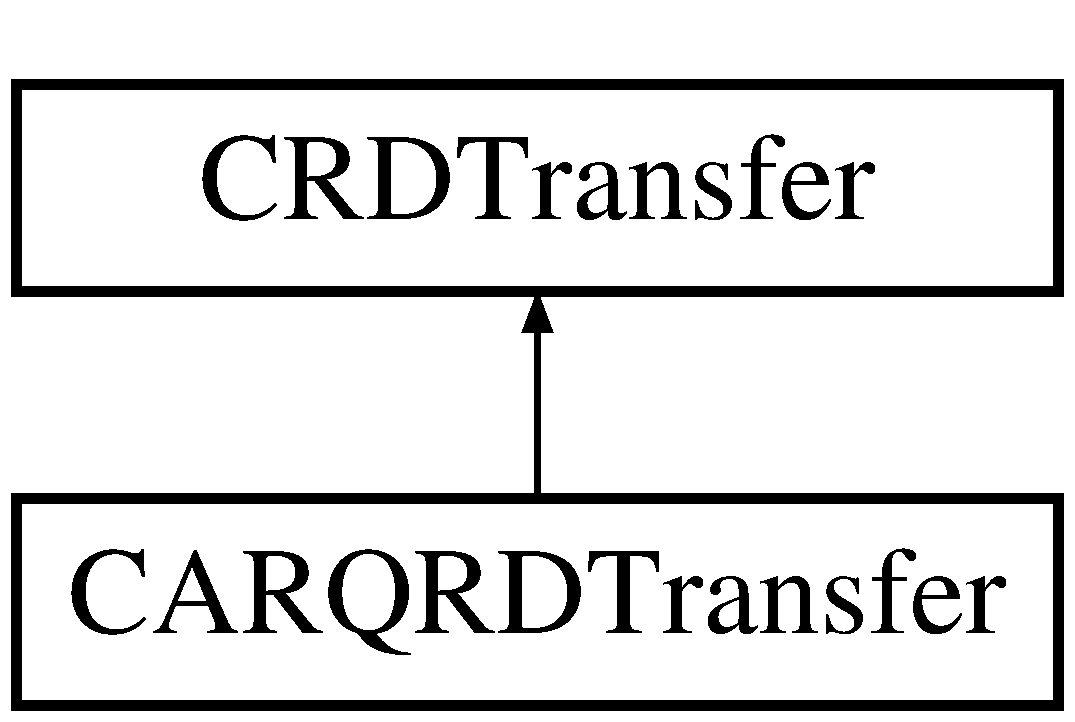
\includegraphics[height=2.000000cm]{class_c_a_r_q_r_d_transfer}
\end{center}
\end{figure}
\subsection*{额外继承的成员函数}


该类的文档由以下文件生成\+:\begin{DoxyCompactItemize}
\item 
G\+:/华中科技大学/计卓1401/大三下/计算机网络/\+Layer\+Interface/\+T\+C\+P\+Layer/A\+R\+Q\+R\+D\+Transfer.\+h\item 
G\+:/华中科技大学/计卓1401/大三下/计算机网络/\+Layer\+Interface/\+T\+C\+P\+Layer/A\+R\+Q\+R\+D\+Transfer.\+cpp\end{DoxyCompactItemize}

\hypertarget{class_c_a_r_q_trans}{}\section{C\+A\+R\+Q\+Trans类 参考}
\label{class_c_a_r_q_trans}\index{C\+A\+R\+Q\+Trans@{C\+A\+R\+Q\+Trans}}
类 C\+A\+R\+Q\+Trans 继承关系图\+:\begin{figure}[H]
\begin{center}
\leavevmode
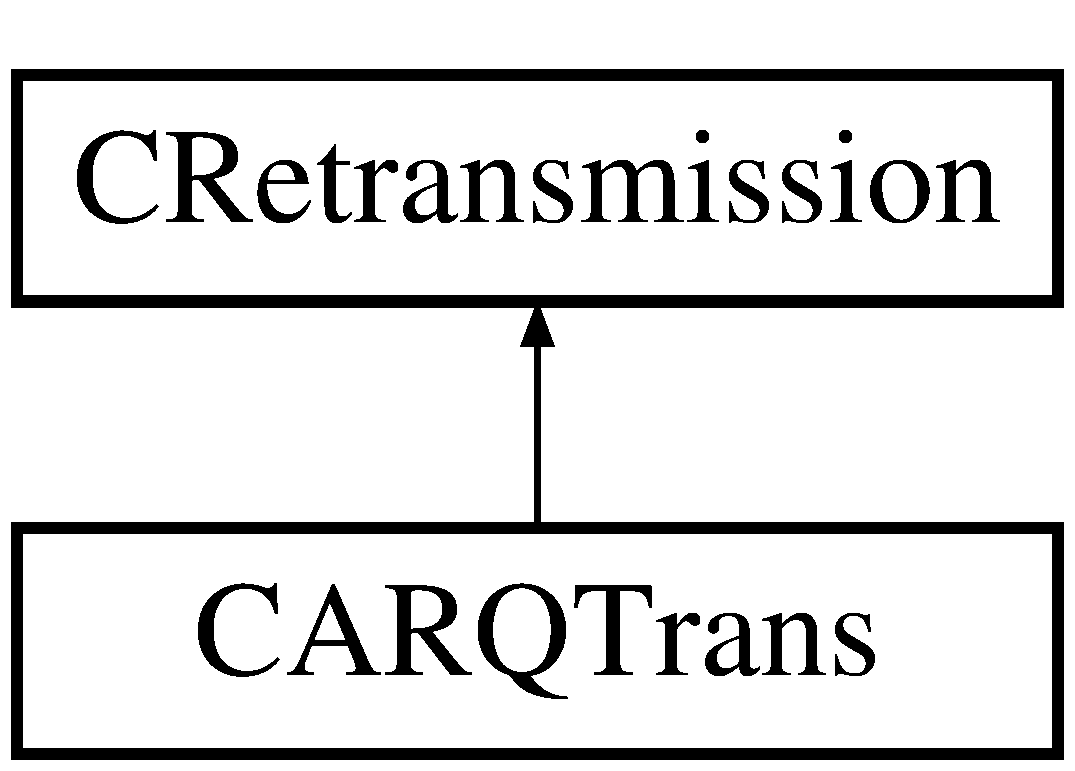
\includegraphics[height=2.000000cm]{class_c_a_r_q_trans}
\end{center}
\end{figure}
\subsection*{额外继承的成员函数}


该类的文档由以下文件生成\+:\begin{DoxyCompactItemize}
\item 
G\+:/华中科技大学/计卓1401/大三下/计算机网络/\+Layer\+Interface/\+Transport\+Layer/A\+R\+Q\+Trans.\+h\item 
G\+:/华中科技大学/计卓1401/大三下/计算机网络/\+Layer\+Interface/\+Transport\+Layer/A\+R\+Q\+Trans.\+cpp\end{DoxyCompactItemize}

\hypertarget{class_c_c_s_m_a___c_d}{}\section{C\+C\+S\+M\+A\+\_\+\+C\+D类 参考}
\label{class_c_c_s_m_a___c_d}\index{C\+C\+S\+M\+A\+\_\+\+CD@{C\+C\+S\+M\+A\+\_\+\+CD}}


{\ttfamily \#include $<$C\+S\+M\+A\+\_\+\+C\+D.\+h$>$}

\subsection*{Public 成员函数}
\begin{DoxyCompactItemize}
\item 
\hyperlink{class_c_c_s_m_a___c_d_a3558c5e07b179d60c2fc133bebee8e21}{C\+C\+S\+M\+A\+\_\+\+CD} ()
\item 
\hyperlink{class_c_c_s_m_a___c_d_a3b936d9a48b0c4d593f0bbff54761cbe}{$\sim$\+C\+C\+S\+M\+A\+\_\+\+CD} ()
\item 
void \hyperlink{class_c_c_s_m_a___c_d_a270a833b070a834dbf2c1f997ea85ee6}{monitor} ()
\item 
bool \hyperlink{class_c_c_s_m_a___c_d_a630a99c3ee32298d8c217a3fc2e2d65c}{send} ()
\item 
bool \hyperlink{class_c_c_s_m_a___c_d_a152628ee66959e6a2594250f51148be4}{detect} ()
\item 
void \hyperlink{class_c_c_s_m_a___c_d_a5ace5c0de3305086cd7ee31e6f601cd3}{handle} ()
\end{DoxyCompactItemize}


\subsection{详细描述}


在文件 C\+S\+M\+A\+\_\+\+C\+D.\+h 第 2 行定义.



\subsection{构造及析构函数说明}
\mbox{\Hypertarget{class_c_c_s_m_a___c_d_a3558c5e07b179d60c2fc133bebee8e21}\label{class_c_c_s_m_a___c_d_a3558c5e07b179d60c2fc133bebee8e21}} 
\index{C\+C\+S\+M\+A\+\_\+\+CD@{C\+C\+S\+M\+A\+\_\+\+CD}!C\+C\+S\+M\+A\+\_\+\+CD@{C\+C\+S\+M\+A\+\_\+\+CD}}
\index{C\+C\+S\+M\+A\+\_\+\+CD@{C\+C\+S\+M\+A\+\_\+\+CD}!C\+C\+S\+M\+A\+\_\+\+CD@{C\+C\+S\+M\+A\+\_\+\+CD}}
\subsubsection{\texorpdfstring{C\+C\+S\+M\+A\+\_\+\+C\+D()}{CCSMA\_CD()}}
{\footnotesize\ttfamily C\+C\+S\+M\+A\+\_\+\+C\+D\+::\+C\+C\+S\+M\+A\+\_\+\+CD (\begin{DoxyParamCaption}{ }\end{DoxyParamCaption})}



在文件 C\+S\+M\+A\+\_\+\+C\+D.\+cpp 第 5 行定义.

\mbox{\Hypertarget{class_c_c_s_m_a___c_d_a3b936d9a48b0c4d593f0bbff54761cbe}\label{class_c_c_s_m_a___c_d_a3b936d9a48b0c4d593f0bbff54761cbe}} 
\index{C\+C\+S\+M\+A\+\_\+\+CD@{C\+C\+S\+M\+A\+\_\+\+CD}!````~C\+C\+S\+M\+A\+\_\+\+CD@{$\sim$\+C\+C\+S\+M\+A\+\_\+\+CD}}
\index{````~C\+C\+S\+M\+A\+\_\+\+CD@{$\sim$\+C\+C\+S\+M\+A\+\_\+\+CD}!C\+C\+S\+M\+A\+\_\+\+CD@{C\+C\+S\+M\+A\+\_\+\+CD}}
\subsubsection{\texorpdfstring{$\sim$\+C\+C\+S\+M\+A\+\_\+\+C\+D()}{~CCSMA\_CD()}}
{\footnotesize\ttfamily C\+C\+S\+M\+A\+\_\+\+C\+D\+::$\sim$\+C\+C\+S\+M\+A\+\_\+\+CD (\begin{DoxyParamCaption}{ }\end{DoxyParamCaption})}



在文件 C\+S\+M\+A\+\_\+\+C\+D.\+cpp 第 10 行定义.



\subsection{成员函数说明}
\mbox{\Hypertarget{class_c_c_s_m_a___c_d_a152628ee66959e6a2594250f51148be4}\label{class_c_c_s_m_a___c_d_a152628ee66959e6a2594250f51148be4}} 
\index{C\+C\+S\+M\+A\+\_\+\+CD@{C\+C\+S\+M\+A\+\_\+\+CD}!detect@{detect}}
\index{detect@{detect}!C\+C\+S\+M\+A\+\_\+\+CD@{C\+C\+S\+M\+A\+\_\+\+CD}}
\subsubsection{\texorpdfstring{detect()}{detect()}}
{\footnotesize\ttfamily bool C\+C\+S\+M\+A\+\_\+\+C\+D\+::detect (\begin{DoxyParamCaption}{ }\end{DoxyParamCaption})}



在文件 C\+S\+M\+A\+\_\+\+C\+D.\+cpp 第 17 行定义.

\mbox{\Hypertarget{class_c_c_s_m_a___c_d_a5ace5c0de3305086cd7ee31e6f601cd3}\label{class_c_c_s_m_a___c_d_a5ace5c0de3305086cd7ee31e6f601cd3}} 
\index{C\+C\+S\+M\+A\+\_\+\+CD@{C\+C\+S\+M\+A\+\_\+\+CD}!handle@{handle}}
\index{handle@{handle}!C\+C\+S\+M\+A\+\_\+\+CD@{C\+C\+S\+M\+A\+\_\+\+CD}}
\subsubsection{\texorpdfstring{handle()}{handle()}}
{\footnotesize\ttfamily void C\+C\+S\+M\+A\+\_\+\+C\+D\+::handle (\begin{DoxyParamCaption}{ }\end{DoxyParamCaption})}



在文件 C\+S\+M\+A\+\_\+\+C\+D.\+cpp 第 18 行定义.

\mbox{\Hypertarget{class_c_c_s_m_a___c_d_a270a833b070a834dbf2c1f997ea85ee6}\label{class_c_c_s_m_a___c_d_a270a833b070a834dbf2c1f997ea85ee6}} 
\index{C\+C\+S\+M\+A\+\_\+\+CD@{C\+C\+S\+M\+A\+\_\+\+CD}!monitor@{monitor}}
\index{monitor@{monitor}!C\+C\+S\+M\+A\+\_\+\+CD@{C\+C\+S\+M\+A\+\_\+\+CD}}
\subsubsection{\texorpdfstring{monitor()}{monitor()}}
{\footnotesize\ttfamily void C\+C\+S\+M\+A\+\_\+\+C\+D\+::monitor (\begin{DoxyParamCaption}{ }\end{DoxyParamCaption})}



在文件 C\+S\+M\+A\+\_\+\+C\+D.\+cpp 第 15 行定义.

\mbox{\Hypertarget{class_c_c_s_m_a___c_d_a630a99c3ee32298d8c217a3fc2e2d65c}\label{class_c_c_s_m_a___c_d_a630a99c3ee32298d8c217a3fc2e2d65c}} 
\index{C\+C\+S\+M\+A\+\_\+\+CD@{C\+C\+S\+M\+A\+\_\+\+CD}!send@{send}}
\index{send@{send}!C\+C\+S\+M\+A\+\_\+\+CD@{C\+C\+S\+M\+A\+\_\+\+CD}}
\subsubsection{\texorpdfstring{send()}{send()}}
{\footnotesize\ttfamily bool C\+C\+S\+M\+A\+\_\+\+C\+D\+::send (\begin{DoxyParamCaption}{ }\end{DoxyParamCaption})}



在文件 C\+S\+M\+A\+\_\+\+C\+D.\+cpp 第 16 行定义.



该类的文档由以下文件生成\+:\begin{DoxyCompactItemize}
\item 
G\+:/华中科技大学/计卓1401/大三下/计算机网络/\+Layer\+Interface/\+Link\+Layer/\hyperlink{_c_s_m_a___c_d_8h}{C\+S\+M\+A\+\_\+\+C\+D.\+h}\item 
G\+:/华中科技大学/计卓1401/大三下/计算机网络/\+Layer\+Interface/\+Link\+Layer/\hyperlink{_c_s_m_a___c_d_8cpp}{C\+S\+M\+A\+\_\+\+C\+D.\+cpp}\end{DoxyCompactItemize}

\hypertarget{class_c_datagram_check}{}\section{C\+Datagram\+Check类 参考}
\label{class_c_datagram_check}\index{C\+Datagram\+Check@{C\+Datagram\+Check}}
\subsection*{Public 类型}
\begin{DoxyCompactItemize}
\item 
\mbox{\Hypertarget{class_c_datagram_check_a291cad3176f8806883c6285957431b64}\label{class_c_datagram_check_a291cad3176f8806883c6285957431b64}} 
enum {\bfseries C\+H\+C\+K\+\_\+\+M\+E\+T\+H\+OD} \{ {\bfseries C\+RC} = 1
 \}
\end{DoxyCompactItemize}
\subsection*{Public 成员函数}
\begin{DoxyCompactItemize}
\item 
\mbox{\Hypertarget{class_c_datagram_check_ac607f6742d36faec27f6462aefb6abaf}\label{class_c_datagram_check_ac607f6742d36faec27f6462aefb6abaf}} 
void {\bfseries set\+Para} (char $\ast$p\+Head, int ilength)
\item 
\mbox{\Hypertarget{class_c_datagram_check_a9f21ffeb4696f31eb8af68b09cf17686}\label{class_c_datagram_check_a9f21ffeb4696f31eb8af68b09cf17686}} 
int {\bfseries check} (int proto)
\end{DoxyCompactItemize}
\subsection*{Protected 成员函数}
\begin{DoxyCompactItemize}
\item 
\mbox{\Hypertarget{class_c_datagram_check_af7314fcfc87618386920fcb567f6f5d7}\label{class_c_datagram_check_af7314fcfc87618386920fcb567f6f5d7}} 
int {\bfseries C\+R\+Ccheck} ()
\end{DoxyCompactItemize}


该类的文档由以下文件生成\+:\begin{DoxyCompactItemize}
\item 
G\+:/华中科技大学/计卓1401/大三下/计算机网络/\+Layer\+Interface/\+Datagram\+Check/Datagram\+Check.\+h\item 
G\+:/华中科技大学/计卓1401/大三下/计算机网络/\+Layer\+Interface/\+Datagram\+Check/Datagram\+Check.\+cpp\end{DoxyCompactItemize}

\hypertarget{class_c_forward_tabel}{}\section{C\+Forward\+Tabel类 参考}
\label{class_c_forward_tabel}\index{C\+Forward\+Tabel@{C\+Forward\+Tabel}}
\subsection*{Public 成员函数}
\begin{DoxyCompactItemize}
\item 
\mbox{\Hypertarget{class_c_forward_tabel_afbc987ef5b55ab2fbc21721d47d623ad}\label{class_c_forward_tabel_afbc987ef5b55ab2fbc21721d47d623ad}} 
void {\bfseries modify} ()
\item 
\mbox{\Hypertarget{class_c_forward_tabel_a90efc1b05feb38559334c371a8e83019}\label{class_c_forward_tabel_a90efc1b05feb38559334c371a8e83019}} 
void {\bfseries query} ()
\end{DoxyCompactItemize}


该类的文档由以下文件生成\+:\begin{DoxyCompactItemize}
\item 
G\+:/华中科技大学/计卓1401/大三下/计算机网络/\+Layer\+Interface/\+I\+P\+Layer/Forward\+Tabel.\+h\item 
G\+:/华中科技大学/计卓1401/大三下/计算机网络/\+Layer\+Interface/\+I\+P\+Layer/Forward\+Tabel.\+cpp\end{DoxyCompactItemize}

\hypertarget{class_c_g_b_n_r_d_transfer}{}\section{C\+G\+B\+N\+R\+D\+Transfer类 参考}
\label{class_c_g_b_n_r_d_transfer}\index{C\+G\+B\+N\+R\+D\+Transfer@{C\+G\+B\+N\+R\+D\+Transfer}}


{\ttfamily \#include $<$G\+B\+N\+R\+D\+Transfer.\+h$>$}

类 C\+G\+B\+N\+R\+D\+Transfer 继承关系图\+:\begin{figure}[H]
\begin{center}
\leavevmode
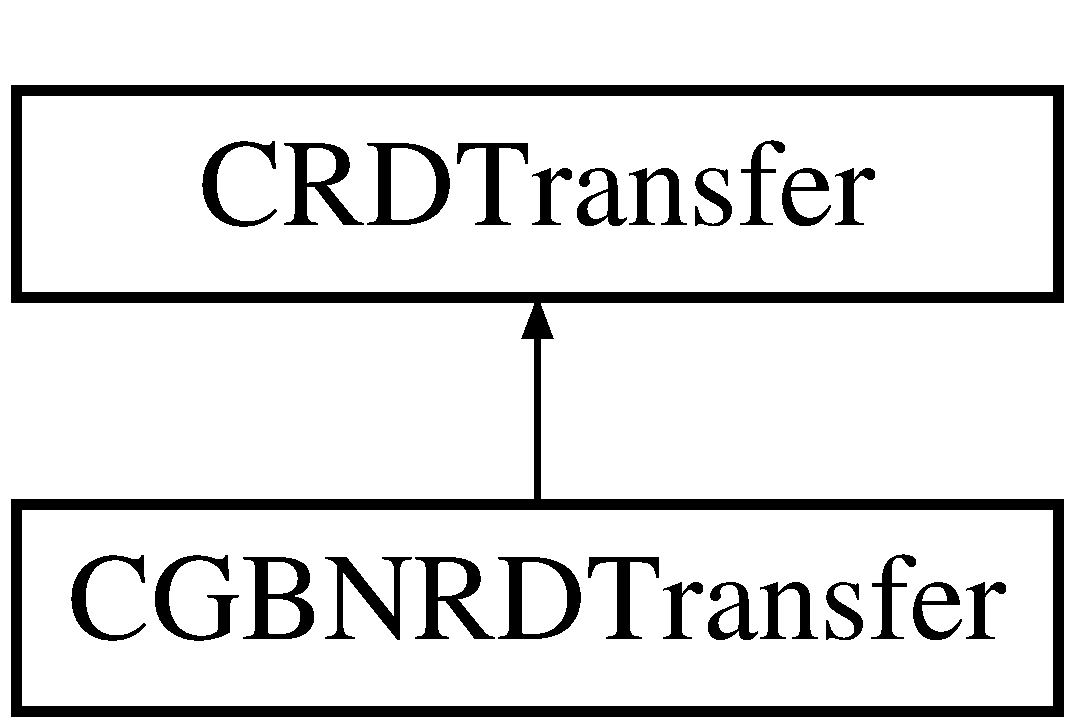
\includegraphics[height=2.000000cm]{class_c_g_b_n_r_d_transfer}
\end{center}
\end{figure}
\subsection*{Public 成员函数}
\begin{DoxyCompactItemize}
\item 
\hyperlink{class_c_g_b_n_r_d_transfer_a30a068efae62da055019080cf705067b}{C\+G\+B\+N\+R\+D\+Transfer} ()
\item 
\hyperlink{class_c_g_b_n_r_d_transfer_a4de477d40f503ddea1b4151933264fec}{$\sim$\+C\+G\+B\+N\+R\+D\+Transfer} ()
\end{DoxyCompactItemize}
\subsection*{额外继承的成员函数}


\subsection{详细描述}


在文件 G\+B\+N\+R\+D\+Transfer.\+h 第 3 行定义.



\subsection{构造及析构函数说明}
\mbox{\Hypertarget{class_c_g_b_n_r_d_transfer_a30a068efae62da055019080cf705067b}\label{class_c_g_b_n_r_d_transfer_a30a068efae62da055019080cf705067b}} 
\index{C\+G\+B\+N\+R\+D\+Transfer@{C\+G\+B\+N\+R\+D\+Transfer}!C\+G\+B\+N\+R\+D\+Transfer@{C\+G\+B\+N\+R\+D\+Transfer}}
\index{C\+G\+B\+N\+R\+D\+Transfer@{C\+G\+B\+N\+R\+D\+Transfer}!C\+G\+B\+N\+R\+D\+Transfer@{C\+G\+B\+N\+R\+D\+Transfer}}
\subsubsection{\texorpdfstring{C\+G\+B\+N\+R\+D\+Transfer()}{CGBNRDTransfer()}}
{\footnotesize\ttfamily C\+G\+B\+N\+R\+D\+Transfer\+::\+C\+G\+B\+N\+R\+D\+Transfer (\begin{DoxyParamCaption}{ }\end{DoxyParamCaption})}



在文件 G\+B\+N\+R\+D\+Transfer.\+cpp 第 5 行定义.

\mbox{\Hypertarget{class_c_g_b_n_r_d_transfer_a4de477d40f503ddea1b4151933264fec}\label{class_c_g_b_n_r_d_transfer_a4de477d40f503ddea1b4151933264fec}} 
\index{C\+G\+B\+N\+R\+D\+Transfer@{C\+G\+B\+N\+R\+D\+Transfer}!````~C\+G\+B\+N\+R\+D\+Transfer@{$\sim$\+C\+G\+B\+N\+R\+D\+Transfer}}
\index{````~C\+G\+B\+N\+R\+D\+Transfer@{$\sim$\+C\+G\+B\+N\+R\+D\+Transfer}!C\+G\+B\+N\+R\+D\+Transfer@{C\+G\+B\+N\+R\+D\+Transfer}}
\subsubsection{\texorpdfstring{$\sim$\+C\+G\+B\+N\+R\+D\+Transfer()}{~CGBNRDTransfer()}}
{\footnotesize\ttfamily C\+G\+B\+N\+R\+D\+Transfer\+::$\sim$\+C\+G\+B\+N\+R\+D\+Transfer (\begin{DoxyParamCaption}{ }\end{DoxyParamCaption})}



在文件 G\+B\+N\+R\+D\+Transfer.\+cpp 第 10 行定义.



该类的文档由以下文件生成\+:\begin{DoxyCompactItemize}
\item 
G\+:/华中科技大学/计卓1401/大三下/计算机网络/\+Layer\+Interface/\+T\+C\+P\+Layer/\hyperlink{_g_b_n_r_d_transfer_8h}{G\+B\+N\+R\+D\+Transfer.\+h}\item 
G\+:/华中科技大学/计卓1401/大三下/计算机网络/\+Layer\+Interface/\+T\+C\+P\+Layer/\hyperlink{_g_b_n_r_d_transfer_8cpp}{G\+B\+N\+R\+D\+Transfer.\+cpp}\end{DoxyCompactItemize}

\hypertarget{class_c_go_back_n_trans}{}\section{C\+Go\+Back\+N\+Trans类 参考}
\label{class_c_go_back_n_trans}\index{C\+Go\+Back\+N\+Trans@{C\+Go\+Back\+N\+Trans}}
类 C\+Go\+Back\+N\+Trans 继承关系图\+:\begin{figure}[H]
\begin{center}
\leavevmode
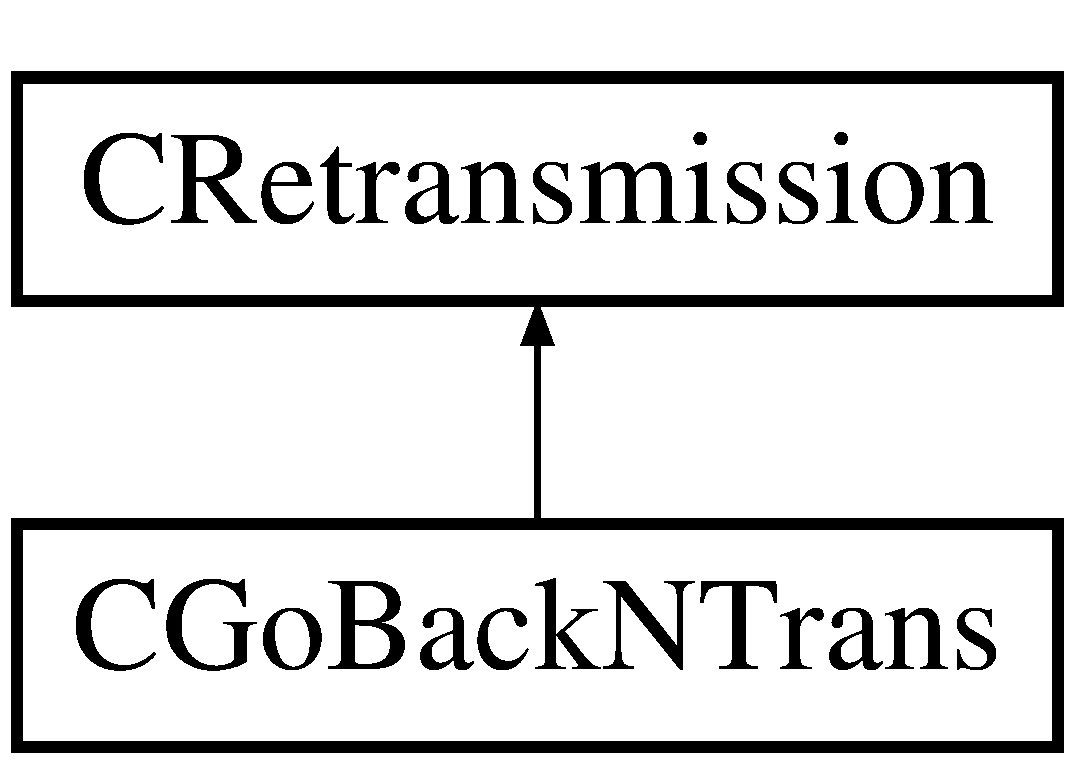
\includegraphics[height=2.000000cm]{class_c_go_back_n_trans}
\end{center}
\end{figure}
\subsection*{额外继承的成员函数}


该类的文档由以下文件生成\+:\begin{DoxyCompactItemize}
\item 
G\+:/华中科技大学/计卓1401/大三下/计算机网络/\+Layer\+Interface/\+Transport\+Layer/Go\+Back\+N\+Trans.\+h\item 
G\+:/华中科技大学/计卓1401/大三下/计算机网络/\+Layer\+Interface/\+Transport\+Layer/Go\+Back\+N\+Trans.\+cpp\end{DoxyCompactItemize}

\hypertarget{class_c_h_t_t_p}{}\section{C\+H\+T\+T\+P类 参考}
\label{class_c_h_t_t_p}\index{C\+H\+T\+TP@{C\+H\+T\+TP}}
\subsection*{Public 成员函数}
\begin{DoxyCompactItemize}
\item 
\mbox{\Hypertarget{class_c_h_t_t_p_a6c17fb2fe68967e23bd39012b1f70c68}\label{class_c_h_t_t_p_a6c17fb2fe68967e23bd39012b1f70c68}} 
{\bfseries C\+H\+T\+TP} (char $\ast$data, int length)
\item 
\mbox{\Hypertarget{class_c_h_t_t_p_a4866e1561e808229ff6244e866356741}\label{class_c_h_t_t_p_a4866e1561e808229ff6244e866356741}} 
char $\ast$ {\bfseries get\+Data} ()
\end{DoxyCompactItemize}
\subsection*{Public 属性}
\begin{DoxyCompactItemize}
\item 
\mbox{\Hypertarget{class_c_h_t_t_p_a0732dddaf54fa24a1554e566fcfa4eef}\label{class_c_h_t_t_p_a0732dddaf54fa24a1554e566fcfa4eef}} 
\hyperlink{class_c_u_d_p}{C\+U\+DP} $\ast$ {\bfseries tran\+Layer}
\item 
\mbox{\Hypertarget{class_c_h_t_t_p_a8cf28a01350c98fe3e4cbf4920da25c5}\label{class_c_h_t_t_p_a8cf28a01350c98fe3e4cbf4920da25c5}} 
\hyperlink{class_msg_list}{Msg\+List} {\bfseries send\+List}
\item 
\mbox{\Hypertarget{class_c_h_t_t_p_a86395cb3e64e45d31fda86b8e2ebf9dc}\label{class_c_h_t_t_p_a86395cb3e64e45d31fda86b8e2ebf9dc}} 
\hyperlink{class_msg_list}{Msg\+List} {\bfseries rcv\+List}
\end{DoxyCompactItemize}


该类的文档由以下文件生成\+:\begin{DoxyCompactItemize}
\item 
G\+:/华中科技大学/计卓1401/大三下/计算机网络/\+Layer\+Interface/\+H\+T\+T\+P/H\+T\+T\+P.\+h\item 
G\+:/华中科技大学/计卓1401/大三下/计算机网络/\+Layer\+Interface/\+H\+T\+T\+P/H\+T\+T\+P.\+cpp\end{DoxyCompactItemize}

\hypertarget{class_c_i_p_clip}{}\section{C\+I\+P\+Clip类 参考}
\label{class_c_i_p_clip}\index{C\+I\+P\+Clip@{C\+I\+P\+Clip}}


{\ttfamily \#include $<$I\+P\+Clip.\+h$>$}

\subsection*{Public 成员函数}
\begin{DoxyCompactItemize}
\item 
\hyperlink{class_c_i_p_clip_a19ef4a15f778c5d8cb8a064865422ee3}{C\+I\+P\+Clip} ()
\item 
\hyperlink{class_c_i_p_clip_a72b247b0bcf0dc6fcb41986f640bb4fa}{$\sim$\+C\+I\+P\+Clip} ()
\end{DoxyCompactItemize}


\subsection{详细描述}


在文件 I\+P\+Clip.\+h 第 2 行定义.



\subsection{构造及析构函数说明}
\mbox{\Hypertarget{class_c_i_p_clip_a19ef4a15f778c5d8cb8a064865422ee3}\label{class_c_i_p_clip_a19ef4a15f778c5d8cb8a064865422ee3}} 
\index{C\+I\+P\+Clip@{C\+I\+P\+Clip}!C\+I\+P\+Clip@{C\+I\+P\+Clip}}
\index{C\+I\+P\+Clip@{C\+I\+P\+Clip}!C\+I\+P\+Clip@{C\+I\+P\+Clip}}
\subsubsection{\texorpdfstring{C\+I\+P\+Clip()}{CIPClip()}}
{\footnotesize\ttfamily C\+I\+P\+Clip\+::\+C\+I\+P\+Clip (\begin{DoxyParamCaption}{ }\end{DoxyParamCaption})}



在文件 I\+P\+Clip.\+cpp 第 5 行定义.

\mbox{\Hypertarget{class_c_i_p_clip_a72b247b0bcf0dc6fcb41986f640bb4fa}\label{class_c_i_p_clip_a72b247b0bcf0dc6fcb41986f640bb4fa}} 
\index{C\+I\+P\+Clip@{C\+I\+P\+Clip}!````~C\+I\+P\+Clip@{$\sim$\+C\+I\+P\+Clip}}
\index{````~C\+I\+P\+Clip@{$\sim$\+C\+I\+P\+Clip}!C\+I\+P\+Clip@{C\+I\+P\+Clip}}
\subsubsection{\texorpdfstring{$\sim$\+C\+I\+P\+Clip()}{~CIPClip()}}
{\footnotesize\ttfamily C\+I\+P\+Clip\+::$\sim$\+C\+I\+P\+Clip (\begin{DoxyParamCaption}{ }\end{DoxyParamCaption})}



在文件 I\+P\+Clip.\+cpp 第 10 行定义.



该类的文档由以下文件生成\+:\begin{DoxyCompactItemize}
\item 
G\+:/华中科技大学/计卓1401/大三下/计算机网络/\+Layer\+Interface/\+I\+P\+Layer/\hyperlink{_i_p_clip_8h}{I\+P\+Clip.\+h}\item 
G\+:/华中科技大学/计卓1401/大三下/计算机网络/\+Layer\+Interface/\+I\+P\+Layer/\hyperlink{_i_p_clip_8cpp}{I\+P\+Clip.\+cpp}\end{DoxyCompactItemize}

\hypertarget{class_c_i_p_layer}{}\section{C\+I\+P\+Layer类 参考}
\label{class_c_i_p_layer}\index{C\+I\+P\+Layer@{C\+I\+P\+Layer}}


{\ttfamily \#include $<$I\+P\+Layer.\+h$>$}

类 C\+I\+P\+Layer 继承关系图\+:\begin{figure}[H]
\begin{center}
\leavevmode
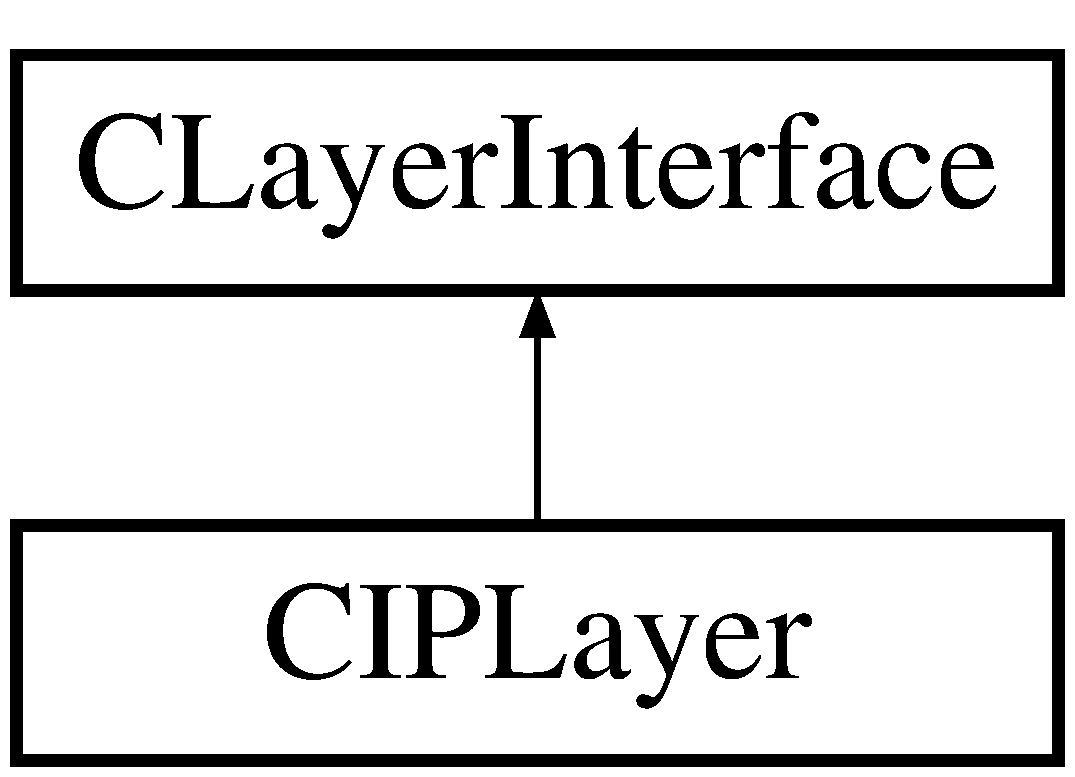
\includegraphics[height=2.000000cm]{class_c_i_p_layer}
\end{center}
\end{figure}
\subsection*{Public 成员函数}
\begin{DoxyCompactItemize}
\item 
\hyperlink{class_c_i_p_layer_a29f18d33abf037633c2dce2ed727ca5e}{C\+I\+P\+Layer} (\hyperlink{class_msg_list}{Msg\+List} \&send\+Buf, \hyperlink{class_msg_list}{Msg\+List} \&rcv\+Buf)
\item 
\hyperlink{class_c_i_p_layer_a064dc4bd7137c3c1a509ff3b9f23765a}{$\sim$\+C\+I\+P\+Layer} ()
\item 
void \hyperlink{class_c_i_p_layer_afe758e9d359f9318a026ac89672b4b21}{routing} ()
\item 
void \hyperlink{class_c_i_p_layer_a85c7f675704b8605eb16e881abdcca1d}{fragment} ()
\item 
void \hyperlink{class_c_i_p_layer_a68cfe267fa5138e11051d746540ae714}{reassemble} ()
\end{DoxyCompactItemize}
\subsection*{Protected 成员函数}
\begin{DoxyCompactItemize}
\item 
void \hyperlink{class_c_i_p_layer_a4a73e335cc0801fe2a7f0de6ab955411}{add\+Head} ()
\end{DoxyCompactItemize}
\subsection*{额外继承的成员函数}


\subsection{详细描述}


在文件 I\+P\+Layer.\+h 第 13 行定义.



\subsection{构造及析构函数说明}
\mbox{\Hypertarget{class_c_i_p_layer_a29f18d33abf037633c2dce2ed727ca5e}\label{class_c_i_p_layer_a29f18d33abf037633c2dce2ed727ca5e}} 
\index{C\+I\+P\+Layer@{C\+I\+P\+Layer}!C\+I\+P\+Layer@{C\+I\+P\+Layer}}
\index{C\+I\+P\+Layer@{C\+I\+P\+Layer}!C\+I\+P\+Layer@{C\+I\+P\+Layer}}
\subsubsection{\texorpdfstring{C\+I\+P\+Layer()}{CIPLayer()}}
{\footnotesize\ttfamily C\+I\+P\+Layer\+::\+C\+I\+P\+Layer (\begin{DoxyParamCaption}\item[{\hyperlink{class_msg_list}{Msg\+List} \&}]{send\+Buf,  }\item[{\hyperlink{class_msg_list}{Msg\+List} \&}]{rcv\+Buf }\end{DoxyParamCaption})}



在文件 I\+P\+Layer.\+cpp 第 10 行定义.

\mbox{\Hypertarget{class_c_i_p_layer_a064dc4bd7137c3c1a509ff3b9f23765a}\label{class_c_i_p_layer_a064dc4bd7137c3c1a509ff3b9f23765a}} 
\index{C\+I\+P\+Layer@{C\+I\+P\+Layer}!````~C\+I\+P\+Layer@{$\sim$\+C\+I\+P\+Layer}}
\index{````~C\+I\+P\+Layer@{$\sim$\+C\+I\+P\+Layer}!C\+I\+P\+Layer@{C\+I\+P\+Layer}}
\subsubsection{\texorpdfstring{$\sim$\+C\+I\+P\+Layer()}{~CIPLayer()}}
{\footnotesize\ttfamily C\+I\+P\+Layer\+::$\sim$\+C\+I\+P\+Layer (\begin{DoxyParamCaption}{ }\end{DoxyParamCaption})}



在文件 I\+P\+Layer.\+cpp 第 22 行定义.



\subsection{成员函数说明}
\mbox{\Hypertarget{class_c_i_p_layer_a4a73e335cc0801fe2a7f0de6ab955411}\label{class_c_i_p_layer_a4a73e335cc0801fe2a7f0de6ab955411}} 
\index{C\+I\+P\+Layer@{C\+I\+P\+Layer}!add\+Head@{add\+Head}}
\index{add\+Head@{add\+Head}!C\+I\+P\+Layer@{C\+I\+P\+Layer}}
\subsubsection{\texorpdfstring{add\+Head()}{addHead()}}
{\footnotesize\ttfamily void C\+I\+P\+Layer\+::add\+Head (\begin{DoxyParamCaption}{ }\end{DoxyParamCaption})\hspace{0.3cm}{\ttfamily [protected]}, {\ttfamily [virtual]}}



重载 \hyperlink{class_c_layer_interface_ac38c51660960657ac42e37a19ea062b4}{C\+Layer\+Interface} .



在文件 I\+P\+Layer.\+cpp 第 27 行定义.

\mbox{\Hypertarget{class_c_i_p_layer_a85c7f675704b8605eb16e881abdcca1d}\label{class_c_i_p_layer_a85c7f675704b8605eb16e881abdcca1d}} 
\index{C\+I\+P\+Layer@{C\+I\+P\+Layer}!fragment@{fragment}}
\index{fragment@{fragment}!C\+I\+P\+Layer@{C\+I\+P\+Layer}}
\subsubsection{\texorpdfstring{fragment()}{fragment()}}
{\footnotesize\ttfamily void C\+I\+P\+Layer\+::fragment (\begin{DoxyParamCaption}{ }\end{DoxyParamCaption})}

\mbox{\Hypertarget{class_c_i_p_layer_a68cfe267fa5138e11051d746540ae714}\label{class_c_i_p_layer_a68cfe267fa5138e11051d746540ae714}} 
\index{C\+I\+P\+Layer@{C\+I\+P\+Layer}!reassemble@{reassemble}}
\index{reassemble@{reassemble}!C\+I\+P\+Layer@{C\+I\+P\+Layer}}
\subsubsection{\texorpdfstring{reassemble()}{reassemble()}}
{\footnotesize\ttfamily void C\+I\+P\+Layer\+::reassemble (\begin{DoxyParamCaption}{ }\end{DoxyParamCaption})}

\mbox{\Hypertarget{class_c_i_p_layer_afe758e9d359f9318a026ac89672b4b21}\label{class_c_i_p_layer_afe758e9d359f9318a026ac89672b4b21}} 
\index{C\+I\+P\+Layer@{C\+I\+P\+Layer}!routing@{routing}}
\index{routing@{routing}!C\+I\+P\+Layer@{C\+I\+P\+Layer}}
\subsubsection{\texorpdfstring{routing()}{routing()}}
{\footnotesize\ttfamily void C\+I\+P\+Layer\+::routing (\begin{DoxyParamCaption}{ }\end{DoxyParamCaption})}



该类的文档由以下文件生成\+:\begin{DoxyCompactItemize}
\item 
G\+:/华中科技大学/计卓1401/大三下/计算机网络/\+Layer\+Interface/\+I\+P\+Layer/\hyperlink{_i_p_layer_8h}{I\+P\+Layer.\+h}\item 
G\+:/华中科技大学/计卓1401/大三下/计算机网络/\+Layer\+Interface/\+I\+P\+Layer/\hyperlink{_i_p_layer_8cpp}{I\+P\+Layer.\+cpp}\end{DoxyCompactItemize}

\hypertarget{class_c_layer_interface}{}\section{C\+Layer\+Interface类 参考}
\label{class_c_layer_interface}\index{C\+Layer\+Interface@{C\+Layer\+Interface}}


{\ttfamily \#include $<$Layer\+Interface.\+h$>$}

类 C\+Layer\+Interface 继承关系图\+:\begin{figure}[H]
\begin{center}
\leavevmode
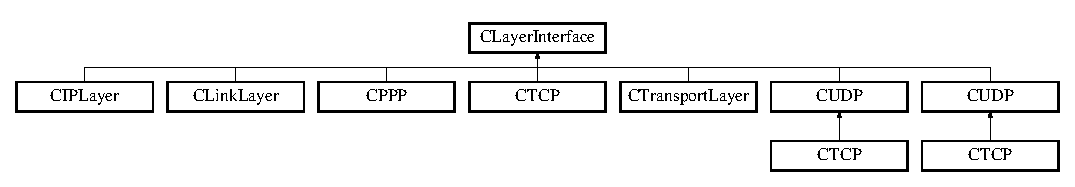
\includegraphics[height=2.068965cm]{class_c_layer_interface}
\end{center}
\end{figure}
\subsection*{Public 成员函数}
\begin{DoxyCompactItemize}
\item 
\hyperlink{class_c_layer_interface_a3001e0f4073b4499e4a1146e90de4100}{C\+Layer\+Interface} ()
\item 
\hyperlink{class_c_layer_interface_a505d26b4942bb87ece39152a71bcfb62}{C\+Layer\+Interface} (\hyperlink{class_msg_list}{Msg\+List} \&td, \hyperlink{class_msg_list}{Msg\+List} \&dt)
\item 
virtual \hyperlink{class_c_layer_interface_a75f554caabcadd933724685b9a7121a7}{$\sim$\+C\+Layer\+Interface} ()
\item 
bool \hyperlink{class_c_layer_interface_a82cdd178439031dd581a8f7208f2a134}{init} ()
\item 
void \hyperlink{class_c_layer_interface_a72740530fff12b29c8d1fb23aed88f2c}{run} ()
\item 
void \hyperlink{class_c_layer_interface_aa77c283e1d595a23513ff21cbf72ab97}{stop\+Run} ()
\item 
void \hyperlink{class_c_layer_interface_ad2d30dcc6415c22dd01f87114753d996}{layer\+Control} ()
\item 
virtual bool \hyperlink{class_c_layer_interface_a4979d7b5740c06be048e4b0f1195c8fc}{is\+Buffer\+Ready} (int lable)
\item 
virtual \hyperlink{class_datagram}{Datagram} \hyperlink{class_c_layer_interface_a804d604d3e0032e676d02fd5d369607e}{get\+Data} (int lable)
\item 
virtual bool \hyperlink{class_c_layer_interface_ae5115cf6ee0e76247dac067cc797a06b}{send\+Data} (\hyperlink{class_datagram}{Datagram} data)
\item 
virtual bool \hyperlink{class_c_layer_interface_a72415f0966b67359e0ee885d98827c3f}{recv\+Data} (\hyperlink{class_datagram}{Datagram} data)
\item 
void \hyperlink{class_c_layer_interface_a006961acbffa93cc0936010432b8e612}{set\+Head\+Tail\+Len} (int i\+Msg\+Head\+Len, int i\+Msg\+Tail\+Len)
\end{DoxyCompactItemize}
\subsection*{静态 Public 成员函数}
\begin{DoxyCompactItemize}
\item 
static D\+W\+O\+RD W\+I\+N\+A\+PI \hyperlink{class_c_layer_interface_a59d79b4c294ca20c2a761a4f1f737e24}{layer\+Thread} (L\+P\+V\+O\+ID lp\+Param)
\end{DoxyCompactItemize}
\subsection*{Protected 类型}
\begin{DoxyCompactItemize}
\item 
enum \{ \hyperlink{class_c_layer_interface_a033fd0915604b00e58a68115d414a50aa7eeac76b4b92f888cb8ac9bf1bb05eac}{S\+E\+R\+V\+ER} = 0, 
\hyperlink{class_c_layer_interface_a033fd0915604b00e58a68115d414a50aaca016d45c2bb91af5ffd4a1be97f1cd3}{C\+L\+I\+E\+NT}
 \}
\item 
enum \hyperlink{class_c_layer_interface_abcab6cee3a2b9a396b287124f4204756}{m\+\_\+\+Serv\+Proto\+Type} \{ \hyperlink{class_c_layer_interface_abcab6cee3a2b9a396b287124f4204756afcf9bb4eb22b22ecf8d2192c50e06026}{T\+CP}, 
\hyperlink{class_c_layer_interface_abcab6cee3a2b9a396b287124f4204756ac26954c1ead3d7a4cb6df8d1db2377e1}{U\+DP}, 
\hyperlink{class_c_layer_interface_abcab6cee3a2b9a396b287124f4204756a4f5637cbd0e6bd8f4f5d0198da841c15}{IP}
 \}
\end{DoxyCompactItemize}
\subsection*{Protected 成员函数}
\begin{DoxyCompactItemize}
\item 
virtual void \hyperlink{class_c_layer_interface_a4bde2a0310c9071cbe7020cc38c97674}{package} (\hyperlink{class_datagram}{Datagram} datagram)
\item 
virtual void \hyperlink{class_c_layer_interface_a94cb2e090328df13a252a2ea40db94d8}{unpack} ()
\item 
virtual void \hyperlink{class_c_layer_interface_ac38c51660960657ac42e37a19ea062b4}{add\+Head} ()
\item 
virtual void \hyperlink{class_c_layer_interface_a433a6f3322355291bbfc2b97343d493f}{add\+Tail} ()
\item 
void \hyperlink{class_c_layer_interface_ac98e8ced890a29b4b76e16cfa3defddb}{rmv\+Head\+Buf} ()
\item 
virtual void \hyperlink{class_c_layer_interface_a02a144b97e69df2dc47149e5314cba2d}{send\+Transfer} ()
\item 
virtual void \hyperlink{class_c_layer_interface_aca72cd6ae77b4e4b4c1d058377583110}{recv\+Transfer} ()
\end{DoxyCompactItemize}
\subsection*{Protected 属性}
\begin{DoxyCompactItemize}
\item 
bool \hyperlink{class_c_layer_interface_a21292dad42f0048a08a19eeeba0d68cc}{b\+Stop}
\item 
\hyperlink{class_c_layer_interface}{C\+Layer\+Interface} $\ast$ \hyperlink{class_c_layer_interface_a075d83e440db42925a85d17f9e3e9a0b}{p\+Server\+Layer}
\item 
bool \hyperlink{class_c_layer_interface_ab5e0e1580b714b045664a8051373b8f2}{b\+Has\+Server\+Layer}
\item 
\hyperlink{class_datagram}{Datagram} $\ast$ \hyperlink{class_c_layer_interface_a6c3c04e1123c94ff609dafbd2429dfee}{m\+\_\+p\+Datagram}
\item 
int \hyperlink{class_c_layer_interface_a7057ebc9a57429562f4642b5e8586a52}{m\+\_\+n\+Msg\+Head\+Len}
\item 
int \hyperlink{class_c_layer_interface_a6c9d5fd635c29705c2cb9bea7c5a68f5}{m\+\_\+n\+Msg\+Tail\+Len}
\item 
\hyperlink{class_msg_list}{Msg\+List} \hyperlink{class_c_layer_interface_ab85631c424f3a77311ca4532db18d8a6}{my\+Send\+Buf}
\item 
\hyperlink{class_msg_list}{Msg\+List} \hyperlink{class_c_layer_interface_a6b35060c9d58ff2a0f394e1c54301ae8}{my\+Recv\+Buf}
\item 
\hyperlink{class_msg_list}{Msg\+List} \& \hyperlink{class_c_layer_interface_a17da1d50a68115d810b8079f1c6e22d7}{m\+\_\+p\+Client\+Send\+Buf}
\item 
\hyperlink{class_msg_list}{Msg\+List} \& \hyperlink{class_c_layer_interface_af9509b975b79a1c15a5a5523c03eeaaa}{m\+\_\+p\+Client\+Rcv\+Buf}
\item 
\hyperlink{_layer_interface_2_mail_slot_8h_aa8c0374618b33785ccb02f74bcfebc46}{H\+A\+N\+D\+LE} \hyperlink{class_c_layer_interface_a91818359711b0f61e18347707a13ba31}{h\+Thread}
\end{DoxyCompactItemize}


\subsection{详细描述}


在文件 Layer\+Interface.\+h 第 28 行定义.



\subsection{成员枚举类型说明}
\mbox{\Hypertarget{class_c_layer_interface_a033fd0915604b00e58a68115d414a50a}\label{class_c_layer_interface_a033fd0915604b00e58a68115d414a50a}} 
\subsubsection{\texorpdfstring{anonymous enum}{anonymous enum}}
{\footnotesize\ttfamily anonymous enum\hspace{0.3cm}{\ttfamily [protected]}}

\begin{DoxyEnumFields}{枚举值}
\raisebox{\heightof{T}}[0pt][0pt]{\index{S\+E\+R\+V\+ER@{S\+E\+R\+V\+ER}!C\+Layer\+Interface@{C\+Layer\+Interface}}\index{C\+Layer\+Interface@{C\+Layer\+Interface}!S\+E\+R\+V\+ER@{S\+E\+R\+V\+ER}}}\mbox{\Hypertarget{class_c_layer_interface_a033fd0915604b00e58a68115d414a50aa7eeac76b4b92f888cb8ac9bf1bb05eac}\label{class_c_layer_interface_a033fd0915604b00e58a68115d414a50aa7eeac76b4b92f888cb8ac9bf1bb05eac}} 
S\+E\+R\+V\+ER&\\
\hline

\raisebox{\heightof{T}}[0pt][0pt]{\index{C\+L\+I\+E\+NT@{C\+L\+I\+E\+NT}!C\+Layer\+Interface@{C\+Layer\+Interface}}\index{C\+Layer\+Interface@{C\+Layer\+Interface}!C\+L\+I\+E\+NT@{C\+L\+I\+E\+NT}}}\mbox{\Hypertarget{class_c_layer_interface_a033fd0915604b00e58a68115d414a50aaca016d45c2bb91af5ffd4a1be97f1cd3}\label{class_c_layer_interface_a033fd0915604b00e58a68115d414a50aaca016d45c2bb91af5ffd4a1be97f1cd3}} 
C\+L\+I\+E\+NT&\\
\hline

\end{DoxyEnumFields}


在文件 Layer\+Interface.\+h 第 56 行定义.

\mbox{\Hypertarget{class_c_layer_interface_abcab6cee3a2b9a396b287124f4204756}\label{class_c_layer_interface_abcab6cee3a2b9a396b287124f4204756}} 
\index{C\+Layer\+Interface@{C\+Layer\+Interface}!m\+\_\+\+Serv\+Proto\+Type@{m\+\_\+\+Serv\+Proto\+Type}}
\index{m\+\_\+\+Serv\+Proto\+Type@{m\+\_\+\+Serv\+Proto\+Type}!C\+Layer\+Interface@{C\+Layer\+Interface}}
\subsubsection{\texorpdfstring{m\+\_\+\+Serv\+Proto\+Type}{m\_ServProtoType}}
{\footnotesize\ttfamily enum \hyperlink{class_c_layer_interface_abcab6cee3a2b9a396b287124f4204756}{C\+Layer\+Interface\+::m\+\_\+\+Serv\+Proto\+Type}\hspace{0.3cm}{\ttfamily [protected]}}

\begin{DoxyEnumFields}{枚举值}
\raisebox{\heightof{T}}[0pt][0pt]{\index{T\+CP@{T\+CP}!C\+Layer\+Interface@{C\+Layer\+Interface}}\index{C\+Layer\+Interface@{C\+Layer\+Interface}!T\+CP@{T\+CP}}}\mbox{\Hypertarget{class_c_layer_interface_abcab6cee3a2b9a396b287124f4204756afcf9bb4eb22b22ecf8d2192c50e06026}\label{class_c_layer_interface_abcab6cee3a2b9a396b287124f4204756afcf9bb4eb22b22ecf8d2192c50e06026}} 
T\+CP&\\
\hline

\raisebox{\heightof{T}}[0pt][0pt]{\index{U\+DP@{U\+DP}!C\+Layer\+Interface@{C\+Layer\+Interface}}\index{C\+Layer\+Interface@{C\+Layer\+Interface}!U\+DP@{U\+DP}}}\mbox{\Hypertarget{class_c_layer_interface_abcab6cee3a2b9a396b287124f4204756ac26954c1ead3d7a4cb6df8d1db2377e1}\label{class_c_layer_interface_abcab6cee3a2b9a396b287124f4204756ac26954c1ead3d7a4cb6df8d1db2377e1}} 
U\+DP&\\
\hline

\raisebox{\heightof{T}}[0pt][0pt]{\index{IP@{IP}!C\+Layer\+Interface@{C\+Layer\+Interface}}\index{C\+Layer\+Interface@{C\+Layer\+Interface}!IP@{IP}}}\mbox{\Hypertarget{class_c_layer_interface_abcab6cee3a2b9a396b287124f4204756a4f5637cbd0e6bd8f4f5d0198da841c15}\label{class_c_layer_interface_abcab6cee3a2b9a396b287124f4204756a4f5637cbd0e6bd8f4f5d0198da841c15}} 
IP&\\
\hline

\end{DoxyEnumFields}


在文件 Layer\+Interface.\+h 第 73 行定义.



\subsection{构造及析构函数说明}
\mbox{\Hypertarget{class_c_layer_interface_a3001e0f4073b4499e4a1146e90de4100}\label{class_c_layer_interface_a3001e0f4073b4499e4a1146e90de4100}} 
\index{C\+Layer\+Interface@{C\+Layer\+Interface}!C\+Layer\+Interface@{C\+Layer\+Interface}}
\index{C\+Layer\+Interface@{C\+Layer\+Interface}!C\+Layer\+Interface@{C\+Layer\+Interface}}
\subsubsection{\texorpdfstring{C\+Layer\+Interface()}{CLayerInterface()}\hspace{0.1cm}{\footnotesize\ttfamily [1/2]}}
{\footnotesize\ttfamily C\+Layer\+Interface\+::\+C\+Layer\+Interface (\begin{DoxyParamCaption}{ }\end{DoxyParamCaption})}



在文件 Layer\+Interface.\+cpp 第 8 行定义.

\mbox{\Hypertarget{class_c_layer_interface_a505d26b4942bb87ece39152a71bcfb62}\label{class_c_layer_interface_a505d26b4942bb87ece39152a71bcfb62}} 
\index{C\+Layer\+Interface@{C\+Layer\+Interface}!C\+Layer\+Interface@{C\+Layer\+Interface}}
\index{C\+Layer\+Interface@{C\+Layer\+Interface}!C\+Layer\+Interface@{C\+Layer\+Interface}}
\subsubsection{\texorpdfstring{C\+Layer\+Interface()}{CLayerInterface()}\hspace{0.1cm}{\footnotesize\ttfamily [2/2]}}
{\footnotesize\ttfamily C\+Layer\+Interface\+::\+C\+Layer\+Interface (\begin{DoxyParamCaption}\item[{\hyperlink{class_msg_list}{Msg\+List} \&}]{td,  }\item[{\hyperlink{class_msg_list}{Msg\+List} \&}]{dt }\end{DoxyParamCaption})}

重载构造函数 

在文件 Layer\+Interface.\+cpp 第 12 行定义.

\mbox{\Hypertarget{class_c_layer_interface_a75f554caabcadd933724685b9a7121a7}\label{class_c_layer_interface_a75f554caabcadd933724685b9a7121a7}} 
\index{C\+Layer\+Interface@{C\+Layer\+Interface}!````~C\+Layer\+Interface@{$\sim$\+C\+Layer\+Interface}}
\index{````~C\+Layer\+Interface@{$\sim$\+C\+Layer\+Interface}!C\+Layer\+Interface@{C\+Layer\+Interface}}
\subsubsection{\texorpdfstring{$\sim$\+C\+Layer\+Interface()}{~CLayerInterface()}}
{\footnotesize\ttfamily C\+Layer\+Interface\+::$\sim$\+C\+Layer\+Interface (\begin{DoxyParamCaption}{ }\end{DoxyParamCaption})\hspace{0.3cm}{\ttfamily [virtual]}}



在文件 Layer\+Interface.\+cpp 第 37 行定义.



\subsection{成员函数说明}
\mbox{\Hypertarget{class_c_layer_interface_ac38c51660960657ac42e37a19ea062b4}\label{class_c_layer_interface_ac38c51660960657ac42e37a19ea062b4}} 
\index{C\+Layer\+Interface@{C\+Layer\+Interface}!add\+Head@{add\+Head}}
\index{add\+Head@{add\+Head}!C\+Layer\+Interface@{C\+Layer\+Interface}}
\subsubsection{\texorpdfstring{add\+Head()}{addHead()}}
{\footnotesize\ttfamily virtual void C\+Layer\+Interface\+::add\+Head (\begin{DoxyParamCaption}{ }\end{DoxyParamCaption})\hspace{0.3cm}{\ttfamily [inline]}, {\ttfamily [protected]}, {\ttfamily [virtual]}}



被 \hyperlink{class_c_i_p_layer_a4a73e335cc0801fe2a7f0de6ab955411}{C\+I\+P\+Layer}, \hyperlink{class_c_t_c_p_a0c68800a3b6317cbe74aa2cb28ea3d9c}{C\+T\+CP}, \hyperlink{class_c_u_d_p_a445c3b7fe1b58e8b278115649ad25c3f}{C\+U\+DP}, \hyperlink{class_c_link_layer_a6ef143071b324acea3cd11ef86ba850f}{C\+Link\+Layer}, \hyperlink{class_c_u_d_p_a445c3b7fe1b58e8b278115649ad25c3f}{C\+U\+DP}, \hyperlink{class_c_p_p_p_aba6a014532e6d329cf1f8dfb591eff72}{C\+P\+PP} , 以及 \hyperlink{class_c_t_c_p_a0c68800a3b6317cbe74aa2cb28ea3d9c}{C\+T\+CP} 重载.



在文件 Layer\+Interface.\+h 第 48 行定义.

\mbox{\Hypertarget{class_c_layer_interface_a433a6f3322355291bbfc2b97343d493f}\label{class_c_layer_interface_a433a6f3322355291bbfc2b97343d493f}} 
\index{C\+Layer\+Interface@{C\+Layer\+Interface}!add\+Tail@{add\+Tail}}
\index{add\+Tail@{add\+Tail}!C\+Layer\+Interface@{C\+Layer\+Interface}}
\subsubsection{\texorpdfstring{add\+Tail()}{addTail()}}
{\footnotesize\ttfamily virtual void C\+Layer\+Interface\+::add\+Tail (\begin{DoxyParamCaption}{ }\end{DoxyParamCaption})\hspace{0.3cm}{\ttfamily [inline]}, {\ttfamily [protected]}, {\ttfamily [virtual]}}



被 \hyperlink{class_c_link_layer_a0962e4887e1893721031309a1e49a638}{C\+Link\+Layer} , 以及 \hyperlink{class_c_p_p_p_a2b345908338ada3b4d9e58d14270725a}{C\+P\+PP} 重载.



在文件 Layer\+Interface.\+h 第 49 行定义.

\mbox{\Hypertarget{class_c_layer_interface_a804d604d3e0032e676d02fd5d369607e}\label{class_c_layer_interface_a804d604d3e0032e676d02fd5d369607e}} 
\index{C\+Layer\+Interface@{C\+Layer\+Interface}!get\+Data@{get\+Data}}
\index{get\+Data@{get\+Data}!C\+Layer\+Interface@{C\+Layer\+Interface}}
\subsubsection{\texorpdfstring{get\+Data()}{getData()}}
{\footnotesize\ttfamily \hyperlink{class_datagram}{Datagram} C\+Layer\+Interface\+::get\+Data (\begin{DoxyParamCaption}\item[{int}]{lable }\end{DoxyParamCaption})\hspace{0.3cm}{\ttfamily [virtual]}}

get data from the buffer 

被 \hyperlink{class_c_transport_layer_a9396850eb026ff070c06bfc25dd4979c}{C\+Transport\+Layer} , 以及 \hyperlink{class_c_u_d_p_aa71e49c760769b55dc2251b244eb00ff}{C\+U\+DP} 重载.



在文件 Layer\+Interface.\+cpp 第 93 行定义.

\mbox{\Hypertarget{class_c_layer_interface_a82cdd178439031dd581a8f7208f2a134}\label{class_c_layer_interface_a82cdd178439031dd581a8f7208f2a134}} 
\index{C\+Layer\+Interface@{C\+Layer\+Interface}!init@{init}}
\index{init@{init}!C\+Layer\+Interface@{C\+Layer\+Interface}}
\subsubsection{\texorpdfstring{init()}{init()}}
{\footnotesize\ttfamily bool C\+Layer\+Interface\+::init (\begin{DoxyParamCaption}{ }\end{DoxyParamCaption})}



在文件 Layer\+Interface.\+cpp 第 21 行定义.

\mbox{\Hypertarget{class_c_layer_interface_a4979d7b5740c06be048e4b0f1195c8fc}\label{class_c_layer_interface_a4979d7b5740c06be048e4b0f1195c8fc}} 
\index{C\+Layer\+Interface@{C\+Layer\+Interface}!is\+Buffer\+Ready@{is\+Buffer\+Ready}}
\index{is\+Buffer\+Ready@{is\+Buffer\+Ready}!C\+Layer\+Interface@{C\+Layer\+Interface}}
\subsubsection{\texorpdfstring{is\+Buffer\+Ready()}{isBufferReady()}}
{\footnotesize\ttfamily bool C\+Layer\+Interface\+::is\+Buffer\+Ready (\begin{DoxyParamCaption}\item[{int}]{lable }\end{DoxyParamCaption})\hspace{0.3cm}{\ttfamily [virtual]}}

check if the buffer can be used 

被 \hyperlink{class_c_transport_layer_aace17995c3cff74c756ecdb2a2e8cf43}{C\+Transport\+Layer} , 以及 \hyperlink{class_c_u_d_p_af595428bc531576d9859a9e0b84d03d9}{C\+U\+DP} 重载.



在文件 Layer\+Interface.\+cpp 第 83 行定义.

\mbox{\Hypertarget{class_c_layer_interface_ad2d30dcc6415c22dd01f87114753d996}\label{class_c_layer_interface_ad2d30dcc6415c22dd01f87114753d996}} 
\index{C\+Layer\+Interface@{C\+Layer\+Interface}!layer\+Control@{layer\+Control}}
\index{layer\+Control@{layer\+Control}!C\+Layer\+Interface@{C\+Layer\+Interface}}
\subsubsection{\texorpdfstring{layer\+Control()}{layerControl()}}
{\footnotesize\ttfamily void C\+Layer\+Interface\+::layer\+Control (\begin{DoxyParamCaption}{ }\end{DoxyParamCaption})}

\mbox{\Hypertarget{class_c_layer_interface_a59d79b4c294ca20c2a761a4f1f737e24}\label{class_c_layer_interface_a59d79b4c294ca20c2a761a4f1f737e24}} 
\index{C\+Layer\+Interface@{C\+Layer\+Interface}!layer\+Thread@{layer\+Thread}}
\index{layer\+Thread@{layer\+Thread}!C\+Layer\+Interface@{C\+Layer\+Interface}}
\subsubsection{\texorpdfstring{layer\+Thread()}{layerThread()}}
{\footnotesize\ttfamily D\+W\+O\+RD W\+I\+N\+A\+PI C\+Layer\+Interface\+::layer\+Thread (\begin{DoxyParamCaption}\item[{L\+P\+V\+O\+ID}]{lp\+Param }\end{DoxyParamCaption})\hspace{0.3cm}{\ttfamily [static]}}



在文件 Layer\+Interface.\+cpp 第 60 行定义.

\mbox{\Hypertarget{class_c_layer_interface_a4bde2a0310c9071cbe7020cc38c97674}\label{class_c_layer_interface_a4bde2a0310c9071cbe7020cc38c97674}} 
\index{C\+Layer\+Interface@{C\+Layer\+Interface}!package@{package}}
\index{package@{package}!C\+Layer\+Interface@{C\+Layer\+Interface}}
\subsubsection{\texorpdfstring{package()}{package()}}
{\footnotesize\ttfamily void C\+Layer\+Interface\+::package (\begin{DoxyParamCaption}\item[{\hyperlink{class_datagram}{Datagram}}]{datagram }\end{DoxyParamCaption})\hspace{0.3cm}{\ttfamily [protected]}, {\ttfamily [virtual]}}



在文件 Layer\+Interface.\+cpp 第 121 行定义.

\mbox{\Hypertarget{class_c_layer_interface_a72415f0966b67359e0ee885d98827c3f}\label{class_c_layer_interface_a72415f0966b67359e0ee885d98827c3f}} 
\index{C\+Layer\+Interface@{C\+Layer\+Interface}!recv\+Data@{recv\+Data}}
\index{recv\+Data@{recv\+Data}!C\+Layer\+Interface@{C\+Layer\+Interface}}
\subsubsection{\texorpdfstring{recv\+Data()}{recvData()}}
{\footnotesize\ttfamily bool C\+Layer\+Interface\+::recv\+Data (\begin{DoxyParamCaption}\item[{\hyperlink{class_datagram}{Datagram}}]{data }\end{DoxyParamCaption})\hspace{0.3cm}{\ttfamily [virtual]}}



被 \hyperlink{class_c_t_c_p_aed8fdd632e22efee66dbbb95e951b5c2}{C\+T\+CP} 重载.



在文件 Layer\+Interface.\+cpp 第 114 行定义.

\mbox{\Hypertarget{class_c_layer_interface_aca72cd6ae77b4e4b4c1d058377583110}\label{class_c_layer_interface_aca72cd6ae77b4e4b4c1d058377583110}} 
\index{C\+Layer\+Interface@{C\+Layer\+Interface}!recv\+Transfer@{recv\+Transfer}}
\index{recv\+Transfer@{recv\+Transfer}!C\+Layer\+Interface@{C\+Layer\+Interface}}
\subsubsection{\texorpdfstring{recv\+Transfer()}{recvTransfer()}}
{\footnotesize\ttfamily void C\+Layer\+Interface\+::recv\+Transfer (\begin{DoxyParamCaption}{ }\end{DoxyParamCaption})\hspace{0.3cm}{\ttfamily [protected]}, {\ttfamily [virtual]}}



被 \hyperlink{class_c_transport_layer_ad30133ccd6047d127d5a9feec593877d}{C\+Transport\+Layer} 重载.



在文件 Layer\+Interface.\+cpp 第 138 行定义.

\mbox{\Hypertarget{class_c_layer_interface_ac98e8ced890a29b4b76e16cfa3defddb}\label{class_c_layer_interface_ac98e8ced890a29b4b76e16cfa3defddb}} 
\index{C\+Layer\+Interface@{C\+Layer\+Interface}!rmv\+Head\+Buf@{rmv\+Head\+Buf}}
\index{rmv\+Head\+Buf@{rmv\+Head\+Buf}!C\+Layer\+Interface@{C\+Layer\+Interface}}
\subsubsection{\texorpdfstring{rmv\+Head\+Buf()}{rmvHeadBuf()}}
{\footnotesize\ttfamily void C\+Layer\+Interface\+::rmv\+Head\+Buf (\begin{DoxyParamCaption}{ }\end{DoxyParamCaption})\hspace{0.3cm}{\ttfamily [protected]}}



在文件 Layer\+Interface.\+cpp 第 132 行定义.

\mbox{\Hypertarget{class_c_layer_interface_a72740530fff12b29c8d1fb23aed88f2c}\label{class_c_layer_interface_a72740530fff12b29c8d1fb23aed88f2c}} 
\index{C\+Layer\+Interface@{C\+Layer\+Interface}!run@{run}}
\index{run@{run}!C\+Layer\+Interface@{C\+Layer\+Interface}}
\subsubsection{\texorpdfstring{run()}{run()}}
{\footnotesize\ttfamily void C\+Layer\+Interface\+::run (\begin{DoxyParamCaption}{ }\end{DoxyParamCaption})}



在文件 Layer\+Interface.\+cpp 第 50 行定义.

\mbox{\Hypertarget{class_c_layer_interface_ae5115cf6ee0e76247dac067cc797a06b}\label{class_c_layer_interface_ae5115cf6ee0e76247dac067cc797a06b}} 
\index{C\+Layer\+Interface@{C\+Layer\+Interface}!send\+Data@{send\+Data}}
\index{send\+Data@{send\+Data}!C\+Layer\+Interface@{C\+Layer\+Interface}}
\subsubsection{\texorpdfstring{send\+Data()}{sendData()}}
{\footnotesize\ttfamily bool C\+Layer\+Interface\+::send\+Data (\begin{DoxyParamCaption}\item[{\hyperlink{class_datagram}{Datagram}}]{data }\end{DoxyParamCaption})\hspace{0.3cm}{\ttfamily [virtual]}}

insert the data into buffer 

被 \hyperlink{class_c_t_c_p_a4552b74145e832f32c1cb45a9fa2a5e9}{C\+T\+CP} , 以及 \hyperlink{class_c_u_d_p_a1f6e555ad4997b283e68ebfa7dc0d263}{C\+U\+DP} 重载.



在文件 Layer\+Interface.\+cpp 第 103 行定义.

\mbox{\Hypertarget{class_c_layer_interface_a02a144b97e69df2dc47149e5314cba2d}\label{class_c_layer_interface_a02a144b97e69df2dc47149e5314cba2d}} 
\index{C\+Layer\+Interface@{C\+Layer\+Interface}!send\+Transfer@{send\+Transfer}}
\index{send\+Transfer@{send\+Transfer}!C\+Layer\+Interface@{C\+Layer\+Interface}}
\subsubsection{\texorpdfstring{send\+Transfer()}{sendTransfer()}}
{\footnotesize\ttfamily void C\+Layer\+Interface\+::send\+Transfer (\begin{DoxyParamCaption}{ }\end{DoxyParamCaption})\hspace{0.3cm}{\ttfamily [protected]}, {\ttfamily [virtual]}}



被 \hyperlink{class_c_transport_layer_a5755c5d7f4158bb08303b98042b24ca1}{C\+Transport\+Layer}, \hyperlink{class_c_link_layer_ab6a4124af45069fefeddff784ea26e3f}{C\+Link\+Layer} , 以及 \hyperlink{class_c_p_p_p_a1d8be0d39e44ad6e6971329106e5900d}{C\+P\+PP} 重载.



在文件 Layer\+Interface.\+cpp 第 149 行定义.

\mbox{\Hypertarget{class_c_layer_interface_a006961acbffa93cc0936010432b8e612}\label{class_c_layer_interface_a006961acbffa93cc0936010432b8e612}} 
\index{C\+Layer\+Interface@{C\+Layer\+Interface}!set\+Head\+Tail\+Len@{set\+Head\+Tail\+Len}}
\index{set\+Head\+Tail\+Len@{set\+Head\+Tail\+Len}!C\+Layer\+Interface@{C\+Layer\+Interface}}
\subsubsection{\texorpdfstring{set\+Head\+Tail\+Len()}{setHeadTailLen()}}
{\footnotesize\ttfamily void C\+Layer\+Interface\+::set\+Head\+Tail\+Len (\begin{DoxyParamCaption}\item[{int}]{i\+Msg\+Head\+Len,  }\item[{int}]{i\+Msg\+Tail\+Len }\end{DoxyParamCaption})}



在文件 Layer\+Interface.\+cpp 第 45 行定义.

\mbox{\Hypertarget{class_c_layer_interface_aa77c283e1d595a23513ff21cbf72ab97}\label{class_c_layer_interface_aa77c283e1d595a23513ff21cbf72ab97}} 
\index{C\+Layer\+Interface@{C\+Layer\+Interface}!stop\+Run@{stop\+Run}}
\index{stop\+Run@{stop\+Run}!C\+Layer\+Interface@{C\+Layer\+Interface}}
\subsubsection{\texorpdfstring{stop\+Run()}{stopRun()}}
{\footnotesize\ttfamily void C\+Layer\+Interface\+::stop\+Run (\begin{DoxyParamCaption}{ }\end{DoxyParamCaption})}



在文件 Layer\+Interface.\+cpp 第 78 行定义.

\mbox{\Hypertarget{class_c_layer_interface_a94cb2e090328df13a252a2ea40db94d8}\label{class_c_layer_interface_a94cb2e090328df13a252a2ea40db94d8}} 
\index{C\+Layer\+Interface@{C\+Layer\+Interface}!unpack@{unpack}}
\index{unpack@{unpack}!C\+Layer\+Interface@{C\+Layer\+Interface}}
\subsubsection{\texorpdfstring{unpack()}{unpack()}}
{\footnotesize\ttfamily void C\+Layer\+Interface\+::unpack (\begin{DoxyParamCaption}{ }\end{DoxyParamCaption})\hspace{0.3cm}{\ttfamily [protected]}, {\ttfamily [virtual]}}



在文件 Layer\+Interface.\+cpp 第 128 行定义.



\subsection{类成员变量说明}
\mbox{\Hypertarget{class_c_layer_interface_ab5e0e1580b714b045664a8051373b8f2}\label{class_c_layer_interface_ab5e0e1580b714b045664a8051373b8f2}} 
\index{C\+Layer\+Interface@{C\+Layer\+Interface}!b\+Has\+Server\+Layer@{b\+Has\+Server\+Layer}}
\index{b\+Has\+Server\+Layer@{b\+Has\+Server\+Layer}!C\+Layer\+Interface@{C\+Layer\+Interface}}
\subsubsection{\texorpdfstring{b\+Has\+Server\+Layer}{bHasServerLayer}}
{\footnotesize\ttfamily bool C\+Layer\+Interface\+::b\+Has\+Server\+Layer\hspace{0.3cm}{\ttfamily [protected]}}

该层下面是否还有层 

在文件 Layer\+Interface.\+h 第 59 行定义.

\mbox{\Hypertarget{class_c_layer_interface_a21292dad42f0048a08a19eeeba0d68cc}\label{class_c_layer_interface_a21292dad42f0048a08a19eeeba0d68cc}} 
\index{C\+Layer\+Interface@{C\+Layer\+Interface}!b\+Stop@{b\+Stop}}
\index{b\+Stop@{b\+Stop}!C\+Layer\+Interface@{C\+Layer\+Interface}}
\subsubsection{\texorpdfstring{b\+Stop}{bStop}}
{\footnotesize\ttfamily bool C\+Layer\+Interface\+::b\+Stop\hspace{0.3cm}{\ttfamily [protected]}}



在文件 Layer\+Interface.\+h 第 57 行定义.

\mbox{\Hypertarget{class_c_layer_interface_a91818359711b0f61e18347707a13ba31}\label{class_c_layer_interface_a91818359711b0f61e18347707a13ba31}} 
\index{C\+Layer\+Interface@{C\+Layer\+Interface}!h\+Thread@{h\+Thread}}
\index{h\+Thread@{h\+Thread}!C\+Layer\+Interface@{C\+Layer\+Interface}}
\subsubsection{\texorpdfstring{h\+Thread}{hThread}}
{\footnotesize\ttfamily \hyperlink{_layer_interface_2_mail_slot_8h_aa8c0374618b33785ccb02f74bcfebc46}{H\+A\+N\+D\+LE} C\+Layer\+Interface\+::h\+Thread\hspace{0.3cm}{\ttfamily [protected]}}



在文件 Layer\+Interface.\+h 第 71 行定义.

\mbox{\Hypertarget{class_c_layer_interface_a7057ebc9a57429562f4642b5e8586a52}\label{class_c_layer_interface_a7057ebc9a57429562f4642b5e8586a52}} 
\index{C\+Layer\+Interface@{C\+Layer\+Interface}!m\+\_\+n\+Msg\+Head\+Len@{m\+\_\+n\+Msg\+Head\+Len}}
\index{m\+\_\+n\+Msg\+Head\+Len@{m\+\_\+n\+Msg\+Head\+Len}!C\+Layer\+Interface@{C\+Layer\+Interface}}
\subsubsection{\texorpdfstring{m\+\_\+n\+Msg\+Head\+Len}{m\_nMsgHeadLen}}
{\footnotesize\ttfamily int C\+Layer\+Interface\+::m\+\_\+n\+Msg\+Head\+Len\hspace{0.3cm}{\ttfamily [protected]}}



在文件 Layer\+Interface.\+h 第 62 行定义.

\mbox{\Hypertarget{class_c_layer_interface_a6c9d5fd635c29705c2cb9bea7c5a68f5}\label{class_c_layer_interface_a6c9d5fd635c29705c2cb9bea7c5a68f5}} 
\index{C\+Layer\+Interface@{C\+Layer\+Interface}!m\+\_\+n\+Msg\+Tail\+Len@{m\+\_\+n\+Msg\+Tail\+Len}}
\index{m\+\_\+n\+Msg\+Tail\+Len@{m\+\_\+n\+Msg\+Tail\+Len}!C\+Layer\+Interface@{C\+Layer\+Interface}}
\subsubsection{\texorpdfstring{m\+\_\+n\+Msg\+Tail\+Len}{m\_nMsgTailLen}}
{\footnotesize\ttfamily int C\+Layer\+Interface\+::m\+\_\+n\+Msg\+Tail\+Len\hspace{0.3cm}{\ttfamily [protected]}}



在文件 Layer\+Interface.\+h 第 63 行定义.

\mbox{\Hypertarget{class_c_layer_interface_af9509b975b79a1c15a5a5523c03eeaaa}\label{class_c_layer_interface_af9509b975b79a1c15a5a5523c03eeaaa}} 
\index{C\+Layer\+Interface@{C\+Layer\+Interface}!m\+\_\+p\+Client\+Rcv\+Buf@{m\+\_\+p\+Client\+Rcv\+Buf}}
\index{m\+\_\+p\+Client\+Rcv\+Buf@{m\+\_\+p\+Client\+Rcv\+Buf}!C\+Layer\+Interface@{C\+Layer\+Interface}}
\subsubsection{\texorpdfstring{m\+\_\+p\+Client\+Rcv\+Buf}{m\_pClientRcvBuf}}
{\footnotesize\ttfamily \hyperlink{class_msg_list}{Msg\+List}\& C\+Layer\+Interface\+::m\+\_\+p\+Client\+Rcv\+Buf\hspace{0.3cm}{\ttfamily [protected]}}

指向上层接收缓冲区的指针,用来向上层缓冲区发送数据 

在文件 Layer\+Interface.\+h 第 70 行定义.

\mbox{\Hypertarget{class_c_layer_interface_a17da1d50a68115d810b8079f1c6e22d7}\label{class_c_layer_interface_a17da1d50a68115d810b8079f1c6e22d7}} 
\index{C\+Layer\+Interface@{C\+Layer\+Interface}!m\+\_\+p\+Client\+Send\+Buf@{m\+\_\+p\+Client\+Send\+Buf}}
\index{m\+\_\+p\+Client\+Send\+Buf@{m\+\_\+p\+Client\+Send\+Buf}!C\+Layer\+Interface@{C\+Layer\+Interface}}
\subsubsection{\texorpdfstring{m\+\_\+p\+Client\+Send\+Buf}{m\_pClientSendBuf}}
{\footnotesize\ttfamily \hyperlink{class_msg_list}{Msg\+List}\& C\+Layer\+Interface\+::m\+\_\+p\+Client\+Send\+Buf\hspace{0.3cm}{\ttfamily [protected]}}

指向上层发送缓冲区的指针,用来从上层缓冲区取出数据 

在文件 Layer\+Interface.\+h 第 69 行定义.

\mbox{\Hypertarget{class_c_layer_interface_a6c3c04e1123c94ff609dafbd2429dfee}\label{class_c_layer_interface_a6c3c04e1123c94ff609dafbd2429dfee}} 
\index{C\+Layer\+Interface@{C\+Layer\+Interface}!m\+\_\+p\+Datagram@{m\+\_\+p\+Datagram}}
\index{m\+\_\+p\+Datagram@{m\+\_\+p\+Datagram}!C\+Layer\+Interface@{C\+Layer\+Interface}}
\subsubsection{\texorpdfstring{m\+\_\+p\+Datagram}{m\_pDatagram}}
{\footnotesize\ttfamily \hyperlink{class_datagram}{Datagram}$\ast$ C\+Layer\+Interface\+::m\+\_\+p\+Datagram\hspace{0.3cm}{\ttfamily [protected]}}



在文件 Layer\+Interface.\+h 第 60 行定义.

\mbox{\Hypertarget{class_c_layer_interface_a6b35060c9d58ff2a0f394e1c54301ae8}\label{class_c_layer_interface_a6b35060c9d58ff2a0f394e1c54301ae8}} 
\index{C\+Layer\+Interface@{C\+Layer\+Interface}!my\+Recv\+Buf@{my\+Recv\+Buf}}
\index{my\+Recv\+Buf@{my\+Recv\+Buf}!C\+Layer\+Interface@{C\+Layer\+Interface}}
\subsubsection{\texorpdfstring{my\+Recv\+Buf}{myRecvBuf}}
{\footnotesize\ttfamily \hyperlink{class_msg_list}{Msg\+List} C\+Layer\+Interface\+::my\+Recv\+Buf\hspace{0.3cm}{\ttfamily [protected]}}

down-\/$>$top buffer 

在文件 Layer\+Interface.\+h 第 67 行定义.

\mbox{\Hypertarget{class_c_layer_interface_ab85631c424f3a77311ca4532db18d8a6}\label{class_c_layer_interface_ab85631c424f3a77311ca4532db18d8a6}} 
\index{C\+Layer\+Interface@{C\+Layer\+Interface}!my\+Send\+Buf@{my\+Send\+Buf}}
\index{my\+Send\+Buf@{my\+Send\+Buf}!C\+Layer\+Interface@{C\+Layer\+Interface}}
\subsubsection{\texorpdfstring{my\+Send\+Buf}{mySendBuf}}
{\footnotesize\ttfamily \hyperlink{class_msg_list}{Msg\+List} C\+Layer\+Interface\+::my\+Send\+Buf\hspace{0.3cm}{\ttfamily [protected]}}

top-\/$>$down buffer 

在文件 Layer\+Interface.\+h 第 66 行定义.

\mbox{\Hypertarget{class_c_layer_interface_a075d83e440db42925a85d17f9e3e9a0b}\label{class_c_layer_interface_a075d83e440db42925a85d17f9e3e9a0b}} 
\index{C\+Layer\+Interface@{C\+Layer\+Interface}!p\+Server\+Layer@{p\+Server\+Layer}}
\index{p\+Server\+Layer@{p\+Server\+Layer}!C\+Layer\+Interface@{C\+Layer\+Interface}}
\subsubsection{\texorpdfstring{p\+Server\+Layer}{pServerLayer}}
{\footnotesize\ttfamily \hyperlink{class_c_layer_interface}{C\+Layer\+Interface}$\ast$ C\+Layer\+Interface\+::p\+Server\+Layer\hspace{0.3cm}{\ttfamily [protected]}}



在文件 Layer\+Interface.\+h 第 58 行定义.



该类的文档由以下文件生成\+:\begin{DoxyCompactItemize}
\item 
G\+:/华中科技大学/计卓1401/大三下/计算机网络/\+Layer\+Interface/\+Layer\+Interface/\hyperlink{_layer_interface_8h}{Layer\+Interface.\+h}\item 
G\+:/华中科技大学/计卓1401/大三下/计算机网络/\+Layer\+Interface/\+Layer\+Interface/\hyperlink{_layer_interface_8cpp}{Layer\+Interface.\+cpp}\end{DoxyCompactItemize}

\hypertarget{class_c_link_layer}{}\section{C\+Link\+Layer类 参考}
\label{class_c_link_layer}\index{C\+Link\+Layer@{C\+Link\+Layer}}
类 C\+Link\+Layer 继承关系图\+:\begin{figure}[H]
\begin{center}
\leavevmode
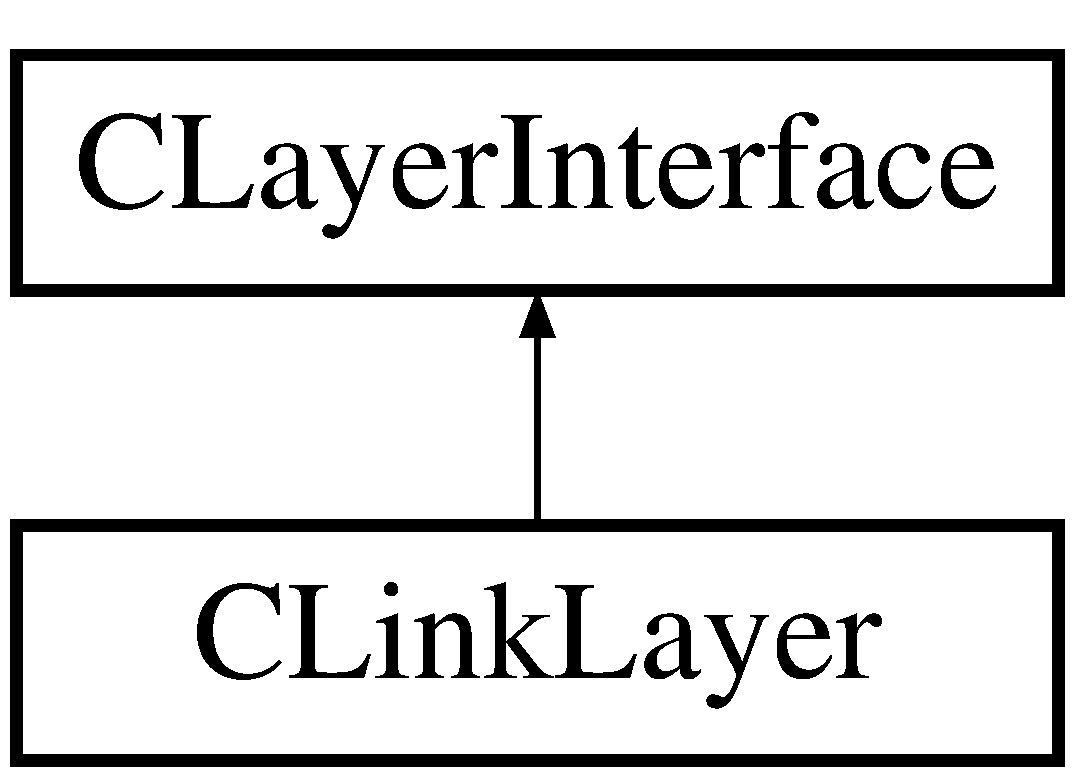
\includegraphics[height=2.000000cm]{class_c_link_layer}
\end{center}
\end{figure}
\subsection*{Public 成员函数}
\begin{DoxyCompactItemize}
\item 
\mbox{\Hypertarget{class_c_link_layer_a74cefcec9517de56f587fb26d646d610}\label{class_c_link_layer_a74cefcec9517de56f587fb26d646d610}} 
{\bfseries C\+Link\+Layer} (\hyperlink{class_msg_list}{Msg\+List} \&send\+Buf, \hyperlink{class_msg_list}{Msg\+List} \&rcv\+Buf)
\end{DoxyCompactItemize}
\subsection*{Protected 成员函数}
\begin{DoxyCompactItemize}
\item 
\mbox{\Hypertarget{class_c_link_layer_ab6a4124af45069fefeddff784ea26e3f}\label{class_c_link_layer_ab6a4124af45069fefeddff784ea26e3f}} 
void {\bfseries send\+Transfer} ()
\item 
\mbox{\Hypertarget{class_c_link_layer_a0962e4887e1893721031309a1e49a638}\label{class_c_link_layer_a0962e4887e1893721031309a1e49a638}} 
void {\bfseries add\+Tail} ()
\item 
\mbox{\Hypertarget{class_c_link_layer_a6ef143071b324acea3cd11ef86ba850f}\label{class_c_link_layer_a6ef143071b324acea3cd11ef86ba850f}} 
void {\bfseries add\+Head} ()
\end{DoxyCompactItemize}
\subsection*{额外继承的成员函数}


该类的文档由以下文件生成\+:\begin{DoxyCompactItemize}
\item 
G\+:/华中科技大学/计卓1401/大三下/计算机网络/\+Layer\+Interface/\+Link\+Layer/Link\+Layer.\+h\item 
G\+:/华中科技大学/计卓1401/大三下/计算机网络/\+Layer\+Interface/\+Link\+Layer/Link\+Layer.\+cpp\end{DoxyCompactItemize}

\hypertarget{class_c_mail_slot}{}\section{C\+Mail\+Slot类 参考}
\label{class_c_mail_slot}\index{C\+Mail\+Slot@{C\+Mail\+Slot}}
\subsection*{Public 成员函数}
\begin{DoxyCompactItemize}
\item 
bool \hyperlink{class_c_mail_slot_abdbc8ae85a1ae1f7c7998c43b1422535}{create\+Mail\+Slot} (int id)
\begin{DoxyCompactList}\small\item\em 创建邮件槽 \end{DoxyCompactList}\item 
\mbox{\Hypertarget{class_c_mail_slot_a23a09f6261450e62570ee1314c62eb97}\label{class_c_mail_slot_a23a09f6261450e62570ee1314c62eb97}} 
bool {\bfseries open} (int id)
\item 
\mbox{\Hypertarget{class_c_mail_slot_afc370072c2ab921ba66c55d1509262ad}\label{class_c_mail_slot_afc370072c2ab921ba66c55d1509262ad}} 
bool {\bfseries close} ()
\item 
\mbox{\Hypertarget{class_c_mail_slot_a8eb1b3b7bd937365ca865d76e25a4941}\label{class_c_mail_slot_a8eb1b3b7bd937365ca865d76e25a4941}} 
bool {\bfseries read} (\hyperlink{class_c_net_conn}{C\+Net\+Conn} \&conn)
\item 
\mbox{\Hypertarget{class_c_mail_slot_a17b53bd1601b38ba99bac0dda7ac0794}\label{class_c_mail_slot_a17b53bd1601b38ba99bac0dda7ac0794}} 
bool {\bfseries read} (char $\ast$\&msg, int \&length)
\item 
\mbox{\Hypertarget{class_c_mail_slot_a5eb6d0ece129a9c023cd058f45653427}\label{class_c_mail_slot_a5eb6d0ece129a9c023cd058f45653427}} 
bool {\bfseries write} (const \hyperlink{class_c_net_conn}{C\+Net\+Conn} \&conn)
\item 
\mbox{\Hypertarget{class_c_mail_slot_add3c2a84d9d2e588f23e009c08c0ca2d}\label{class_c_mail_slot_add3c2a84d9d2e588f23e009c08c0ca2d}} 
bool {\bfseries write} (const char $\ast$msg, const int length)
\item 
bool \hyperlink{class_c_mail_slot_abdbc8ae85a1ae1f7c7998c43b1422535}{create\+Mail\+Slot} (int id)
\begin{DoxyCompactList}\small\item\em 创建邮件槽 \end{DoxyCompactList}\item 
\mbox{\Hypertarget{class_c_mail_slot_a23a09f6261450e62570ee1314c62eb97}\label{class_c_mail_slot_a23a09f6261450e62570ee1314c62eb97}} 
bool {\bfseries open} (int id)
\item 
\mbox{\Hypertarget{class_c_mail_slot_afc370072c2ab921ba66c55d1509262ad}\label{class_c_mail_slot_afc370072c2ab921ba66c55d1509262ad}} 
bool {\bfseries close} ()
\item 
\mbox{\Hypertarget{class_c_mail_slot_a8eb1b3b7bd937365ca865d76e25a4941}\label{class_c_mail_slot_a8eb1b3b7bd937365ca865d76e25a4941}} 
bool {\bfseries read} (\hyperlink{class_c_net_conn}{C\+Net\+Conn} \&conn)
\item 
\mbox{\Hypertarget{class_c_mail_slot_a17b53bd1601b38ba99bac0dda7ac0794}\label{class_c_mail_slot_a17b53bd1601b38ba99bac0dda7ac0794}} 
bool {\bfseries read} (char $\ast$\&msg, int \&length)
\item 
\mbox{\Hypertarget{class_c_mail_slot_a5eb6d0ece129a9c023cd058f45653427}\label{class_c_mail_slot_a5eb6d0ece129a9c023cd058f45653427}} 
bool {\bfseries write} (const \hyperlink{class_c_net_conn}{C\+Net\+Conn} \&conn)
\item 
\mbox{\Hypertarget{class_c_mail_slot_add3c2a84d9d2e588f23e009c08c0ca2d}\label{class_c_mail_slot_add3c2a84d9d2e588f23e009c08c0ca2d}} 
bool {\bfseries write} (const char $\ast$msg, const int length)
\end{DoxyCompactItemize}
\subsection*{Public 属性}
\begin{DoxyCompactItemize}
\item 
\mbox{\Hypertarget{class_c_mail_slot_a4e3521651dae10b64456ad61b2612009}\label{class_c_mail_slot_a4e3521651dae10b64456ad61b2612009}} 
std\+::string {\bfseries last\+Err}
\end{DoxyCompactItemize}


\subsection{成员函数说明}
\mbox{\Hypertarget{class_c_mail_slot_abdbc8ae85a1ae1f7c7998c43b1422535}\label{class_c_mail_slot_abdbc8ae85a1ae1f7c7998c43b1422535}} 
\index{C\+Mail\+Slot@{C\+Mail\+Slot}!create\+Mail\+Slot@{create\+Mail\+Slot}}
\index{create\+Mail\+Slot@{create\+Mail\+Slot}!C\+Mail\+Slot@{C\+Mail\+Slot}}
\subsubsection{\texorpdfstring{create\+Mail\+Slot()}{createMailSlot()}\hspace{0.1cm}{\footnotesize\ttfamily [1/2]}}
{\footnotesize\ttfamily bool C\+Mail\+Slot\+::create\+Mail\+Slot (\begin{DoxyParamCaption}\item[{int}]{id }\end{DoxyParamCaption})}



创建邮件槽 


\begin{DoxyParams}[1]{参数}
\mbox{\tt in}  & {\em slot\+Name} & 邮件槽名字 \\
\hline
\mbox{\tt in}  & {\em socket\+Id} & socket号 \\
\hline
\end{DoxyParams}
\mbox{\Hypertarget{class_c_mail_slot_abdbc8ae85a1ae1f7c7998c43b1422535}\label{class_c_mail_slot_abdbc8ae85a1ae1f7c7998c43b1422535}} 
\index{C\+Mail\+Slot@{C\+Mail\+Slot}!create\+Mail\+Slot@{create\+Mail\+Slot}}
\index{create\+Mail\+Slot@{create\+Mail\+Slot}!C\+Mail\+Slot@{C\+Mail\+Slot}}
\subsubsection{\texorpdfstring{create\+Mail\+Slot()}{createMailSlot()}\hspace{0.1cm}{\footnotesize\ttfamily [2/2]}}
{\footnotesize\ttfamily bool C\+Mail\+Slot\+::create\+Mail\+Slot (\begin{DoxyParamCaption}\item[{int}]{id }\end{DoxyParamCaption})}



创建邮件槽 


\begin{DoxyParams}[1]{参数}
\mbox{\tt in}  & {\em slot\+Name} & 邮件槽名字 \\
\hline
\mbox{\tt in}  & {\em socket\+Id} & socket号 \\
\hline
\end{DoxyParams}


该类的文档由以下文件生成\+:\begin{DoxyCompactItemize}
\item 
G\+:/华中科技大学/计卓1401/大三下/计算机网络/\+Layer\+Interface/\+Layer\+Interface/Mail\+Slot.\+h\item 
G\+:/华中科技大学/计卓1401/大三下/计算机网络/\+Layer\+Interface/\+Layer\+Interface/Mail\+Slot.\+cpp\end{DoxyCompactItemize}

\hypertarget{class_c_n_a_t_proto}{}\section{C\+N\+A\+T\+Proto类 参考}
\label{class_c_n_a_t_proto}\index{C\+N\+A\+T\+Proto@{C\+N\+A\+T\+Proto}}


{\ttfamily \#include $<$N\+A\+T\+Proto.\+h$>$}

\subsection*{Public 成员函数}
\begin{DoxyCompactItemize}
\item 
\hyperlink{class_c_n_a_t_proto_a196de69028f8ed5b6a16bd439e07273d}{C\+N\+A\+T\+Proto} ()
\item 
\hyperlink{class_c_n_a_t_proto_a61d0e52fb1019c3b505ef28c5c7664f4}{$\sim$\+C\+N\+A\+T\+Proto} ()
\item 
void \hyperlink{class_c_n_a_t_proto_a249f93030dfaa686dfffb0f785658ca4}{convert} ()
\end{DoxyCompactItemize}
\subsection*{Public 属性}
\begin{DoxyCompactItemize}
\item 
\hyperlink{class_c_trans_table}{C\+Trans\+Table} \hyperlink{class_c_n_a_t_proto_a7fde6c1c8e6840ae207f305e85288668}{table}
\end{DoxyCompactItemize}


\subsection{详细描述}


在文件 N\+A\+T\+Proto.\+h 第 12 行定义.



\subsection{构造及析构函数说明}
\mbox{\Hypertarget{class_c_n_a_t_proto_a196de69028f8ed5b6a16bd439e07273d}\label{class_c_n_a_t_proto_a196de69028f8ed5b6a16bd439e07273d}} 
\index{C\+N\+A\+T\+Proto@{C\+N\+A\+T\+Proto}!C\+N\+A\+T\+Proto@{C\+N\+A\+T\+Proto}}
\index{C\+N\+A\+T\+Proto@{C\+N\+A\+T\+Proto}!C\+N\+A\+T\+Proto@{C\+N\+A\+T\+Proto}}
\subsubsection{\texorpdfstring{C\+N\+A\+T\+Proto()}{CNATProto()}}
{\footnotesize\ttfamily C\+N\+A\+T\+Proto\+::\+C\+N\+A\+T\+Proto (\begin{DoxyParamCaption}{ }\end{DoxyParamCaption})}



在文件 N\+A\+T\+Proto.\+cpp 第 5 行定义.

\mbox{\Hypertarget{class_c_n_a_t_proto_a61d0e52fb1019c3b505ef28c5c7664f4}\label{class_c_n_a_t_proto_a61d0e52fb1019c3b505ef28c5c7664f4}} 
\index{C\+N\+A\+T\+Proto@{C\+N\+A\+T\+Proto}!````~C\+N\+A\+T\+Proto@{$\sim$\+C\+N\+A\+T\+Proto}}
\index{````~C\+N\+A\+T\+Proto@{$\sim$\+C\+N\+A\+T\+Proto}!C\+N\+A\+T\+Proto@{C\+N\+A\+T\+Proto}}
\subsubsection{\texorpdfstring{$\sim$\+C\+N\+A\+T\+Proto()}{~CNATProto()}}
{\footnotesize\ttfamily C\+N\+A\+T\+Proto\+::$\sim$\+C\+N\+A\+T\+Proto (\begin{DoxyParamCaption}{ }\end{DoxyParamCaption})}



在文件 N\+A\+T\+Proto.\+cpp 第 10 行定义.



\subsection{成员函数说明}
\mbox{\Hypertarget{class_c_n_a_t_proto_a249f93030dfaa686dfffb0f785658ca4}\label{class_c_n_a_t_proto_a249f93030dfaa686dfffb0f785658ca4}} 
\index{C\+N\+A\+T\+Proto@{C\+N\+A\+T\+Proto}!convert@{convert}}
\index{convert@{convert}!C\+N\+A\+T\+Proto@{C\+N\+A\+T\+Proto}}
\subsubsection{\texorpdfstring{convert()}{convert()}}
{\footnotesize\ttfamily void C\+N\+A\+T\+Proto\+::convert (\begin{DoxyParamCaption}{ }\end{DoxyParamCaption})}



在文件 N\+A\+T\+Proto.\+cpp 第 15 行定义.



\subsection{类成员变量说明}
\mbox{\Hypertarget{class_c_n_a_t_proto_a7fde6c1c8e6840ae207f305e85288668}\label{class_c_n_a_t_proto_a7fde6c1c8e6840ae207f305e85288668}} 
\index{C\+N\+A\+T\+Proto@{C\+N\+A\+T\+Proto}!table@{table}}
\index{table@{table}!C\+N\+A\+T\+Proto@{C\+N\+A\+T\+Proto}}
\subsubsection{\texorpdfstring{table}{table}}
{\footnotesize\ttfamily \hyperlink{class_c_trans_table}{C\+Trans\+Table} C\+N\+A\+T\+Proto\+::table}



在文件 N\+A\+T\+Proto.\+h 第 20 行定义.



该类的文档由以下文件生成\+:\begin{DoxyCompactItemize}
\item 
G\+:/华中科技大学/计卓1401/大三下/计算机网络/\+Layer\+Interface/\+I\+P\+Layer/\hyperlink{_n_a_t_proto_8h}{N\+A\+T\+Proto.\+h}\item 
G\+:/华中科技大学/计卓1401/大三下/计算机网络/\+Layer\+Interface/\+I\+P\+Layer/\hyperlink{_n_a_t_proto_8cpp}{N\+A\+T\+Proto.\+cpp}\end{DoxyCompactItemize}

\hypertarget{class_c_net_conn}{}\section{C\+Net\+Conn类 参考}
\label{class_c_net_conn}\index{C\+Net\+Conn@{C\+Net\+Conn}}


{\ttfamily \#include $<$Net\+Conn.\+h$>$}

\subsection*{Public 成员函数}
\begin{DoxyCompactItemize}
\item 
\mbox{\Hypertarget{class_c_net_conn_acbae5bdb550ed916cfaedf6ec0caa8de}\label{class_c_net_conn_acbae5bdb550ed916cfaedf6ec0caa8de}} 
void {\bfseries alloc} (int type, int proto)
\item 
\mbox{\Hypertarget{class_c_net_conn_a9157b83f4f5d149487dadba775e53fa3}\label{class_c_net_conn_a9157b83f4f5d149487dadba775e53fa3}} 
void {\bfseries set\+Address} (std\+::string IP, unsigned int port, int is\+Remote)
\item 
\mbox{\Hypertarget{class_c_net_conn_acbae5bdb550ed916cfaedf6ec0caa8de}\label{class_c_net_conn_acbae5bdb550ed916cfaedf6ec0caa8de}} 
void {\bfseries alloc} (int type, int proto)
\item 
\mbox{\Hypertarget{class_c_net_conn_a9157b83f4f5d149487dadba775e53fa3}\label{class_c_net_conn_a9157b83f4f5d149487dadba775e53fa3}} 
void {\bfseries set\+Address} (std\+::string IP, unsigned int port, int is\+Remote)
\end{DoxyCompactItemize}
\subsection*{Public 属性}
\begin{DoxyCompactItemize}
\item 
\mbox{\Hypertarget{class_c_net_conn_af403a1097dad68c834126c515fa76893}\label{class_c_net_conn_af403a1097dad68c834126c515fa76893}} 
std\+::string {\bfseries last\+Err}
\item 
\mbox{\Hypertarget{class_c_net_conn_a622ed64d7d62629e8ac33b1d2d0c70bc}\label{class_c_net_conn_a622ed64d7d62629e8ac33b1d2d0c70bc}} 
int {\bfseries socket}
\item 
\mbox{\Hypertarget{class_c_net_conn_ab811fe46f1f54064735438c119df692e}\label{class_c_net_conn_ab811fe46f1f54064735438c119df692e}} 
std\+::string {\bfseries src\+IP}
\item 
\mbox{\Hypertarget{class_c_net_conn_a29e8c336b1ebcdec3d1867d2c8667d88}\label{class_c_net_conn_a29e8c336b1ebcdec3d1867d2c8667d88}} 
std\+::string {\bfseries dst\+IP}
\item 
\mbox{\Hypertarget{class_c_net_conn_a01763de4d43bf8f45022ad549141ec2b}\label{class_c_net_conn_a01763de4d43bf8f45022ad549141ec2b}} 
unsigned int {\bfseries src\+Port}
\item 
\mbox{\Hypertarget{class_c_net_conn_a3ba6e293a471292e135c20706d388b9c}\label{class_c_net_conn_a3ba6e293a471292e135c20706d388b9c}} 
unsigned int {\bfseries dst\+Port}
\item 
\mbox{\Hypertarget{class_c_net_conn_a887c118d2000cf8bd230a8f09579b7b7}\label{class_c_net_conn_a887c118d2000cf8bd230a8f09579b7b7}} 
int {\bfseries tran\+Proto}
\item 
\mbox{\Hypertarget{class_c_net_conn_af2958082fddd86589edf11785ccc8231}\label{class_c_net_conn_af2958082fddd86589edf11785ccc8231}} 
\hyperlink{class_c_net_conn}{C\+Net\+Conn} $\ast$ {\bfseries next}
\end{DoxyCompactItemize}
\subsection*{静态 Public 属性}
\begin{DoxyCompactItemize}
\item 
\mbox{\Hypertarget{class_c_net_conn_a4d52e492a5ac410d6bf6bb0c7d2df5a9}\label{class_c_net_conn_a4d52e492a5ac410d6bf6bb0c7d2df5a9}} 
static \hyperlink{class_c_net_conn}{C\+Net\+Conn} $\ast$ {\bfseries phead} = nullptr
\end{DoxyCompactItemize}


\subsection{详细描述}
记录链接状态信息 

该类的文档由以下文件生成\+:\begin{DoxyCompactItemize}
\item 
G\+:/华中科技大学/计卓1401/大三下/计算机网络/\+Layer\+Interface/\+Layer\+Interface/Net\+Conn.\+h\item 
G\+:/华中科技大学/计卓1401/大三下/计算机网络/\+Layer\+Interface/\+Layer\+Interface/Net\+Conn.\+cpp\end{DoxyCompactItemize}

\hypertarget{class_c_o_s_f_p_route_proto}{}\section{C\+O\+S\+F\+P\+Route\+Proto类 参考}
\label{class_c_o_s_f_p_route_proto}\index{C\+O\+S\+F\+P\+Route\+Proto@{C\+O\+S\+F\+P\+Route\+Proto}}


{\ttfamily \#include $<$O\+S\+F\+P\+Route\+Proto.\+h$>$}

类 C\+O\+S\+F\+P\+Route\+Proto 继承关系图\+:\begin{figure}[H]
\begin{center}
\leavevmode
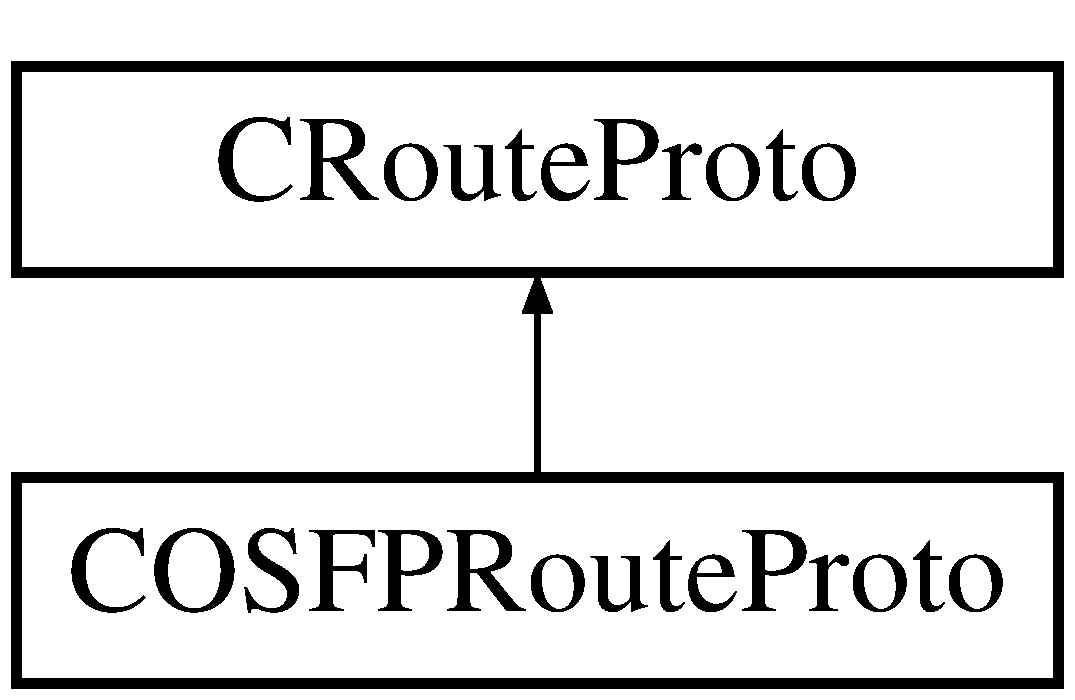
\includegraphics[height=2.000000cm]{class_c_o_s_f_p_route_proto}
\end{center}
\end{figure}
\subsection*{Public 成员函数}
\begin{DoxyCompactItemize}
\item 
\hyperlink{class_c_o_s_f_p_route_proto_a4a7e4d4d5c3c6d17fd45a1aca66c628c}{C\+O\+S\+F\+P\+Route\+Proto} (\hyperlink{class_c_i_p_layer}{C\+I\+P\+Layer} $\ast$p\+I\+P\+Proto)
\item 
\hyperlink{class_c_o_s_f_p_route_proto_a9a16b32c83097c2273bd73da0cf491da}{$\sim$\+C\+O\+S\+F\+P\+Route\+Proto} ()
\end{DoxyCompactItemize}
\subsection*{额外继承的成员函数}


\subsection{详细描述}


在文件 O\+S\+F\+P\+Route\+Proto.\+h 第 5 行定义.



\subsection{构造及析构函数说明}
\mbox{\Hypertarget{class_c_o_s_f_p_route_proto_a4a7e4d4d5c3c6d17fd45a1aca66c628c}\label{class_c_o_s_f_p_route_proto_a4a7e4d4d5c3c6d17fd45a1aca66c628c}} 
\index{C\+O\+S\+F\+P\+Route\+Proto@{C\+O\+S\+F\+P\+Route\+Proto}!C\+O\+S\+F\+P\+Route\+Proto@{C\+O\+S\+F\+P\+Route\+Proto}}
\index{C\+O\+S\+F\+P\+Route\+Proto@{C\+O\+S\+F\+P\+Route\+Proto}!C\+O\+S\+F\+P\+Route\+Proto@{C\+O\+S\+F\+P\+Route\+Proto}}
\subsubsection{\texorpdfstring{C\+O\+S\+F\+P\+Route\+Proto()}{COSFPRouteProto()}}
{\footnotesize\ttfamily C\+O\+S\+F\+P\+Route\+Proto\+::\+C\+O\+S\+F\+P\+Route\+Proto (\begin{DoxyParamCaption}\item[{\hyperlink{class_c_i_p_layer}{C\+I\+P\+Layer} $\ast$}]{p\+I\+P\+Proto }\end{DoxyParamCaption})}



在文件 O\+S\+F\+P\+Route\+Proto.\+cpp 第 5 行定义.

\mbox{\Hypertarget{class_c_o_s_f_p_route_proto_a9a16b32c83097c2273bd73da0cf491da}\label{class_c_o_s_f_p_route_proto_a9a16b32c83097c2273bd73da0cf491da}} 
\index{C\+O\+S\+F\+P\+Route\+Proto@{C\+O\+S\+F\+P\+Route\+Proto}!````~C\+O\+S\+F\+P\+Route\+Proto@{$\sim$\+C\+O\+S\+F\+P\+Route\+Proto}}
\index{````~C\+O\+S\+F\+P\+Route\+Proto@{$\sim$\+C\+O\+S\+F\+P\+Route\+Proto}!C\+O\+S\+F\+P\+Route\+Proto@{C\+O\+S\+F\+P\+Route\+Proto}}
\subsubsection{\texorpdfstring{$\sim$\+C\+O\+S\+F\+P\+Route\+Proto()}{~COSFPRouteProto()}}
{\footnotesize\ttfamily C\+O\+S\+F\+P\+Route\+Proto\+::$\sim$\+C\+O\+S\+F\+P\+Route\+Proto (\begin{DoxyParamCaption}{ }\end{DoxyParamCaption})}



在文件 O\+S\+F\+P\+Route\+Proto.\+cpp 第 10 行定义.



该类的文档由以下文件生成\+:\begin{DoxyCompactItemize}
\item 
G\+:/华中科技大学/计卓1401/大三下/计算机网络/\+Layer\+Interface/\+I\+P\+Layer/\hyperlink{_o_s_f_p_route_proto_8h}{O\+S\+F\+P\+Route\+Proto.\+h}\item 
G\+:/华中科技大学/计卓1401/大三下/计算机网络/\+Layer\+Interface/\+I\+P\+Layer/\hyperlink{_o_s_f_p_route_proto_8cpp}{O\+S\+F\+P\+Route\+Proto.\+cpp}\end{DoxyCompactItemize}

\hypertarget{class_c_p_p_p}{}\section{C\+P\+P\+P类 参考}
\label{class_c_p_p_p}\index{C\+P\+PP@{C\+P\+PP}}


{\ttfamily \#include $<$P\+P\+P.\+h$>$}

类 C\+P\+PP 继承关系图\+:\begin{figure}[H]
\begin{center}
\leavevmode
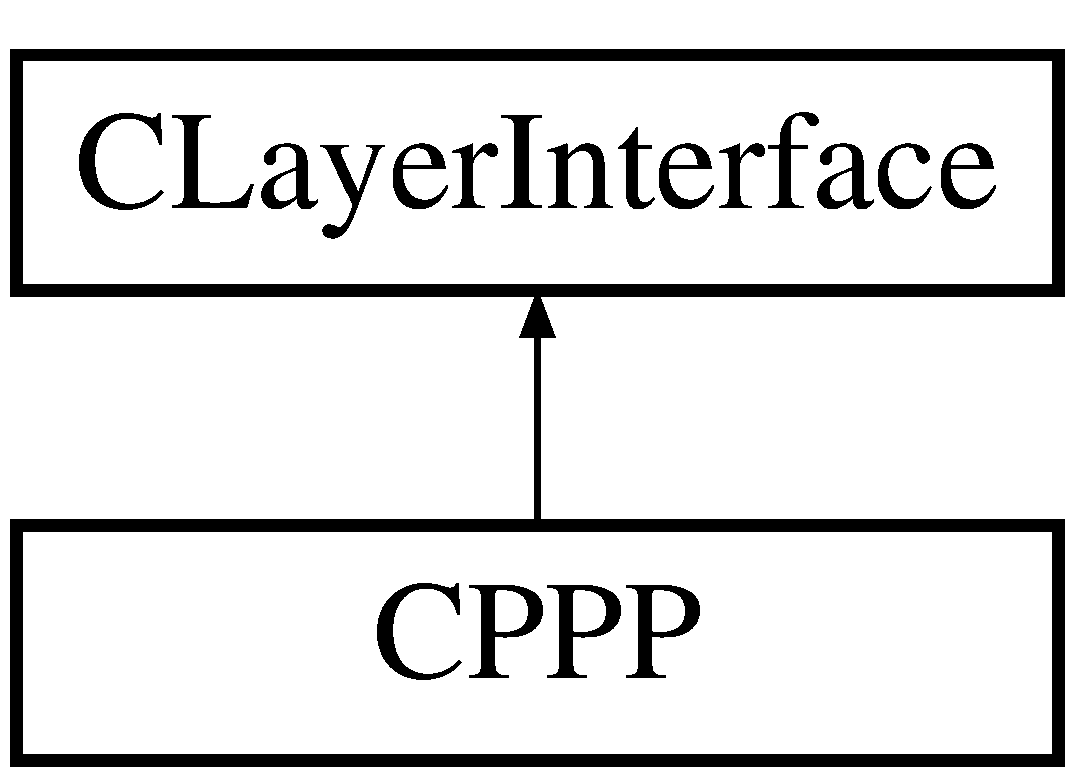
\includegraphics[height=2.000000cm]{class_c_p_p_p}
\end{center}
\end{figure}
\subsection*{Public 成员函数}
\begin{DoxyCompactItemize}
\item 
\hyperlink{class_c_p_p_p_acab476d358d55a9e8bf1618019228566}{C\+P\+PP} ()
\item 
\hyperlink{class_c_p_p_p_a27c924df735ade52f06207dcccdea395}{$\sim$\+C\+P\+PP} ()
\end{DoxyCompactItemize}
\subsection*{Protected 成员函数}
\begin{DoxyCompactItemize}
\item 
void \hyperlink{class_c_p_p_p_a1d8be0d39e44ad6e6971329106e5900d}{send\+Transfer} ()
\item 
void \hyperlink{class_c_p_p_p_a2b345908338ada3b4d9e58d14270725a}{add\+Tail} ()
\item 
void \hyperlink{class_c_p_p_p_aba6a014532e6d329cf1f8dfb591eff72}{add\+Head} ()
\end{DoxyCompactItemize}
\subsection*{额外继承的成员函数}


\subsection{详细描述}


在文件 P\+P\+P.\+h 第 8 行定义.



\subsection{构造及析构函数说明}
\mbox{\Hypertarget{class_c_p_p_p_acab476d358d55a9e8bf1618019228566}\label{class_c_p_p_p_acab476d358d55a9e8bf1618019228566}} 
\index{C\+P\+PP@{C\+P\+PP}!C\+P\+PP@{C\+P\+PP}}
\index{C\+P\+PP@{C\+P\+PP}!C\+P\+PP@{C\+P\+PP}}
\subsubsection{\texorpdfstring{C\+P\+P\+P()}{CPPP()}}
{\footnotesize\ttfamily C\+P\+P\+P\+::\+C\+P\+PP (\begin{DoxyParamCaption}{ }\end{DoxyParamCaption})}



在文件 P\+P\+P.\+cpp 第 5 行定义.

\mbox{\Hypertarget{class_c_p_p_p_a27c924df735ade52f06207dcccdea395}\label{class_c_p_p_p_a27c924df735ade52f06207dcccdea395}} 
\index{C\+P\+PP@{C\+P\+PP}!````~C\+P\+PP@{$\sim$\+C\+P\+PP}}
\index{````~C\+P\+PP@{$\sim$\+C\+P\+PP}!C\+P\+PP@{C\+P\+PP}}
\subsubsection{\texorpdfstring{$\sim$\+C\+P\+P\+P()}{~CPPP()}}
{\footnotesize\ttfamily C\+P\+P\+P\+::$\sim$\+C\+P\+PP (\begin{DoxyParamCaption}{ }\end{DoxyParamCaption})}



在文件 P\+P\+P.\+cpp 第 10 行定义.



\subsection{成员函数说明}
\mbox{\Hypertarget{class_c_p_p_p_aba6a014532e6d329cf1f8dfb591eff72}\label{class_c_p_p_p_aba6a014532e6d329cf1f8dfb591eff72}} 
\index{C\+P\+PP@{C\+P\+PP}!add\+Head@{add\+Head}}
\index{add\+Head@{add\+Head}!C\+P\+PP@{C\+P\+PP}}
\subsubsection{\texorpdfstring{add\+Head()}{addHead()}}
{\footnotesize\ttfamily void C\+P\+P\+P\+::add\+Head (\begin{DoxyParamCaption}{ }\end{DoxyParamCaption})\hspace{0.3cm}{\ttfamily [protected]}, {\ttfamily [virtual]}}



重载 \hyperlink{class_c_layer_interface_ac38c51660960657ac42e37a19ea062b4}{C\+Layer\+Interface} .



在文件 P\+P\+P.\+cpp 第 16 行定义.

\mbox{\Hypertarget{class_c_p_p_p_a2b345908338ada3b4d9e58d14270725a}\label{class_c_p_p_p_a2b345908338ada3b4d9e58d14270725a}} 
\index{C\+P\+PP@{C\+P\+PP}!add\+Tail@{add\+Tail}}
\index{add\+Tail@{add\+Tail}!C\+P\+PP@{C\+P\+PP}}
\subsubsection{\texorpdfstring{add\+Tail()}{addTail()}}
{\footnotesize\ttfamily void C\+P\+P\+P\+::add\+Tail (\begin{DoxyParamCaption}{ }\end{DoxyParamCaption})\hspace{0.3cm}{\ttfamily [protected]}, {\ttfamily [virtual]}}



重载 \hyperlink{class_c_layer_interface_a433a6f3322355291bbfc2b97343d493f}{C\+Layer\+Interface} .



在文件 P\+P\+P.\+cpp 第 15 行定义.

\mbox{\Hypertarget{class_c_p_p_p_a1d8be0d39e44ad6e6971329106e5900d}\label{class_c_p_p_p_a1d8be0d39e44ad6e6971329106e5900d}} 
\index{C\+P\+PP@{C\+P\+PP}!send\+Transfer@{send\+Transfer}}
\index{send\+Transfer@{send\+Transfer}!C\+P\+PP@{C\+P\+PP}}
\subsubsection{\texorpdfstring{send\+Transfer()}{sendTransfer()}}
{\footnotesize\ttfamily void C\+P\+P\+P\+::send\+Transfer (\begin{DoxyParamCaption}{ }\end{DoxyParamCaption})\hspace{0.3cm}{\ttfamily [protected]}, {\ttfamily [virtual]}}



重载 \hyperlink{class_c_layer_interface_a02a144b97e69df2dc47149e5314cba2d}{C\+Layer\+Interface} .



在文件 P\+P\+P.\+cpp 第 14 行定义.



该类的文档由以下文件生成\+:\begin{DoxyCompactItemize}
\item 
G\+:/华中科技大学/计卓1401/大三下/计算机网络/\+Layer\+Interface/\+Link\+Layer/\hyperlink{_p_p_p_8h}{P\+P\+P.\+h}\item 
G\+:/华中科技大学/计卓1401/大三下/计算机网络/\+Layer\+Interface/\+Link\+Layer/\hyperlink{_p_p_p_8cpp}{P\+P\+P.\+cpp}\end{DoxyCompactItemize}

\hypertarget{class_c_r_d_transfer}{}\section{C\+R\+D\+Transfer类 参考}
\label{class_c_r_d_transfer}\index{C\+R\+D\+Transfer@{C\+R\+D\+Transfer}}
类 C\+R\+D\+Transfer 继承关系图\+:\begin{figure}[H]
\begin{center}
\leavevmode
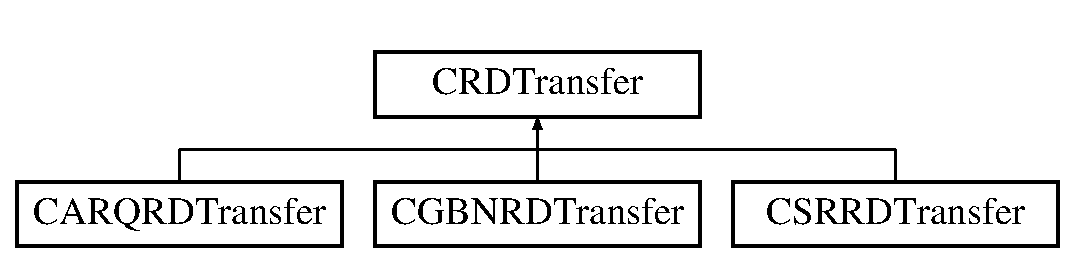
\includegraphics[height=2.000000cm]{class_c_r_d_transfer}
\end{center}
\end{figure}
\subsection*{Public 成员函数}
\begin{DoxyCompactItemize}
\item 
\mbox{\Hypertarget{class_c_r_d_transfer_ac98920ca7fa69b7d4ad47587a860e3f5}\label{class_c_r_d_transfer_ac98920ca7fa69b7d4ad47587a860e3f5}} 
void {\bfseries send} (char $\ast$p\+Datagram)
\item 
\mbox{\Hypertarget{class_c_r_d_transfer_ae2d67458270389e3eef329bbdfac8a7a}\label{class_c_r_d_transfer_ae2d67458270389e3eef329bbdfac8a7a}} 
void {\bfseries recieve} ()
\item 
\mbox{\Hypertarget{class_c_r_d_transfer_a35f5c58df35d4c513e5172d41e7707e0}\label{class_c_r_d_transfer_a35f5c58df35d4c513e5172d41e7707e0}} 
void {\bfseries set\+A\+CK} ()
\end{DoxyCompactItemize}
\subsection*{Public 属性}
\begin{DoxyCompactItemize}
\item 
\mbox{\Hypertarget{class_c_r_d_transfer_a0ea73d394ba8b738de5d151b22425be6}\label{class_c_r_d_transfer_a0ea73d394ba8b738de5d151b22425be6}} 
char $\ast$ {\bfseries m\+\_\+p\+Datagram}
\item 
\mbox{\Hypertarget{class_c_r_d_transfer_a738fa552807680744a202da502ec61fa}\label{class_c_r_d_transfer_a738fa552807680744a202da502ec61fa}} 
\hyperlink{class_c_layer_interface}{C\+Layer\+Interface} $\ast$ {\bfseries m\+\_\+p\+C\+T\+CP}
\end{DoxyCompactItemize}


该类的文档由以下文件生成\+:\begin{DoxyCompactItemize}
\item 
G\+:/华中科技大学/计卓1401/大三下/计算机网络/\+Layer\+Interface/\+T\+C\+P\+Layer/R\+D\+Transfer.\+h\item 
G\+:/华中科技大学/计卓1401/大三下/计算机网络/\+Layer\+Interface/\+T\+C\+P\+Layer/R\+D\+Transfer.\+cpp\end{DoxyCompactItemize}

\hypertarget{class_c_retransmission}{}\section{C\+Retransmission类 参考}
\label{class_c_retransmission}\index{C\+Retransmission@{C\+Retransmission}}


{\ttfamily \#include $<$Retransmission.\+h$>$}

类 C\+Retransmission 继承关系图\+:\begin{figure}[H]
\begin{center}
\leavevmode
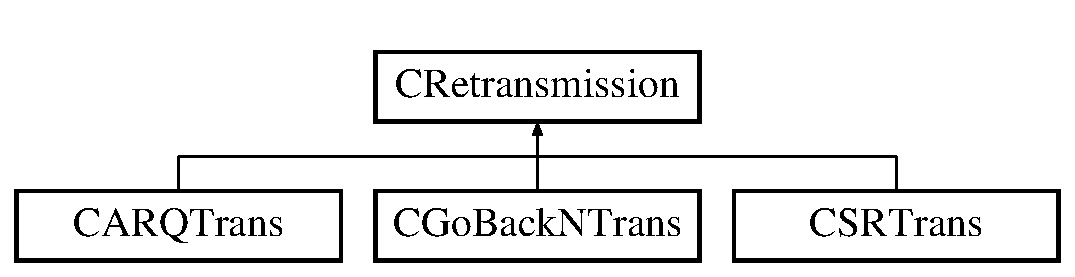
\includegraphics[height=2.000000cm]{class_c_retransmission}
\end{center}
\end{figure}
\subsection*{Public 成员函数}
\begin{DoxyCompactItemize}
\item 
\hyperlink{class_c_retransmission_a2246d5c5771f33f315bbbc1ec6e36685}{C\+Retransmission} ()
\item 
\hyperlink{class_c_retransmission_aba5baf50f86cf183e780add3562dfeca}{$\sim$\+C\+Retransmission} ()
\item 
virtual void \hyperlink{class_c_retransmission_a2a97991aa1bd05adf369d0a1b38b2a10}{send} ()
\item 
virtual void \hyperlink{class_c_retransmission_afd36095dafeb4a237e0b6f7c68bb989b}{recv} ()
\end{DoxyCompactItemize}


\subsection{详细描述}


在文件 Retransmission.\+h 第 15 行定义.



\subsection{构造及析构函数说明}
\mbox{\Hypertarget{class_c_retransmission_a2246d5c5771f33f315bbbc1ec6e36685}\label{class_c_retransmission_a2246d5c5771f33f315bbbc1ec6e36685}} 
\index{C\+Retransmission@{C\+Retransmission}!C\+Retransmission@{C\+Retransmission}}
\index{C\+Retransmission@{C\+Retransmission}!C\+Retransmission@{C\+Retransmission}}
\subsubsection{\texorpdfstring{C\+Retransmission()}{CRetransmission()}}
{\footnotesize\ttfamily C\+Retransmission\+::\+C\+Retransmission (\begin{DoxyParamCaption}{ }\end{DoxyParamCaption})}



在文件 Retransmission.\+cpp 第 5 行定义.

\mbox{\Hypertarget{class_c_retransmission_aba5baf50f86cf183e780add3562dfeca}\label{class_c_retransmission_aba5baf50f86cf183e780add3562dfeca}} 
\index{C\+Retransmission@{C\+Retransmission}!````~C\+Retransmission@{$\sim$\+C\+Retransmission}}
\index{````~C\+Retransmission@{$\sim$\+C\+Retransmission}!C\+Retransmission@{C\+Retransmission}}
\subsubsection{\texorpdfstring{$\sim$\+C\+Retransmission()}{~CRetransmission()}}
{\footnotesize\ttfamily C\+Retransmission\+::$\sim$\+C\+Retransmission (\begin{DoxyParamCaption}{ }\end{DoxyParamCaption})}



在文件 Retransmission.\+cpp 第 10 行定义.



\subsection{成员函数说明}
\mbox{\Hypertarget{class_c_retransmission_afd36095dafeb4a237e0b6f7c68bb989b}\label{class_c_retransmission_afd36095dafeb4a237e0b6f7c68bb989b}} 
\index{C\+Retransmission@{C\+Retransmission}!recv@{recv}}
\index{recv@{recv}!C\+Retransmission@{C\+Retransmission}}
\subsubsection{\texorpdfstring{recv()}{recv()}}
{\footnotesize\ttfamily void C\+Retransmission\+::recv (\begin{DoxyParamCaption}{ }\end{DoxyParamCaption})\hspace{0.3cm}{\ttfamily [virtual]}}



在文件 Retransmission.\+cpp 第 19 行定义.

\mbox{\Hypertarget{class_c_retransmission_a2a97991aa1bd05adf369d0a1b38b2a10}\label{class_c_retransmission_a2a97991aa1bd05adf369d0a1b38b2a10}} 
\index{C\+Retransmission@{C\+Retransmission}!send@{send}}
\index{send@{send}!C\+Retransmission@{C\+Retransmission}}
\subsubsection{\texorpdfstring{send()}{send()}}
{\footnotesize\ttfamily void C\+Retransmission\+::send (\begin{DoxyParamCaption}{ }\end{DoxyParamCaption})\hspace{0.3cm}{\ttfamily [virtual]}}



在文件 Retransmission.\+cpp 第 14 行定义.



该类的文档由以下文件生成\+:\begin{DoxyCompactItemize}
\item 
G\+:/华中科技大学/计卓1401/大三下/计算机网络/\+Layer\+Interface/\+Transport\+Layer/\hyperlink{_retransmission_8h}{Retransmission.\+h}\item 
G\+:/华中科技大学/计卓1401/大三下/计算机网络/\+Layer\+Interface/\+Transport\+Layer/\hyperlink{_retransmission_8cpp}{Retransmission.\+cpp}\end{DoxyCompactItemize}

\hypertarget{class_c_r_i_p_route_proto}{}\section{C\+R\+I\+P\+Route\+Proto类 参考}
\label{class_c_r_i_p_route_proto}\index{C\+R\+I\+P\+Route\+Proto@{C\+R\+I\+P\+Route\+Proto}}
类 C\+R\+I\+P\+Route\+Proto 继承关系图\+:\begin{figure}[H]
\begin{center}
\leavevmode
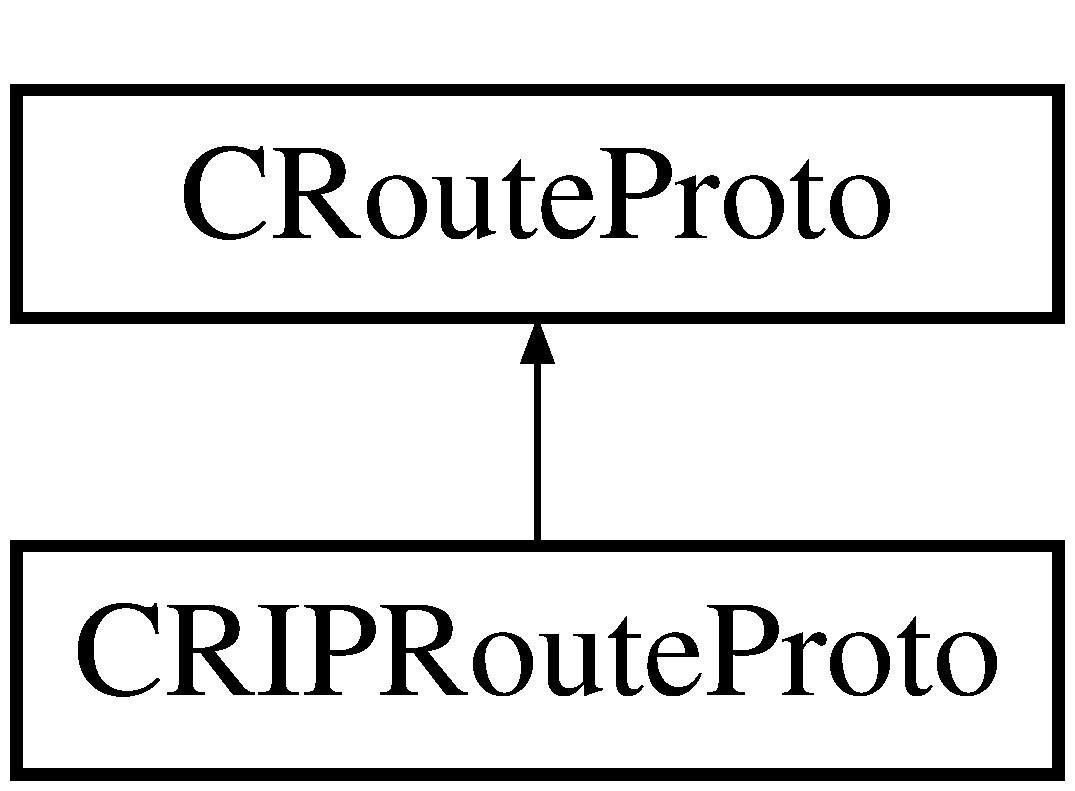
\includegraphics[height=2.000000cm]{class_c_r_i_p_route_proto}
\end{center}
\end{figure}
\subsection*{Public 成员函数}
\begin{DoxyCompactItemize}
\item 
\mbox{\Hypertarget{class_c_r_i_p_route_proto_a75e098dbb570322ad14aba1ea6e06adb}\label{class_c_r_i_p_route_proto_a75e098dbb570322ad14aba1ea6e06adb}} 
{\bfseries C\+R\+I\+P\+Route\+Proto} (\hyperlink{class_c_i_p_layer}{C\+I\+P\+Layer} $\ast$p\+I\+P\+Proto)
\end{DoxyCompactItemize}
\subsection*{额外继承的成员函数}


该类的文档由以下文件生成\+:\begin{DoxyCompactItemize}
\item 
G\+:/华中科技大学/计卓1401/大三下/计算机网络/\+Layer\+Interface/\+I\+P\+Layer/R\+I\+P\+Route\+Proto.\+h\item 
G\+:/华中科技大学/计卓1401/大三下/计算机网络/\+Layer\+Interface/\+I\+P\+Layer/R\+I\+P\+Route\+Proto.\+cpp\end{DoxyCompactItemize}

\hypertarget{class_c_route_proto}{}\section{C\+Route\+Proto类 参考}
\label{class_c_route_proto}\index{C\+Route\+Proto@{C\+Route\+Proto}}
类 C\+Route\+Proto 继承关系图\+:\begin{figure}[H]
\begin{center}
\leavevmode
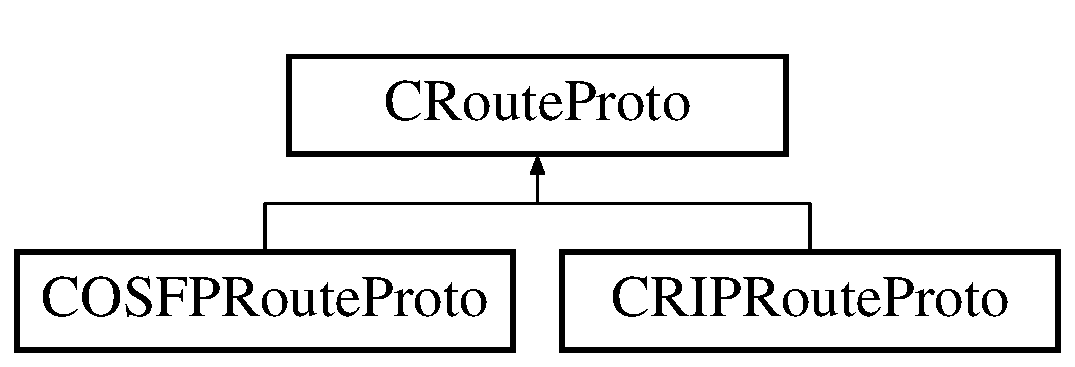
\includegraphics[height=2.000000cm]{class_c_route_proto}
\end{center}
\end{figure}
\subsection*{Public 成员函数}
\begin{DoxyCompactItemize}
\item 
\mbox{\Hypertarget{class_c_route_proto_a0af8908129d928acbadf7eba99d9b7e2}\label{class_c_route_proto_a0af8908129d928acbadf7eba99d9b7e2}} 
{\bfseries C\+Route\+Proto} (\hyperlink{class_c_i_p_layer}{C\+I\+P\+Layer} $\ast$p\+I\+P\+Proto)
\item 
\mbox{\Hypertarget{class_c_route_proto_ac17d99e82f088ed1b50426584c65b2d1}\label{class_c_route_proto_ac17d99e82f088ed1b50426584c65b2d1}} 
void {\bfseries update} ()
\end{DoxyCompactItemize}
\subsection*{Protected 属性}
\begin{DoxyCompactItemize}
\item 
\mbox{\Hypertarget{class_c_route_proto_a215ec5768c5e1c1d1350506b800f3d02}\label{class_c_route_proto_a215ec5768c5e1c1d1350506b800f3d02}} 
\hyperlink{class_c_i_p_layer}{C\+I\+P\+Layer} $\ast$ {\bfseries m\+\_\+p\+I\+P\+Proto}
\end{DoxyCompactItemize}


该类的文档由以下文件生成\+:\begin{DoxyCompactItemize}
\item 
G\+:/华中科技大学/计卓1401/大三下/计算机网络/\+Layer\+Interface/\+I\+P\+Layer/Route\+Proto.\+h\item 
G\+:/华中科技大学/计卓1401/大三下/计算机网络/\+Layer\+Interface/\+I\+P\+Layer/Route\+Proto.\+cpp\end{DoxyCompactItemize}

\hypertarget{class_c_service}{}\section{C\+Service类 参考}
\label{class_c_service}\index{C\+Service@{C\+Service}}


{\ttfamily \#include $<$Service.\+h$>$}

\subsection*{Public 类型}
\begin{DoxyCompactItemize}
\item 
enum \hyperlink{class_c_service_abd1684d960aef251b1d74edf372c5d1b}{S\+O\+C\+K\+\_\+\+P\+R\+O\+TO} \{ \hyperlink{class_c_service_abd1684d960aef251b1d74edf372c5d1ba479167516419221933e0143b80a50152}{S\+T\+R\+E\+AM} = 1, 
\hyperlink{class_c_service_abd1684d960aef251b1d74edf372c5d1bafda42db5e2e8f056a2efd03bfa0f3e96}{D\+G\+R\+AM} = 2, 
\hyperlink{class_c_service_abd1684d960aef251b1d74edf372c5d1bab25fd2485455ea631949e45849c7c390}{R\+AW} = 3
 \}
\item 
enum \hyperlink{class_c_service_a43fb60063bc9f9b0f4e3eeb1787056b0}{Proto} \{ \hyperlink{class_c_service_a43fb60063bc9f9b0f4e3eeb1787056b0a69fdc51ce4262393db36351c381d86a9}{T\+CP}, 
\hyperlink{class_c_service_a43fb60063bc9f9b0f4e3eeb1787056b0ac45d78d4edd8c6f5d27519dffc61f001}{U\+DP}
 \}
\end{DoxyCompactItemize}
\subsection*{Public 成员函数}
\begin{DoxyCompactItemize}
\item 
\hyperlink{class_c_service_ac4fb853bd01a2b0d71399ab28de19cc6}{C\+Service} (void)
\item 
int \hyperlink{class_c_service_ae632f34f3aceab829b89ee46374658f2}{socket} (int domain, int type, int protocol)
\begin{DoxyCompactList}\small\item\em 用于创建一个socket描述符,它唯一标识一个socket \end{DoxyCompactList}\item 
int \hyperlink{class_c_service_ab345d03f1f85d053472b05de3ea211eb}{bind} (int socket\+Id, std\+::string IP, unsigned short int port)
\begin{DoxyCompactList}\small\item\em 服务器绑定\+I\+P与端口号 \end{DoxyCompactList}\item 
int \hyperlink{class_c_service_a32f59bebc1aef849f38b72218a87c674}{listen} (int socket\+Id, int link\+Size)
\begin{DoxyCompactList}\small\item\em 服务器端监听 \end{DoxyCompactList}\item 
int \hyperlink{class_c_service_a4788fc741e72baeaa5e15e459494f661}{connect} (int socket\+Id, std\+::string IP, unsigned short int port)
\begin{DoxyCompactList}\small\item\em 客户端请求链接\+I\+P与端口号 \end{DoxyCompactList}\item 
int \hyperlink{class_c_service_a694c7ac8c230b0d1d11bc98a32abcd71}{accept} (int socket\+Id, std\+::string \&IP, unsigned short int \&port)
\begin{DoxyCompactList}\small\item\em 服务器同意链接 \end{DoxyCompactList}\item 
int \hyperlink{class_c_service_a221d063aa8a89ecc84084e1bbd287210}{recv} (int socket\+Id, char $\ast$\&msg, int \&length)
\begin{DoxyCompactList}\small\item\em 发送与接收 \end{DoxyCompactList}\item 
int \hyperlink{class_c_service_a883e80cc5ea699e8408bbffe7c18414b}{send} (int socket\+Id, char $\ast$msg, int length)
\item 
int \hyperlink{class_c_service_abb0357bf57a735cc27f0e667d7e21787}{close} (int socket\+Id)
\begin{DoxyCompactList}\small\item\em 关闭连接 \end{DoxyCompactList}\end{DoxyCompactItemize}


\subsection{详细描述}


在文件 Service.\+h 第 23 行定义.



\subsection{成员枚举类型说明}
\mbox{\Hypertarget{class_c_service_a43fb60063bc9f9b0f4e3eeb1787056b0}\label{class_c_service_a43fb60063bc9f9b0f4e3eeb1787056b0}} 
\index{C\+Service@{C\+Service}!Proto@{Proto}}
\index{Proto@{Proto}!C\+Service@{C\+Service}}
\subsubsection{\texorpdfstring{Proto}{Proto}}
{\footnotesize\ttfamily enum \hyperlink{class_c_service_a43fb60063bc9f9b0f4e3eeb1787056b0}{C\+Service\+::\+Proto}}

\begin{DoxyEnumFields}{枚举值}
\raisebox{\heightof{T}}[0pt][0pt]{\index{T\+CP@{T\+CP}!C\+Service@{C\+Service}}\index{C\+Service@{C\+Service}!T\+CP@{T\+CP}}}\mbox{\Hypertarget{class_c_service_a43fb60063bc9f9b0f4e3eeb1787056b0a69fdc51ce4262393db36351c381d86a9}\label{class_c_service_a43fb60063bc9f9b0f4e3eeb1787056b0a69fdc51ce4262393db36351c381d86a9}} 
T\+CP&\\
\hline

\raisebox{\heightof{T}}[0pt][0pt]{\index{U\+DP@{U\+DP}!C\+Service@{C\+Service}}\index{C\+Service@{C\+Service}!U\+DP@{U\+DP}}}\mbox{\Hypertarget{class_c_service_a43fb60063bc9f9b0f4e3eeb1787056b0ac45d78d4edd8c6f5d27519dffc61f001}\label{class_c_service_a43fb60063bc9f9b0f4e3eeb1787056b0ac45d78d4edd8c6f5d27519dffc61f001}} 
U\+DP&\\
\hline

\end{DoxyEnumFields}


在文件 Service.\+h 第 94 行定义.

\mbox{\Hypertarget{class_c_service_abd1684d960aef251b1d74edf372c5d1b}\label{class_c_service_abd1684d960aef251b1d74edf372c5d1b}} 
\index{C\+Service@{C\+Service}!S\+O\+C\+K\+\_\+\+P\+R\+O\+TO@{S\+O\+C\+K\+\_\+\+P\+R\+O\+TO}}
\index{S\+O\+C\+K\+\_\+\+P\+R\+O\+TO@{S\+O\+C\+K\+\_\+\+P\+R\+O\+TO}!C\+Service@{C\+Service}}
\subsubsection{\texorpdfstring{S\+O\+C\+K\+\_\+\+P\+R\+O\+TO}{SOCK\_PROTO}}
{\footnotesize\ttfamily enum \hyperlink{class_c_service_abd1684d960aef251b1d74edf372c5d1b}{C\+Service\+::\+S\+O\+C\+K\+\_\+\+P\+R\+O\+TO}}

\begin{DoxyEnumFields}{枚举值}
\raisebox{\heightof{T}}[0pt][0pt]{\index{S\+T\+R\+E\+AM@{S\+T\+R\+E\+AM}!C\+Service@{C\+Service}}\index{C\+Service@{C\+Service}!S\+T\+R\+E\+AM@{S\+T\+R\+E\+AM}}}\mbox{\Hypertarget{class_c_service_abd1684d960aef251b1d74edf372c5d1ba479167516419221933e0143b80a50152}\label{class_c_service_abd1684d960aef251b1d74edf372c5d1ba479167516419221933e0143b80a50152}} 
S\+T\+R\+E\+AM&\\
\hline

\raisebox{\heightof{T}}[0pt][0pt]{\index{D\+G\+R\+AM@{D\+G\+R\+AM}!C\+Service@{C\+Service}}\index{C\+Service@{C\+Service}!D\+G\+R\+AM@{D\+G\+R\+AM}}}\mbox{\Hypertarget{class_c_service_abd1684d960aef251b1d74edf372c5d1bafda42db5e2e8f056a2efd03bfa0f3e96}\label{class_c_service_abd1684d960aef251b1d74edf372c5d1bafda42db5e2e8f056a2efd03bfa0f3e96}} 
D\+G\+R\+AM&\\
\hline

\raisebox{\heightof{T}}[0pt][0pt]{\index{R\+AW@{R\+AW}!C\+Service@{C\+Service}}\index{C\+Service@{C\+Service}!R\+AW@{R\+AW}}}\mbox{\Hypertarget{class_c_service_abd1684d960aef251b1d74edf372c5d1bab25fd2485455ea631949e45849c7c390}\label{class_c_service_abd1684d960aef251b1d74edf372c5d1bab25fd2485455ea631949e45849c7c390}} 
R\+AW&\\
\hline

\end{DoxyEnumFields}


在文件 Service.\+h 第 87 行定义.



\subsection{构造及析构函数说明}
\mbox{\Hypertarget{class_c_service_ac4fb853bd01a2b0d71399ab28de19cc6}\label{class_c_service_ac4fb853bd01a2b0d71399ab28de19cc6}} 
\index{C\+Service@{C\+Service}!C\+Service@{C\+Service}}
\index{C\+Service@{C\+Service}!C\+Service@{C\+Service}}
\subsubsection{\texorpdfstring{C\+Service()}{CService()}}
{\footnotesize\ttfamily C\+Service\+::\+C\+Service (\begin{DoxyParamCaption}\item[{void}]{ }\end{DoxyParamCaption})}



在文件 Service.\+cpp 第 22 行定义.



\subsection{成员函数说明}
\mbox{\Hypertarget{class_c_service_a694c7ac8c230b0d1d11bc98a32abcd71}\label{class_c_service_a694c7ac8c230b0d1d11bc98a32abcd71}} 
\index{C\+Service@{C\+Service}!accept@{accept}}
\index{accept@{accept}!C\+Service@{C\+Service}}
\subsubsection{\texorpdfstring{accept()}{accept()}}
{\footnotesize\ttfamily int C\+Service\+::accept (\begin{DoxyParamCaption}\item[{int}]{socket\+Id,  }\item[{std\+::string \&}]{IP,  }\item[{unsigned short int \&}]{port }\end{DoxyParamCaption})}



服务器同意链接 


\begin{DoxyParams}[1]{参数}
\mbox{\tt in}  & {\em socket\+Id} & \+: socket描述符 \\
\hline
\mbox{\tt in}  & {\em I\+P:客户端网络地址} & \\
\hline
\mbox{\tt in}  & {\em port:客户端端口号} & \\
\hline
\end{DoxyParams}
\begin{DoxyReturn}{返回}
socket描述符 
\end{DoxyReturn}


在文件 Service.\+cpp 第 89 行定义.

\mbox{\Hypertarget{class_c_service_ab345d03f1f85d053472b05de3ea211eb}\label{class_c_service_ab345d03f1f85d053472b05de3ea211eb}} 
\index{C\+Service@{C\+Service}!bind@{bind}}
\index{bind@{bind}!C\+Service@{C\+Service}}
\subsubsection{\texorpdfstring{bind()}{bind()}}
{\footnotesize\ttfamily int C\+Service\+::bind (\begin{DoxyParamCaption}\item[{int}]{socket\+Id,  }\item[{std\+::string}]{IP,  }\item[{unsigned short int}]{port }\end{DoxyParamCaption})}



服务器绑定\+I\+P与端口号 


\begin{DoxyParams}[1]{参数}
\mbox{\tt in}  & {\em socket\+Id} & \+: socket描述符 \\
\hline
\mbox{\tt in}  & {\em I\+P:网络地址} & \\
\hline
\mbox{\tt in}  & {\em port:端口号} & \\
\hline
\end{DoxyParams}
\begin{DoxyReturn}{返回}
错误码 
\end{DoxyReturn}


在文件 Service.\+cpp 第 68 行定义.

\mbox{\Hypertarget{class_c_service_abb0357bf57a735cc27f0e667d7e21787}\label{class_c_service_abb0357bf57a735cc27f0e667d7e21787}} 
\index{C\+Service@{C\+Service}!close@{close}}
\index{close@{close}!C\+Service@{C\+Service}}
\subsubsection{\texorpdfstring{close()}{close()}}
{\footnotesize\ttfamily int C\+Service\+::close (\begin{DoxyParamCaption}\item[{int}]{socket\+Id }\end{DoxyParamCaption})}



关闭连接 


\begin{DoxyParams}[1]{参数}
\mbox{\tt in}  & {\em socket\+Id} & \+: socket描述符 \\
\hline
\end{DoxyParams}
\begin{DoxyReturn}{返回}
socket描述符 
\end{DoxyReturn}


在文件 Service.\+cpp 第 127 行定义.

\mbox{\Hypertarget{class_c_service_a4788fc741e72baeaa5e15e459494f661}\label{class_c_service_a4788fc741e72baeaa5e15e459494f661}} 
\index{C\+Service@{C\+Service}!connect@{connect}}
\index{connect@{connect}!C\+Service@{C\+Service}}
\subsubsection{\texorpdfstring{connect()}{connect()}}
{\footnotesize\ttfamily int C\+Service\+::connect (\begin{DoxyParamCaption}\item[{int}]{socket\+Id,  }\item[{std\+::string}]{IP,  }\item[{unsigned short int}]{port }\end{DoxyParamCaption})}



客户端请求链接\+I\+P与端口号 


\begin{DoxyParams}[1]{参数}
\mbox{\tt in}  & {\em socket\+Id} & \+: socket描述符 \\
\hline
\mbox{\tt in}  & {\em I\+P:网络地址} & \\
\hline
\mbox{\tt in}  & {\em port:端口号} & \\
\hline
\end{DoxyParams}
\begin{DoxyReturn}{返回}
错误码 
\end{DoxyReturn}


在文件 Service.\+cpp 第 73 行定义.

\mbox{\Hypertarget{class_c_service_a32f59bebc1aef849f38b72218a87c674}\label{class_c_service_a32f59bebc1aef849f38b72218a87c674}} 
\index{C\+Service@{C\+Service}!listen@{listen}}
\index{listen@{listen}!C\+Service@{C\+Service}}
\subsubsection{\texorpdfstring{listen()}{listen()}}
{\footnotesize\ttfamily int C\+Service\+::listen (\begin{DoxyParamCaption}\item[{int}]{socket\+Id,  }\item[{int}]{link\+Size }\end{DoxyParamCaption})}



服务器端监听 


\begin{DoxyParams}[1]{参数}
\mbox{\tt in}  & {\em socket\+Id} & \+: socket描述符 \\
\hline
\mbox{\tt in}  & {\em link\+Size} & \+: socket可以排队的最大连接个数 \\
\hline
\end{DoxyParams}
\begin{DoxyReturn}{返回}
错误码 
\end{DoxyReturn}


在文件 Service.\+cpp 第 84 行定义.

\mbox{\Hypertarget{class_c_service_a221d063aa8a89ecc84084e1bbd287210}\label{class_c_service_a221d063aa8a89ecc84084e1bbd287210}} 
\index{C\+Service@{C\+Service}!recv@{recv}}
\index{recv@{recv}!C\+Service@{C\+Service}}
\subsubsection{\texorpdfstring{recv()}{recv()}}
{\footnotesize\ttfamily int C\+Service\+::recv (\begin{DoxyParamCaption}\item[{int}]{socket\+Id,  }\item[{char $\ast$\&}]{msg,  }\item[{int \&}]{length }\end{DoxyParamCaption})}



发送与接收 



在文件 Service.\+cpp 第 94 行定义.

\mbox{\Hypertarget{class_c_service_a883e80cc5ea699e8408bbffe7c18414b}\label{class_c_service_a883e80cc5ea699e8408bbffe7c18414b}} 
\index{C\+Service@{C\+Service}!send@{send}}
\index{send@{send}!C\+Service@{C\+Service}}
\subsubsection{\texorpdfstring{send()}{send()}}
{\footnotesize\ttfamily int C\+Service\+::send (\begin{DoxyParamCaption}\item[{int}]{socket\+Id,  }\item[{char $\ast$}]{msg,  }\item[{int}]{length }\end{DoxyParamCaption})}



在文件 Service.\+cpp 第 104 行定义.

\mbox{\Hypertarget{class_c_service_ae632f34f3aceab829b89ee46374658f2}\label{class_c_service_ae632f34f3aceab829b89ee46374658f2}} 
\index{C\+Service@{C\+Service}!socket@{socket}}
\index{socket@{socket}!C\+Service@{C\+Service}}
\subsubsection{\texorpdfstring{socket()}{socket()}}
{\footnotesize\ttfamily int C\+Service\+::socket (\begin{DoxyParamCaption}\item[{int}]{domain,  }\item[{int}]{type,  }\item[{int}]{protocol }\end{DoxyParamCaption})}



用于创建一个socket描述符,它唯一标识一个socket 


\begin{DoxyParams}[1]{参数}
\mbox{\tt in}  & {\em domain:即协议域,又称为协议族} & \\
\hline
\mbox{\tt in}  & {\em type:指定socket类型} & \\
\hline
\mbox{\tt in}  & {\em protocol:指定协议} & \\
\hline
\end{DoxyParams}
\begin{DoxyReturn}{返回}
socket标识符 
\end{DoxyReturn}


在文件 Service.\+cpp 第 30 行定义.



该类的文档由以下文件生成\+:\begin{DoxyCompactItemize}
\item 
G\+:/华中科技大学/计卓1401/大三下/计算机网络/\+Layer\+Interface/\+Service/\hyperlink{_service_8h}{Service.\+h}\item 
G\+:/华中科技大学/计卓1401/大三下/计算机网络/\+Layer\+Interface/\+Service/\hyperlink{_service_8cpp}{Service.\+cpp}\end{DoxyCompactItemize}

\hypertarget{class_c_socket}{}\section{C\+Socket类 参考}
\label{class_c_socket}\index{C\+Socket@{C\+Socket}}


{\ttfamily \#include $<$Socket.\+h$>$}

\subsection*{Public 类型}
\begin{DoxyCompactItemize}
\item 
enum \hyperlink{class_c_socket_a1612592be6a8334d298c6e289b7d4ac7}{S\+O\+C\+K\+\_\+\+P\+R\+O\+TO} \{ \hyperlink{class_c_socket_a1612592be6a8334d298c6e289b7d4ac7aa68b727cc96993e7b2d851efc206b816}{S\+T\+R\+E\+AM} = 1, 
\hyperlink{class_c_socket_a1612592be6a8334d298c6e289b7d4ac7ae4111634fb817bbe019d43d5466d4684}{D\+G\+R\+AM} = 2, 
\hyperlink{class_c_socket_a1612592be6a8334d298c6e289b7d4ac7abcc2f37504b085d7d179861968a81bfd}{R\+AW} = 3
 \}
\item 
enum \hyperlink{class_c_socket_a9f5168b936eacaffc83a9ba3200ec00b}{Proto} \{ \hyperlink{class_c_socket_a9f5168b936eacaffc83a9ba3200ec00ba2896b183058aba44c8b256aba6e04ede}{T\+CP}, 
\hyperlink{class_c_socket_a9f5168b936eacaffc83a9ba3200ec00baf8434cb3900ac44e8898d5e430b34e2c}{U\+DP}
 \}
\end{DoxyCompactItemize}
\subsection*{Public 成员函数}
\begin{DoxyCompactItemize}
\item 
\hyperlink{class_c_socket_a3f5f8efaa44309a1991e72b985a49a33}{C\+Socket} ()
\item 
int \hyperlink{class_c_socket_abc15c93dfbf879f5dacc8b4b5dd951b1}{socket} (int domain, int type, int protocol)
\begin{DoxyCompactList}\small\item\em 用于创建一个socket描述符,它唯一标识一个socket \end{DoxyCompactList}\item 
int \hyperlink{class_c_socket_a498e08712781a360f2cb2279bd1151c4}{bind} (int socket\+Id, std\+::string IP, unsigned short int port)
\begin{DoxyCompactList}\small\item\em 服务器绑定\+I\+P与端口号 \end{DoxyCompactList}\item 
int \hyperlink{class_c_socket_acfbd568b041bb6ac35c5fc862aee28f1}{listen} (int socket\+Id, int link\+Size)
\begin{DoxyCompactList}\small\item\em 服务器端监听 \end{DoxyCompactList}\item 
int \hyperlink{class_c_socket_a7c54f8c3c1fef6dd1c84c105e99ddbb1}{connect} (int socket\+Id, std\+::string IP, unsigned short int port)
\begin{DoxyCompactList}\small\item\em 客户端请求链接\+I\+P与端口号 \end{DoxyCompactList}\item 
int \hyperlink{class_c_socket_aaf0c338bcac7bbb4b9a4e57f62c7e7df}{accept} (int socket\+Id, std\+::string \&IP, unsigned short int \&port)
\begin{DoxyCompactList}\small\item\em 服务器同意链接 \end{DoxyCompactList}\item 
int \hyperlink{class_c_socket_aafbbf6818bd94b8fda58b8a7ee8417c3}{recv} (int socket\+Id, char $\ast$\&msg, int \&length)
\begin{DoxyCompactList}\small\item\em 发送与接收 \end{DoxyCompactList}\item 
int \hyperlink{class_c_socket_ab034dd0ed69981237cc8385a6786d5ab}{send} (int socket\+Id, char $\ast$msg, int length)
\item 
int \hyperlink{class_c_socket_a1af720c8b15569d9f8f6abd91bc1bfe7}{close} (int socket\+Id)
\begin{DoxyCompactList}\small\item\em 关闭连接 \end{DoxyCompactList}\end{DoxyCompactItemize}


\subsection{详细描述}


在文件 Socket.\+h 第 6 行定义.



\subsection{成员枚举类型说明}
\mbox{\Hypertarget{class_c_socket_a9f5168b936eacaffc83a9ba3200ec00b}\label{class_c_socket_a9f5168b936eacaffc83a9ba3200ec00b}} 
\index{C\+Socket@{C\+Socket}!Proto@{Proto}}
\index{Proto@{Proto}!C\+Socket@{C\+Socket}}
\subsubsection{\texorpdfstring{Proto}{Proto}}
{\footnotesize\ttfamily enum \hyperlink{class_c_socket_a9f5168b936eacaffc83a9ba3200ec00b}{C\+Socket\+::\+Proto}}

\begin{DoxyEnumFields}{枚举值}
\raisebox{\heightof{T}}[0pt][0pt]{\index{T\+CP@{T\+CP}!C\+Socket@{C\+Socket}}\index{C\+Socket@{C\+Socket}!T\+CP@{T\+CP}}}\mbox{\Hypertarget{class_c_socket_a9f5168b936eacaffc83a9ba3200ec00ba2896b183058aba44c8b256aba6e04ede}\label{class_c_socket_a9f5168b936eacaffc83a9ba3200ec00ba2896b183058aba44c8b256aba6e04ede}} 
T\+CP&\\
\hline

\raisebox{\heightof{T}}[0pt][0pt]{\index{U\+DP@{U\+DP}!C\+Socket@{C\+Socket}}\index{C\+Socket@{C\+Socket}!U\+DP@{U\+DP}}}\mbox{\Hypertarget{class_c_socket_a9f5168b936eacaffc83a9ba3200ec00baf8434cb3900ac44e8898d5e430b34e2c}\label{class_c_socket_a9f5168b936eacaffc83a9ba3200ec00baf8434cb3900ac44e8898d5e430b34e2c}} 
U\+DP&\\
\hline

\end{DoxyEnumFields}


在文件 Socket.\+h 第 76 行定义.

\mbox{\Hypertarget{class_c_socket_a1612592be6a8334d298c6e289b7d4ac7}\label{class_c_socket_a1612592be6a8334d298c6e289b7d4ac7}} 
\index{C\+Socket@{C\+Socket}!S\+O\+C\+K\+\_\+\+P\+R\+O\+TO@{S\+O\+C\+K\+\_\+\+P\+R\+O\+TO}}
\index{S\+O\+C\+K\+\_\+\+P\+R\+O\+TO@{S\+O\+C\+K\+\_\+\+P\+R\+O\+TO}!C\+Socket@{C\+Socket}}
\subsubsection{\texorpdfstring{S\+O\+C\+K\+\_\+\+P\+R\+O\+TO}{SOCK\_PROTO}}
{\footnotesize\ttfamily enum \hyperlink{class_c_socket_a1612592be6a8334d298c6e289b7d4ac7}{C\+Socket\+::\+S\+O\+C\+K\+\_\+\+P\+R\+O\+TO}}

\begin{DoxyEnumFields}{枚举值}
\raisebox{\heightof{T}}[0pt][0pt]{\index{S\+T\+R\+E\+AM@{S\+T\+R\+E\+AM}!C\+Socket@{C\+Socket}}\index{C\+Socket@{C\+Socket}!S\+T\+R\+E\+AM@{S\+T\+R\+E\+AM}}}\mbox{\Hypertarget{class_c_socket_a1612592be6a8334d298c6e289b7d4ac7aa68b727cc96993e7b2d851efc206b816}\label{class_c_socket_a1612592be6a8334d298c6e289b7d4ac7aa68b727cc96993e7b2d851efc206b816}} 
S\+T\+R\+E\+AM&\\
\hline

\raisebox{\heightof{T}}[0pt][0pt]{\index{D\+G\+R\+AM@{D\+G\+R\+AM}!C\+Socket@{C\+Socket}}\index{C\+Socket@{C\+Socket}!D\+G\+R\+AM@{D\+G\+R\+AM}}}\mbox{\Hypertarget{class_c_socket_a1612592be6a8334d298c6e289b7d4ac7ae4111634fb817bbe019d43d5466d4684}\label{class_c_socket_a1612592be6a8334d298c6e289b7d4ac7ae4111634fb817bbe019d43d5466d4684}} 
D\+G\+R\+AM&\\
\hline

\raisebox{\heightof{T}}[0pt][0pt]{\index{R\+AW@{R\+AW}!C\+Socket@{C\+Socket}}\index{C\+Socket@{C\+Socket}!R\+AW@{R\+AW}}}\mbox{\Hypertarget{class_c_socket_a1612592be6a8334d298c6e289b7d4ac7abcc2f37504b085d7d179861968a81bfd}\label{class_c_socket_a1612592be6a8334d298c6e289b7d4ac7abcc2f37504b085d7d179861968a81bfd}} 
R\+AW&\\
\hline

\end{DoxyEnumFields}


在文件 Socket.\+h 第 69 行定义.



\subsection{构造及析构函数说明}
\mbox{\Hypertarget{class_c_socket_a3f5f8efaa44309a1991e72b985a49a33}\label{class_c_socket_a3f5f8efaa44309a1991e72b985a49a33}} 
\index{C\+Socket@{C\+Socket}!C\+Socket@{C\+Socket}}
\index{C\+Socket@{C\+Socket}!C\+Socket@{C\+Socket}}
\subsubsection{\texorpdfstring{C\+Socket()}{CSocket()}}
{\footnotesize\ttfamily C\+Socket\+::\+C\+Socket (\begin{DoxyParamCaption}{ }\end{DoxyParamCaption})}



在文件 Socket.\+cpp 第 9 行定义.



\subsection{成员函数说明}
\mbox{\Hypertarget{class_c_socket_aaf0c338bcac7bbb4b9a4e57f62c7e7df}\label{class_c_socket_aaf0c338bcac7bbb4b9a4e57f62c7e7df}} 
\index{C\+Socket@{C\+Socket}!accept@{accept}}
\index{accept@{accept}!C\+Socket@{C\+Socket}}
\subsubsection{\texorpdfstring{accept()}{accept()}}
{\footnotesize\ttfamily int C\+Socket\+::accept (\begin{DoxyParamCaption}\item[{int}]{socket\+Id,  }\item[{std\+::string \&}]{IP,  }\item[{unsigned short int \&}]{port }\end{DoxyParamCaption})}



服务器同意链接 


\begin{DoxyParams}[1]{参数}
\mbox{\tt in}  & {\em socket\+Id} & \+: socket描述符 \\
\hline
\mbox{\tt in}  & {\em I\+P:客户端网络地址} & \\
\hline
\mbox{\tt in}  & {\em port:客户端端口号} & \\
\hline
\end{DoxyParams}
\begin{DoxyReturn}{返回}
socket描述符 
\end{DoxyReturn}


在文件 Socket.\+cpp 第 58 行定义.

\mbox{\Hypertarget{class_c_socket_a498e08712781a360f2cb2279bd1151c4}\label{class_c_socket_a498e08712781a360f2cb2279bd1151c4}} 
\index{C\+Socket@{C\+Socket}!bind@{bind}}
\index{bind@{bind}!C\+Socket@{C\+Socket}}
\subsubsection{\texorpdfstring{bind()}{bind()}}
{\footnotesize\ttfamily int C\+Socket\+::bind (\begin{DoxyParamCaption}\item[{int}]{socket\+Id,  }\item[{std\+::string}]{IP,  }\item[{unsigned short int}]{port }\end{DoxyParamCaption})}



服务器绑定\+I\+P与端口号 


\begin{DoxyParams}[1]{参数}
\mbox{\tt in}  & {\em socket\+Id} & \+: socket描述符 \\
\hline
\mbox{\tt in}  & {\em I\+P:网络地址} & \\
\hline
\mbox{\tt in}  & {\em port:端口号} & \\
\hline
\end{DoxyParams}
\begin{DoxyReturn}{返回}
错误码 
\end{DoxyReturn}


在文件 Socket.\+cpp 第 30 行定义.

\mbox{\Hypertarget{class_c_socket_a1af720c8b15569d9f8f6abd91bc1bfe7}\label{class_c_socket_a1af720c8b15569d9f8f6abd91bc1bfe7}} 
\index{C\+Socket@{C\+Socket}!close@{close}}
\index{close@{close}!C\+Socket@{C\+Socket}}
\subsubsection{\texorpdfstring{close()}{close()}}
{\footnotesize\ttfamily int C\+Socket\+::close (\begin{DoxyParamCaption}\item[{int}]{socket\+Id }\end{DoxyParamCaption})}



关闭连接 


\begin{DoxyParams}[1]{参数}
\mbox{\tt in}  & {\em socket\+Id} & \+: socket描述符 \\
\hline
\end{DoxyParams}
\begin{DoxyReturn}{返回}
socket描述符 
\end{DoxyReturn}


在文件 Socket.\+cpp 第 79 行定义.

\mbox{\Hypertarget{class_c_socket_a7c54f8c3c1fef6dd1c84c105e99ddbb1}\label{class_c_socket_a7c54f8c3c1fef6dd1c84c105e99ddbb1}} 
\index{C\+Socket@{C\+Socket}!connect@{connect}}
\index{connect@{connect}!C\+Socket@{C\+Socket}}
\subsubsection{\texorpdfstring{connect()}{connect()}}
{\footnotesize\ttfamily int C\+Socket\+::connect (\begin{DoxyParamCaption}\item[{int}]{socket\+Id,  }\item[{std\+::string}]{IP,  }\item[{unsigned short int}]{port }\end{DoxyParamCaption})}



客户端请求链接\+I\+P与端口号 


\begin{DoxyParams}[1]{参数}
\mbox{\tt in}  & {\em socket\+Id} & \+: socket描述符 \\
\hline
\mbox{\tt in}  & {\em I\+P:网络地址} & \\
\hline
\mbox{\tt in}  & {\em port:端口号} & \\
\hline
\end{DoxyParams}
\begin{DoxyReturn}{返回}
错误码 
\end{DoxyReturn}


在文件 Socket.\+cpp 第 42 行定义.

\mbox{\Hypertarget{class_c_socket_acfbd568b041bb6ac35c5fc862aee28f1}\label{class_c_socket_acfbd568b041bb6ac35c5fc862aee28f1}} 
\index{C\+Socket@{C\+Socket}!listen@{listen}}
\index{listen@{listen}!C\+Socket@{C\+Socket}}
\subsubsection{\texorpdfstring{listen()}{listen()}}
{\footnotesize\ttfamily int C\+Socket\+::listen (\begin{DoxyParamCaption}\item[{int}]{socket\+Id,  }\item[{int}]{link\+Size }\end{DoxyParamCaption})}



服务器端监听 


\begin{DoxyParams}[1]{参数}
\mbox{\tt in}  & {\em socket\+Id} & \+: socket描述符 \\
\hline
\mbox{\tt in}  & {\em link\+Size} & \+: socket可以排队的最大连接个数 \\
\hline
\end{DoxyParams}
\begin{DoxyReturn}{返回}
错误码 
\end{DoxyReturn}


在文件 Socket.\+cpp 第 53 行定义.

\mbox{\Hypertarget{class_c_socket_aafbbf6818bd94b8fda58b8a7ee8417c3}\label{class_c_socket_aafbbf6818bd94b8fda58b8a7ee8417c3}} 
\index{C\+Socket@{C\+Socket}!recv@{recv}}
\index{recv@{recv}!C\+Socket@{C\+Socket}}
\subsubsection{\texorpdfstring{recv()}{recv()}}
{\footnotesize\ttfamily int C\+Socket\+::recv (\begin{DoxyParamCaption}\item[{int}]{socket\+Id,  }\item[{char $\ast$\&}]{msg,  }\item[{int \&}]{length }\end{DoxyParamCaption})}



发送与接收 



在文件 Socket.\+cpp 第 63 行定义.

\mbox{\Hypertarget{class_c_socket_ab034dd0ed69981237cc8385a6786d5ab}\label{class_c_socket_ab034dd0ed69981237cc8385a6786d5ab}} 
\index{C\+Socket@{C\+Socket}!send@{send}}
\index{send@{send}!C\+Socket@{C\+Socket}}
\subsubsection{\texorpdfstring{send()}{send()}}
{\footnotesize\ttfamily int C\+Socket\+::send (\begin{DoxyParamCaption}\item[{int}]{socket\+Id,  }\item[{char $\ast$}]{msg,  }\item[{int}]{length }\end{DoxyParamCaption})}



在文件 Socket.\+cpp 第 71 行定义.

\mbox{\Hypertarget{class_c_socket_abc15c93dfbf879f5dacc8b4b5dd951b1}\label{class_c_socket_abc15c93dfbf879f5dacc8b4b5dd951b1}} 
\index{C\+Socket@{C\+Socket}!socket@{socket}}
\index{socket@{socket}!C\+Socket@{C\+Socket}}
\subsubsection{\texorpdfstring{socket()}{socket()}}
{\footnotesize\ttfamily int C\+Socket\+::socket (\begin{DoxyParamCaption}\item[{int}]{domain,  }\item[{int}]{type,  }\item[{int}]{protocol }\end{DoxyParamCaption})}



用于创建一个socket描述符,它唯一标识一个socket 


\begin{DoxyParams}[1]{参数}
\mbox{\tt in}  & {\em domain:即协议域,又称为协议族} & \\
\hline
\mbox{\tt in}  & {\em type:指定socket类型} & \\
\hline
\mbox{\tt in}  & {\em protocol:指定协议} & \\
\hline
\end{DoxyParams}
\begin{DoxyReturn}{返回}
socket标识符 
\end{DoxyReturn}


在文件 Socket.\+cpp 第 14 行定义.



该类的文档由以下文件生成\+:\begin{DoxyCompactItemize}
\item 
G\+:/华中科技大学/计卓1401/大三下/计算机网络/\+Layer\+Interface/\+Socket/\hyperlink{_socket_8h}{Socket.\+h}\item 
G\+:/华中科技大学/计卓1401/大三下/计算机网络/\+Layer\+Interface/\+Socket/\hyperlink{_socket_8cpp}{Socket.\+cpp}\end{DoxyCompactItemize}

\hypertarget{class_c_socket_conn}{}\section{C\+Socket\+Conn类 参考}
\label{class_c_socket_conn}\index{C\+Socket\+Conn@{C\+Socket\+Conn}}
\subsection*{Public 类型}
\begin{DoxyCompactItemize}
\item 
\mbox{\Hypertarget{class_c_socket_conn_aff511342b5990495abcfb3319889a10f}\label{class_c_socket_conn_aff511342b5990495abcfb3319889a10f}} 
enum {\bfseries Socket\+State} \{ {\bfseries C\+R\+E\+A\+T\+ED} = 0, 
{\bfseries C\+O\+N\+N\+E\+CT} = 1
 \}
\end{DoxyCompactItemize}
\subsection*{Public 属性}
\begin{DoxyCompactItemize}
\item 
\mbox{\Hypertarget{class_c_socket_conn_a07e98f72e33f3bf788545c1446c5aaeb}\label{class_c_socket_conn_a07e98f72e33f3bf788545c1446c5aaeb}} 
\hyperlink{class_c_net_conn}{C\+Net\+Conn} $\ast$ {\bfseries conn}
\item 
\mbox{\Hypertarget{class_c_socket_conn_a3071170de60991704e2f9a958bfa0b13}\label{class_c_socket_conn_a3071170de60991704e2f9a958bfa0b13}} 
int {\bfseries state}
\end{DoxyCompactItemize}


该类的文档由以下文件生成\+:\begin{DoxyCompactItemize}
\item 
G\+:/华中科技大学/计卓1401/大三下/计算机网络/\+Layer\+Interface/\+Service/Socket\+Conn.\+h\item 
G\+:/华中科技大学/计卓1401/大三下/计算机网络/\+Layer\+Interface/\+Service/Socket\+Conn.\+cpp\end{DoxyCompactItemize}

\hypertarget{class_c_s_r_r_d_transfer}{}\section{C\+S\+R\+R\+D\+Transfer类 参考}
\label{class_c_s_r_r_d_transfer}\index{C\+S\+R\+R\+D\+Transfer@{C\+S\+R\+R\+D\+Transfer}}


{\ttfamily \#include $<$S\+R\+R\+D\+Transfer.\+h$>$}

类 C\+S\+R\+R\+D\+Transfer 继承关系图\+:\begin{figure}[H]
\begin{center}
\leavevmode
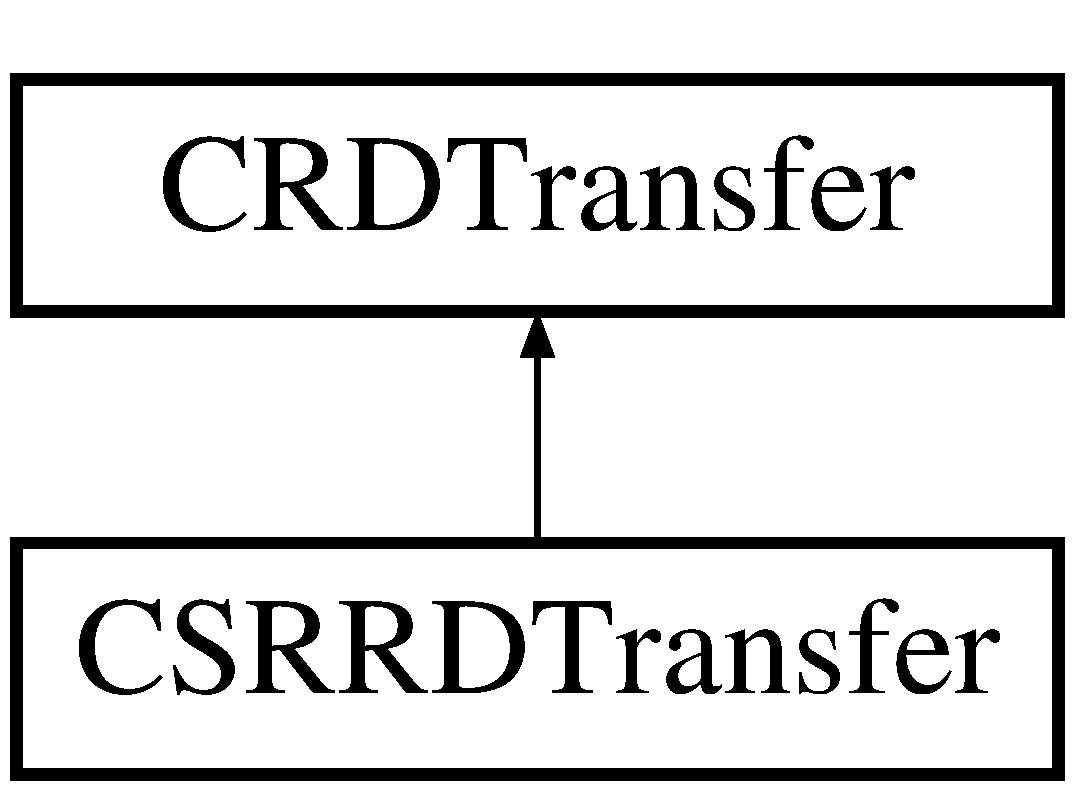
\includegraphics[height=2.000000cm]{class_c_s_r_r_d_transfer}
\end{center}
\end{figure}
\subsection*{Public 成员函数}
\begin{DoxyCompactItemize}
\item 
\hyperlink{class_c_s_r_r_d_transfer_a303368d342837dcc352b92ec9f3e887a}{C\+S\+R\+R\+D\+Transfer} ()
\item 
\hyperlink{class_c_s_r_r_d_transfer_a7bfdc212714609526efcd147a870259f}{$\sim$\+C\+S\+R\+R\+D\+Transfer} ()
\end{DoxyCompactItemize}
\subsection*{额外继承的成员函数}


\subsection{详细描述}


在文件 S\+R\+R\+D\+Transfer.\+h 第 3 行定义.



\subsection{构造及析构函数说明}
\mbox{\Hypertarget{class_c_s_r_r_d_transfer_a303368d342837dcc352b92ec9f3e887a}\label{class_c_s_r_r_d_transfer_a303368d342837dcc352b92ec9f3e887a}} 
\index{C\+S\+R\+R\+D\+Transfer@{C\+S\+R\+R\+D\+Transfer}!C\+S\+R\+R\+D\+Transfer@{C\+S\+R\+R\+D\+Transfer}}
\index{C\+S\+R\+R\+D\+Transfer@{C\+S\+R\+R\+D\+Transfer}!C\+S\+R\+R\+D\+Transfer@{C\+S\+R\+R\+D\+Transfer}}
\subsubsection{\texorpdfstring{C\+S\+R\+R\+D\+Transfer()}{CSRRDTransfer()}}
{\footnotesize\ttfamily C\+S\+R\+R\+D\+Transfer\+::\+C\+S\+R\+R\+D\+Transfer (\begin{DoxyParamCaption}{ }\end{DoxyParamCaption})}



在文件 S\+R\+R\+D\+Transfer.\+cpp 第 5 行定义.

\mbox{\Hypertarget{class_c_s_r_r_d_transfer_a7bfdc212714609526efcd147a870259f}\label{class_c_s_r_r_d_transfer_a7bfdc212714609526efcd147a870259f}} 
\index{C\+S\+R\+R\+D\+Transfer@{C\+S\+R\+R\+D\+Transfer}!````~C\+S\+R\+R\+D\+Transfer@{$\sim$\+C\+S\+R\+R\+D\+Transfer}}
\index{````~C\+S\+R\+R\+D\+Transfer@{$\sim$\+C\+S\+R\+R\+D\+Transfer}!C\+S\+R\+R\+D\+Transfer@{C\+S\+R\+R\+D\+Transfer}}
\subsubsection{\texorpdfstring{$\sim$\+C\+S\+R\+R\+D\+Transfer()}{~CSRRDTransfer()}}
{\footnotesize\ttfamily C\+S\+R\+R\+D\+Transfer\+::$\sim$\+C\+S\+R\+R\+D\+Transfer (\begin{DoxyParamCaption}{ }\end{DoxyParamCaption})}



在文件 S\+R\+R\+D\+Transfer.\+cpp 第 10 行定义.



该类的文档由以下文件生成\+:\begin{DoxyCompactItemize}
\item 
G\+:/华中科技大学/计卓1401/大三下/计算机网络/\+Layer\+Interface/\+T\+C\+P\+Layer/\hyperlink{_s_r_r_d_transfer_8h}{S\+R\+R\+D\+Transfer.\+h}\item 
G\+:/华中科技大学/计卓1401/大三下/计算机网络/\+Layer\+Interface/\+T\+C\+P\+Layer/\hyperlink{_s_r_r_d_transfer_8cpp}{S\+R\+R\+D\+Transfer.\+cpp}\end{DoxyCompactItemize}

\hypertarget{class_c_s_r_trans}{}\section{C\+S\+R\+Trans类 参考}
\label{class_c_s_r_trans}\index{C\+S\+R\+Trans@{C\+S\+R\+Trans}}


{\ttfamily \#include $<$S\+R\+Trans.\+h$>$}

类 C\+S\+R\+Trans 继承关系图\+:\begin{figure}[H]
\begin{center}
\leavevmode
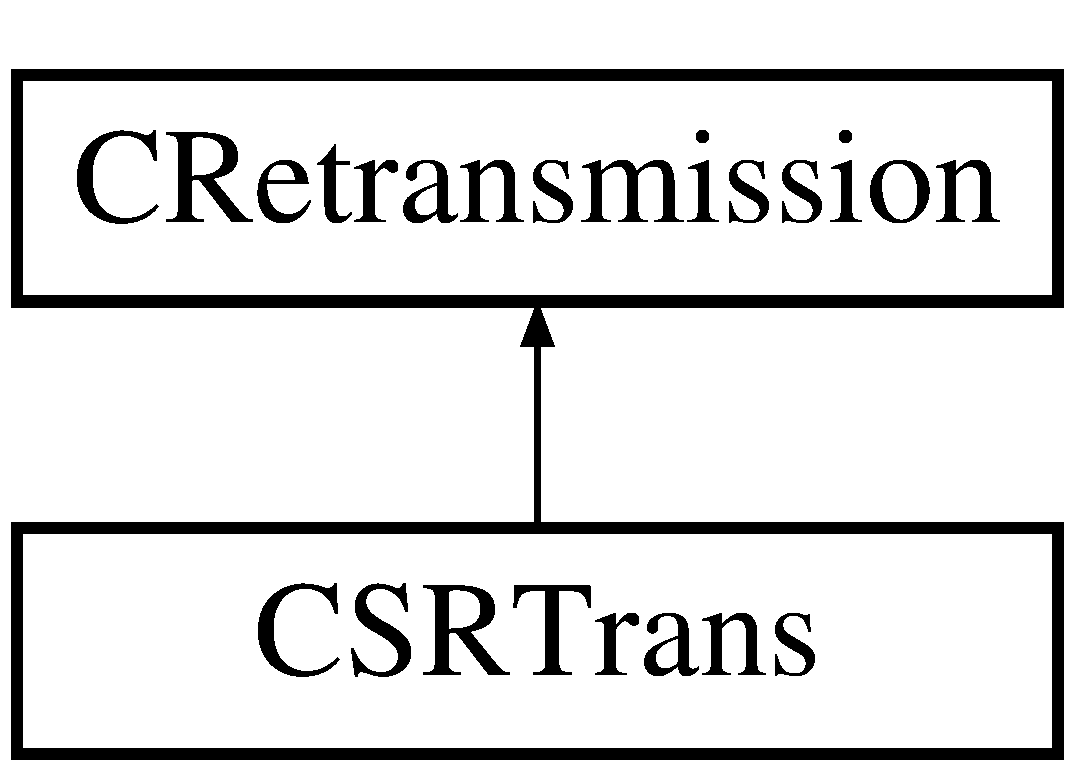
\includegraphics[height=2.000000cm]{class_c_s_r_trans}
\end{center}
\end{figure}
\subsection*{Public 成员函数}
\begin{DoxyCompactItemize}
\item 
\hyperlink{class_c_s_r_trans_ab13bd01789b3c571323d6848c80b3d07}{C\+S\+R\+Trans} ()
\item 
\hyperlink{class_c_s_r_trans_a6ead60de09d2a377c5527da55c7ec484}{$\sim$\+C\+S\+R\+Trans} ()
\end{DoxyCompactItemize}


\subsection{详细描述}


在文件 S\+R\+Trans.\+h 第 3 行定义.



\subsection{构造及析构函数说明}
\mbox{\Hypertarget{class_c_s_r_trans_ab13bd01789b3c571323d6848c80b3d07}\label{class_c_s_r_trans_ab13bd01789b3c571323d6848c80b3d07}} 
\index{C\+S\+R\+Trans@{C\+S\+R\+Trans}!C\+S\+R\+Trans@{C\+S\+R\+Trans}}
\index{C\+S\+R\+Trans@{C\+S\+R\+Trans}!C\+S\+R\+Trans@{C\+S\+R\+Trans}}
\subsubsection{\texorpdfstring{C\+S\+R\+Trans()}{CSRTrans()}}
{\footnotesize\ttfamily C\+S\+R\+Trans\+::\+C\+S\+R\+Trans (\begin{DoxyParamCaption}{ }\end{DoxyParamCaption})}



在文件 S\+R\+Trans.\+cpp 第 5 行定义.

\mbox{\Hypertarget{class_c_s_r_trans_a6ead60de09d2a377c5527da55c7ec484}\label{class_c_s_r_trans_a6ead60de09d2a377c5527da55c7ec484}} 
\index{C\+S\+R\+Trans@{C\+S\+R\+Trans}!````~C\+S\+R\+Trans@{$\sim$\+C\+S\+R\+Trans}}
\index{````~C\+S\+R\+Trans@{$\sim$\+C\+S\+R\+Trans}!C\+S\+R\+Trans@{C\+S\+R\+Trans}}
\subsubsection{\texorpdfstring{$\sim$\+C\+S\+R\+Trans()}{~CSRTrans()}}
{\footnotesize\ttfamily C\+S\+R\+Trans\+::$\sim$\+C\+S\+R\+Trans (\begin{DoxyParamCaption}{ }\end{DoxyParamCaption})}



在文件 S\+R\+Trans.\+cpp 第 10 行定义.



该类的文档由以下文件生成\+:\begin{DoxyCompactItemize}
\item 
G\+:/华中科技大学/计卓1401/大三下/计算机网络/\+Layer\+Interface/\+Transport\+Layer/\hyperlink{_s_r_trans_8h}{S\+R\+Trans.\+h}\item 
G\+:/华中科技大学/计卓1401/大三下/计算机网络/\+Layer\+Interface/\+Transport\+Layer/\hyperlink{_s_r_trans_8cpp}{S\+R\+Trans.\+cpp}\end{DoxyCompactItemize}

\hypertarget{class_c_t_c_p}{}\section{C\+T\+C\+P类 参考}
\label{class_c_t_c_p}\index{C\+T\+CP@{C\+T\+CP}}
类 C\+T\+CP 继承关系图\+:\begin{figure}[H]
\begin{center}
\leavevmode
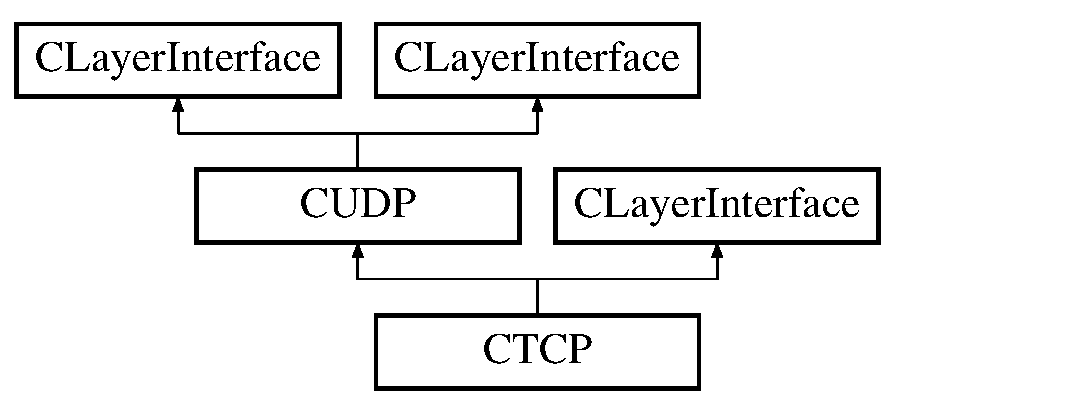
\includegraphics[height=3.000000cm]{class_c_t_c_p}
\end{center}
\end{figure}
\subsection*{Public 成员函数}
\begin{DoxyCompactItemize}
\item 
\mbox{\Hypertarget{class_c_t_c_p_a7dee32e3cae74e448df0b4d09fea3d43}\label{class_c_t_c_p_a7dee32e3cae74e448df0b4d09fea3d43}} 
{\bfseries C\+T\+CP} (\hyperlink{class_msg_list}{Msg\+List} \&send\+Buf, \hyperlink{class_msg_list}{Msg\+List} \&rcv\+Buf)
\item 
\mbox{\Hypertarget{class_c_t_c_p_a2437e907d98e436a994c6395f59bf851}\label{class_c_t_c_p_a2437e907d98e436a994c6395f59bf851}} 
bool {\bfseries connect} (char $\ast$ip, int port)
\item 
\mbox{\Hypertarget{class_c_t_c_p_ab1b3f5ede8f15181ecd3355763e75892}\label{class_c_t_c_p_ab1b3f5ede8f15181ecd3355763e75892}} 
bool {\bfseries close} (char $\ast$ip, int port)
\item 
\mbox{\Hypertarget{class_c_t_c_p_a4552b74145e832f32c1cb45a9fa2a5e9}\label{class_c_t_c_p_a4552b74145e832f32c1cb45a9fa2a5e9}} 
bool {\bfseries send\+Data} (\hyperlink{class_datagram}{Datagram} data)
\item 
\mbox{\Hypertarget{class_c_t_c_p_aed8fdd632e22efee66dbbb95e951b5c2}\label{class_c_t_c_p_aed8fdd632e22efee66dbbb95e951b5c2}} 
bool {\bfseries recv\+Data} (\hyperlink{class_datagram}{Datagram} data)
\item 
\mbox{\Hypertarget{class_c_t_c_p_a7dee32e3cae74e448df0b4d09fea3d43}\label{class_c_t_c_p_a7dee32e3cae74e448df0b4d09fea3d43}} 
{\bfseries C\+T\+CP} (\hyperlink{class_msg_list}{Msg\+List} \&send\+Buf, \hyperlink{class_msg_list}{Msg\+List} \&rcv\+Buf)
\item 
\mbox{\Hypertarget{class_c_t_c_p_a0af93bbde343608a81a4772c38bbdfa6}\label{class_c_t_c_p_a0af93bbde343608a81a4772c38bbdfa6}} 
bool {\bfseries connect} ()
\item 
\mbox{\Hypertarget{class_c_t_c_p_a382a93d27e10a726d0464402e22517b8}\label{class_c_t_c_p_a382a93d27e10a726d0464402e22517b8}} 
bool {\bfseries disconnect} ()
\end{DoxyCompactItemize}
\subsection*{Protected 成员函数}
\begin{DoxyCompactItemize}
\item 
\mbox{\Hypertarget{class_c_t_c_p_a0c68800a3b6317cbe74aa2cb28ea3d9c}\label{class_c_t_c_p_a0c68800a3b6317cbe74aa2cb28ea3d9c}} 
void {\bfseries add\+Head} ()
\item 
\mbox{\Hypertarget{class_c_t_c_p_a0c68800a3b6317cbe74aa2cb28ea3d9c}\label{class_c_t_c_p_a0c68800a3b6317cbe74aa2cb28ea3d9c}} 
void {\bfseries add\+Head} ()
\end{DoxyCompactItemize}
\subsection*{额外继承的成员函数}


该类的文档由以下文件生成\+:\begin{DoxyCompactItemize}
\item 
G\+:/华中科技大学/计卓1401/大三下/计算机网络/\+Layer\+Interface/\+T\+C\+P\+Layer/T\+C\+P\+Layer.\+h\item 
G\+:/华中科技大学/计卓1401/大三下/计算机网络/\+Layer\+Interface/\+Transport\+Layer/T\+C\+P.\+h\item 
G\+:/华中科技大学/计卓1401/大三下/计算机网络/\+Layer\+Interface/\+T\+C\+P\+Layer/T\+C\+P\+Layer.\+cpp\item 
G\+:/华中科技大学/计卓1401/大三下/计算机网络/\+Layer\+Interface/\+Transport\+Layer/T\+C\+P.\+cpp\end{DoxyCompactItemize}

\hypertarget{class_c_t_c_p_connect}{}\section{C\+T\+C\+P\+Connect类 参考}
\label{class_c_t_c_p_connect}\index{C\+T\+C\+P\+Connect@{C\+T\+C\+P\+Connect}}


{\ttfamily \#include $<$T\+C\+P\+Connect.\+h$>$}

\subsection*{Public 成员函数}
\begin{DoxyCompactItemize}
\item 
\hyperlink{class_c_t_c_p_connect_aeb3034135b26b22b54cd3f44691f2744}{C\+T\+C\+P\+Connect} ()
\item 
\hyperlink{class_c_t_c_p_connect_a9f5247e1a88170a943ba0b5c4b07b26c}{$\sim$\+C\+T\+C\+P\+Connect} ()
\end{DoxyCompactItemize}
\subsection*{Public 属性}
\begin{DoxyCompactItemize}
\item 
\hyperlink{class_c_layer_interface}{C\+Layer\+Interface} $\ast$ \hyperlink{class_c_t_c_p_connect_a0418f1607ff29af6941d080cf5896df7}{m\+\_\+p\+C\+T\+CP}
\end{DoxyCompactItemize}


\subsection{详细描述}


在文件 T\+C\+P\+Connect.\+h 第 3 行定义.



\subsection{构造及析构函数说明}
\mbox{\Hypertarget{class_c_t_c_p_connect_aeb3034135b26b22b54cd3f44691f2744}\label{class_c_t_c_p_connect_aeb3034135b26b22b54cd3f44691f2744}} 
\index{C\+T\+C\+P\+Connect@{C\+T\+C\+P\+Connect}!C\+T\+C\+P\+Connect@{C\+T\+C\+P\+Connect}}
\index{C\+T\+C\+P\+Connect@{C\+T\+C\+P\+Connect}!C\+T\+C\+P\+Connect@{C\+T\+C\+P\+Connect}}
\subsubsection{\texorpdfstring{C\+T\+C\+P\+Connect()}{CTCPConnect()}}
{\footnotesize\ttfamily C\+T\+C\+P\+Connect\+::\+C\+T\+C\+P\+Connect (\begin{DoxyParamCaption}{ }\end{DoxyParamCaption})}



在文件 T\+C\+P\+Connect.\+cpp 第 5 行定义.

\mbox{\Hypertarget{class_c_t_c_p_connect_a9f5247e1a88170a943ba0b5c4b07b26c}\label{class_c_t_c_p_connect_a9f5247e1a88170a943ba0b5c4b07b26c}} 
\index{C\+T\+C\+P\+Connect@{C\+T\+C\+P\+Connect}!````~C\+T\+C\+P\+Connect@{$\sim$\+C\+T\+C\+P\+Connect}}
\index{````~C\+T\+C\+P\+Connect@{$\sim$\+C\+T\+C\+P\+Connect}!C\+T\+C\+P\+Connect@{C\+T\+C\+P\+Connect}}
\subsubsection{\texorpdfstring{$\sim$\+C\+T\+C\+P\+Connect()}{~CTCPConnect()}}
{\footnotesize\ttfamily C\+T\+C\+P\+Connect\+::$\sim$\+C\+T\+C\+P\+Connect (\begin{DoxyParamCaption}{ }\end{DoxyParamCaption})}



在文件 T\+C\+P\+Connect.\+cpp 第 10 行定义.



\subsection{类成员变量说明}
\mbox{\Hypertarget{class_c_t_c_p_connect_a0418f1607ff29af6941d080cf5896df7}\label{class_c_t_c_p_connect_a0418f1607ff29af6941d080cf5896df7}} 
\index{C\+T\+C\+P\+Connect@{C\+T\+C\+P\+Connect}!m\+\_\+p\+C\+T\+CP@{m\+\_\+p\+C\+T\+CP}}
\index{m\+\_\+p\+C\+T\+CP@{m\+\_\+p\+C\+T\+CP}!C\+T\+C\+P\+Connect@{C\+T\+C\+P\+Connect}}
\subsubsection{\texorpdfstring{m\+\_\+p\+C\+T\+CP}{m\_pCTCP}}
{\footnotesize\ttfamily \hyperlink{class_c_layer_interface}{C\+Layer\+Interface}$\ast$ C\+T\+C\+P\+Connect\+::m\+\_\+p\+C\+T\+CP}



在文件 T\+C\+P\+Connect.\+h 第 10 行定义.



该类的文档由以下文件生成\+:\begin{DoxyCompactItemize}
\item 
G\+:/华中科技大学/计卓1401/大三下/计算机网络/\+Layer\+Interface/\+T\+C\+P\+Layer/\hyperlink{_t_c_p_connect_8h}{T\+C\+P\+Connect.\+h}\item 
G\+:/华中科技大学/计卓1401/大三下/计算机网络/\+Layer\+Interface/\+T\+C\+P\+Layer/\hyperlink{_t_c_p_connect_8cpp}{T\+C\+P\+Connect.\+cpp}\end{DoxyCompactItemize}

\hypertarget{class_c_tranmission_ctrl}{}\section{C\+Tranmission\+Ctrl类 参考}
\label{class_c_tranmission_ctrl}\index{C\+Tranmission\+Ctrl@{C\+Tranmission\+Ctrl}}
\subsection*{Public 成员函数}
\begin{DoxyCompactItemize}
\item 
\mbox{\Hypertarget{class_c_tranmission_ctrl_a788cf64847e7345d6f82080a539431eb}\label{class_c_tranmission_ctrl_a788cf64847e7345d6f82080a539431eb}} 
void {\bfseries set\+Window} ()
\end{DoxyCompactItemize}
\subsection*{Public 属性}
\begin{DoxyCompactItemize}
\item 
\mbox{\Hypertarget{class_c_tranmission_ctrl_a78277227cfa57679025eaffe98b3807c}\label{class_c_tranmission_ctrl_a78277227cfa57679025eaffe98b3807c}} 
\hyperlink{class_c_window}{C\+Window} $\ast$ {\bfseries window}
\end{DoxyCompactItemize}


该类的文档由以下文件生成\+:\begin{DoxyCompactItemize}
\item 
G\+:/华中科技大学/计卓1401/大三下/计算机网络/\+Layer\+Interface/\+Transport\+Layer/Tranmission\+Ctrl.\+h\item 
G\+:/华中科技大学/计卓1401/大三下/计算机网络/\+Layer\+Interface/\+Transport\+Layer/Tranmission\+Ctrl.\+cpp\end{DoxyCompactItemize}

\hypertarget{class_c_transport_layer}{}\section{C\+Transport\+Layer类 参考}
\label{class_c_transport_layer}\index{C\+Transport\+Layer@{C\+Transport\+Layer}}
类 C\+Transport\+Layer 继承关系图\+:\begin{figure}[H]
\begin{center}
\leavevmode
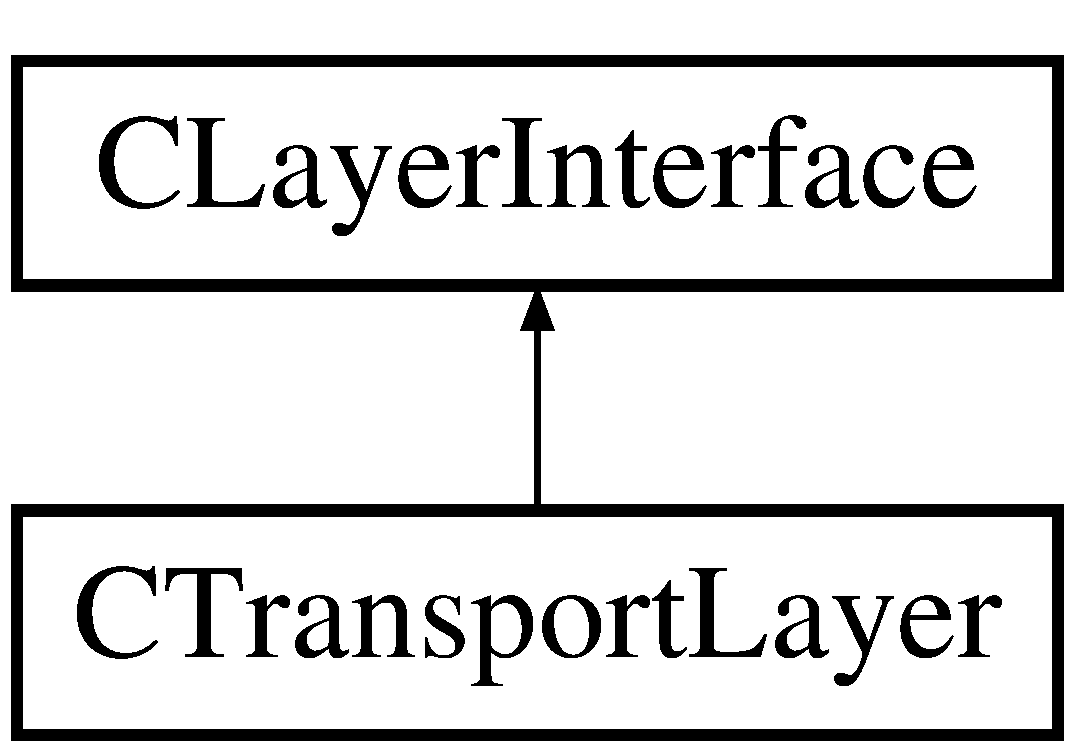
\includegraphics[height=2.000000cm]{class_c_transport_layer}
\end{center}
\end{figure}
\subsection*{Public 成员函数}
\begin{DoxyCompactItemize}
\item 
\mbox{\Hypertarget{class_c_transport_layer_ac81e9405db824a73a6092ed0b05a217b}\label{class_c_transport_layer_ac81e9405db824a73a6092ed0b05a217b}} 
bool {\bfseries init} ()
\item 
\mbox{\Hypertarget{class_c_transport_layer_a60d1d41f33c5662eb9c1bbd1c8aa4dc3}\label{class_c_transport_layer_a60d1d41f33c5662eb9c1bbd1c8aa4dc3}} 
void {\bfseries run} ()
\item 
\mbox{\Hypertarget{class_c_transport_layer_a5755c5d7f4158bb08303b98042b24ca1}\label{class_c_transport_layer_a5755c5d7f4158bb08303b98042b24ca1}} 
void {\bfseries send\+Transfer} ()
\item 
\mbox{\Hypertarget{class_c_transport_layer_ad30133ccd6047d127d5a9feec593877d}\label{class_c_transport_layer_ad30133ccd6047d127d5a9feec593877d}} 
void {\bfseries recv\+Transfer} ()
\item 
\mbox{\Hypertarget{class_c_transport_layer_a9396850eb026ff070c06bfc25dd4979c}\label{class_c_transport_layer_a9396850eb026ff070c06bfc25dd4979c}} 
\hyperlink{class_datagram}{Datagram} {\bfseries get\+Data} (int lable)
\item 
\mbox{\Hypertarget{class_c_transport_layer_a6ee36bbbfab91014087ed88923129372}\label{class_c_transport_layer_a6ee36bbbfab91014087ed88923129372}} 
\hyperlink{class_datagram}{Datagram} {\bfseries get\+Datagram} ()
\item 
\mbox{\Hypertarget{class_c_transport_layer_a18cba0784dba2a15f051be2c1163c278}\label{class_c_transport_layer_a18cba0784dba2a15f051be2c1163c278}} 
bool {\bfseries is\+Recv\+Buf\+Empty} ()
\item 
\mbox{\Hypertarget{class_c_transport_layer_aace17995c3cff74c756ecdb2a2e8cf43}\label{class_c_transport_layer_aace17995c3cff74c756ecdb2a2e8cf43}} 
bool {\bfseries is\+Buffer\+Ready} (int lable)
\item 
\mbox{\Hypertarget{class_c_transport_layer_a5830c0965a4a9501ffb33ae8d2acb58b}\label{class_c_transport_layer_a5830c0965a4a9501ffb33ae8d2acb58b}} 
int {\bfseries connect} ()
\item 
\mbox{\Hypertarget{class_c_transport_layer_a603dcfda4b1ef7dfb58c922cd8fd59bb}\label{class_c_transport_layer_a603dcfda4b1ef7dfb58c922cd8fd59bb}} 
int {\bfseries disconnect} ()
\item 
\mbox{\Hypertarget{class_c_transport_layer_abce8f3ca4b9c4d5c957b0f7b6746f289}\label{class_c_transport_layer_abce8f3ca4b9c4d5c957b0f7b6746f289}} 
void {\bfseries multiplex} ()
\item 
\mbox{\Hypertarget{class_c_transport_layer_a3cbec0cdcdcf91df91ae7c708d8a414c}\label{class_c_transport_layer_a3cbec0cdcdcf91df91ae7c708d8a414c}} 
void {\bfseries demultiplex} ()
\item 
\mbox{\Hypertarget{class_c_transport_layer_aa5d4c185f3a0f9c968d51caf46f7332e}\label{class_c_transport_layer_aa5d4c185f3a0f9c968d51caf46f7332e}} 
void {\bfseries multiplex} (\hyperlink{class_datagram}{Datagram} data)
\item 
\mbox{\Hypertarget{class_c_transport_layer_a316dd2a423992b04d77d42198c4e421c}\label{class_c_transport_layer_a316dd2a423992b04d77d42198c4e421c}} 
void {\bfseries demultiplex} (\hyperlink{class_datagram}{Datagram} data)
\end{DoxyCompactItemize}
\subsection*{额外继承的成员函数}


该类的文档由以下文件生成\+:\begin{DoxyCompactItemize}
\item 
G\+:/华中科技大学/计卓1401/大三下/计算机网络/\+Layer\+Interface/\+Transport\+Layer/Transport\+Layer.\+h\item 
G\+:/华中科技大学/计卓1401/大三下/计算机网络/\+Layer\+Interface/\+Transport\+Layer/Transport\+Layer.\+cpp\end{DoxyCompactItemize}

\hypertarget{class_c_trans_table}{}\section{C\+Trans\+Table类 参考}
\label{class_c_trans_table}\index{C\+Trans\+Table@{C\+Trans\+Table}}


{\ttfamily \#include $<$N\+A\+T\+Proto.\+h$>$}



\subsection{详细描述}


在文件 N\+A\+T\+Proto.\+h 第 6 行定义.



该类的文档由以下文件生成\+:\begin{DoxyCompactItemize}
\item 
G\+:/华中科技大学/计卓1401/大三下/计算机网络/\+Layer\+Interface/\+I\+P\+Layer/\hyperlink{_n_a_t_proto_8h}{N\+A\+T\+Proto.\+h}\end{DoxyCompactItemize}

\hypertarget{class_c_u_d_p}{}\section{C\+U\+D\+P类 参考}
\label{class_c_u_d_p}\index{C\+U\+DP@{C\+U\+DP}}


{\ttfamily \#include $<$U\+D\+P.\+h$>$}

类 C\+U\+DP 继承关系图\+:\begin{figure}[H]
\begin{center}
\leavevmode
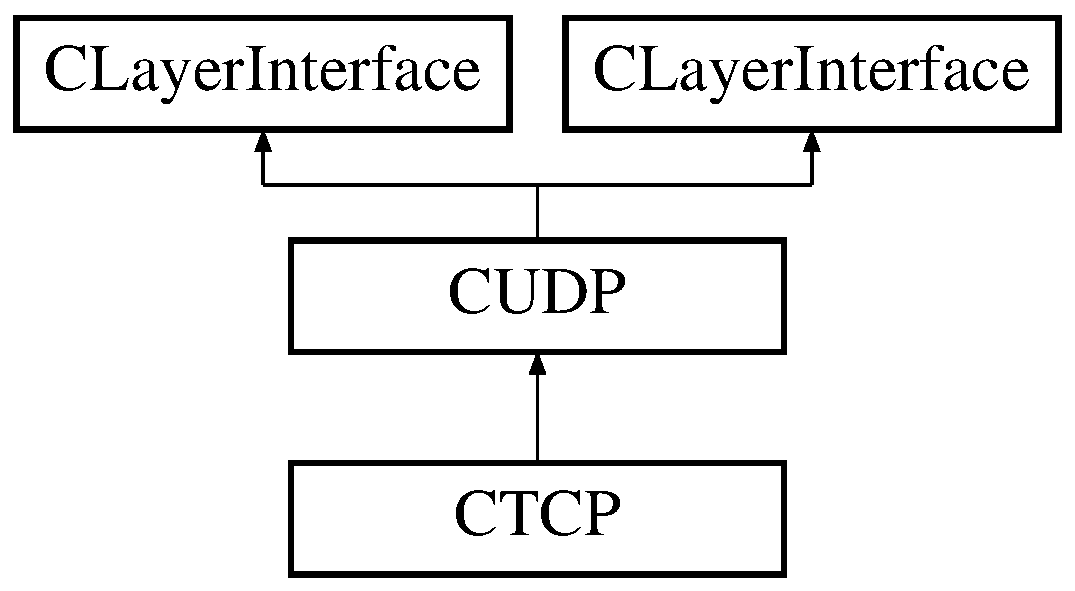
\includegraphics[height=3.000000cm]{class_c_u_d_p}
\end{center}
\end{figure}
\subsection*{Public 成员函数}
\begin{DoxyCompactItemize}
\item 
\hyperlink{class_c_u_d_p_a2eed7862494fbdc41005e5f536d2f74f}{C\+U\+DP} (\hyperlink{class_msg_list}{Msg\+List} \&send\+Buf, \hyperlink{class_msg_list}{Msg\+List} \&rcv\+Buf)
\item 
\hyperlink{class_c_u_d_p_aa5e4b24a48885c739893d60ffb10672f}{$\sim$\+C\+U\+DP} ()
\item 
bool \hyperlink{class_c_u_d_p_af595428bc531576d9859a9e0b84d03d9}{is\+Buffer\+Ready} (int lable)
\item 
bool \hyperlink{class_c_u_d_p_a1f6e555ad4997b283e68ebfa7dc0d263}{send\+Data} (\hyperlink{class_datagram}{Datagram} datagram)
\item 
\hyperlink{class_datagram}{Datagram} \hyperlink{class_c_u_d_p_aa71e49c760769b55dc2251b244eb00ff}{get\+Data} (int lable)
\item 
\hyperlink{class_c_u_d_p_a2eed7862494fbdc41005e5f536d2f74f}{C\+U\+DP} (\hyperlink{class_msg_list}{Msg\+List} \&send\+Buf, \hyperlink{class_msg_list}{Msg\+List} \&rcv\+Buf)
\item 
bool \hyperlink{class_c_u_d_p_a08619144028e752736166988369598c4}{init} ()
\item 
\hyperlink{class_c_u_d_p_aa5e4b24a48885c739893d60ffb10672f}{$\sim$\+C\+U\+DP} ()
\item 
void \hyperlink{class_c_u_d_p_a32181d9f38654f9480193af29fc221eb}{add\+Client} (\hyperlink{class_msg_list}{Msg\+List} send\+Buf, \hyperlink{class_msg_list}{Msg\+List} rcv\+Buf)
\end{DoxyCompactItemize}
\subsection*{Public 属性}
\begin{DoxyCompactItemize}
\item 
\hyperlink{class_c_transport_layer}{C\+Transport\+Layer} $\ast$ \hyperlink{class_c_u_d_p_a4c0a9bc6c679d857a3461a3a71ba8abd}{outer\+Layer}
\end{DoxyCompactItemize}
\subsection*{Protected 成员函数}
\begin{DoxyCompactItemize}
\item 
void \hyperlink{class_c_u_d_p_a445c3b7fe1b58e8b278115649ad25c3f}{add\+Head} ()
\item 
void \hyperlink{class_c_u_d_p_a445c3b7fe1b58e8b278115649ad25c3f}{add\+Head} ()
\end{DoxyCompactItemize}
\subsection*{Protected 属性}
\begin{DoxyCompactItemize}
\item 
std\+::vector$<$ \hyperlink{class_msg_list}{Msg\+List} $\ast$ $>$ \hyperlink{class_c_u_d_p_adc6c3097ec9ab885987b058ef3b1e26f}{m\+\_\+\+Msg\+List\+Send\+Que}
\item 
int \hyperlink{class_c_u_d_p_acf38f880b4ccfbff285aeaff75a931a4}{m\+\_\+i\+Send\+Que\+Tail}
\item 
std\+::vector$<$ \hyperlink{class_msg_list}{Msg\+List} $\ast$ $>$ \hyperlink{class_c_u_d_p_ae04cfd9b77ae1d4f96d83e890a1203f3}{m\+\_\+\+Msg\+List\+Recv\+Que}
\item 
int \hyperlink{class_c_u_d_p_ae90f37aa5c56ecf05cf6e4daacd90bba}{m\+\_\+i\+Recv\+Que\+Tail}
\end{DoxyCompactItemize}
\subsection*{额外继承的成员函数}


\subsection{详细描述}


在文件 U\+D\+P.\+h 第 6 行定义.



\subsection{构造及析构函数说明}
\mbox{\Hypertarget{class_c_u_d_p_a2eed7862494fbdc41005e5f536d2f74f}\label{class_c_u_d_p_a2eed7862494fbdc41005e5f536d2f74f}} 
\index{C\+U\+DP@{C\+U\+DP}!C\+U\+DP@{C\+U\+DP}}
\index{C\+U\+DP@{C\+U\+DP}!C\+U\+DP@{C\+U\+DP}}
\subsubsection{\texorpdfstring{C\+U\+D\+P()}{CUDP()}\hspace{0.1cm}{\footnotesize\ttfamily [1/2]}}
{\footnotesize\ttfamily C\+U\+D\+P\+::\+C\+U\+DP (\begin{DoxyParamCaption}\item[{\hyperlink{class_msg_list}{Msg\+List} \&}]{send\+Buf,  }\item[{\hyperlink{class_msg_list}{Msg\+List} \&}]{rcv\+Buf }\end{DoxyParamCaption})}



在文件 U\+D\+P.\+cpp 第 5 行定义.

\mbox{\Hypertarget{class_c_u_d_p_aa5e4b24a48885c739893d60ffb10672f}\label{class_c_u_d_p_aa5e4b24a48885c739893d60ffb10672f}} 
\index{C\+U\+DP@{C\+U\+DP}!````~C\+U\+DP@{$\sim$\+C\+U\+DP}}
\index{````~C\+U\+DP@{$\sim$\+C\+U\+DP}!C\+U\+DP@{C\+U\+DP}}
\subsubsection{\texorpdfstring{$\sim$\+C\+U\+D\+P()}{~CUDP()}\hspace{0.1cm}{\footnotesize\ttfamily [1/2]}}
{\footnotesize\ttfamily C\+U\+D\+P\+::$\sim$\+C\+U\+DP (\begin{DoxyParamCaption}{ }\end{DoxyParamCaption})}



在文件 U\+D\+P.\+cpp 第 16 行定义.

\mbox{\Hypertarget{class_c_u_d_p_a2eed7862494fbdc41005e5f536d2f74f}\label{class_c_u_d_p_a2eed7862494fbdc41005e5f536d2f74f}} 
\index{C\+U\+DP@{C\+U\+DP}!C\+U\+DP@{C\+U\+DP}}
\index{C\+U\+DP@{C\+U\+DP}!C\+U\+DP@{C\+U\+DP}}
\subsubsection{\texorpdfstring{C\+U\+D\+P()}{CUDP()}\hspace{0.1cm}{\footnotesize\ttfamily [2/2]}}
{\footnotesize\ttfamily C\+U\+D\+P\+::\+C\+U\+DP (\begin{DoxyParamCaption}\item[{\hyperlink{class_msg_list}{Msg\+List} \&}]{send\+Buf,  }\item[{\hyperlink{class_msg_list}{Msg\+List} \&}]{rcv\+Buf }\end{DoxyParamCaption})}

\mbox{\Hypertarget{class_c_u_d_p_aa5e4b24a48885c739893d60ffb10672f}\label{class_c_u_d_p_aa5e4b24a48885c739893d60ffb10672f}} 
\index{C\+U\+DP@{C\+U\+DP}!````~C\+U\+DP@{$\sim$\+C\+U\+DP}}
\index{````~C\+U\+DP@{$\sim$\+C\+U\+DP}!C\+U\+DP@{C\+U\+DP}}
\subsubsection{\texorpdfstring{$\sim$\+C\+U\+D\+P()}{~CUDP()}\hspace{0.1cm}{\footnotesize\ttfamily [2/2]}}
{\footnotesize\ttfamily C\+U\+D\+P\+::$\sim$\+C\+U\+DP (\begin{DoxyParamCaption}{ }\end{DoxyParamCaption})}



\subsection{成员函数说明}
\mbox{\Hypertarget{class_c_u_d_p_a32181d9f38654f9480193af29fc221eb}\label{class_c_u_d_p_a32181d9f38654f9480193af29fc221eb}} 
\index{C\+U\+DP@{C\+U\+DP}!add\+Client@{add\+Client}}
\index{add\+Client@{add\+Client}!C\+U\+DP@{C\+U\+DP}}
\subsubsection{\texorpdfstring{add\+Client()}{addClient()}}
{\footnotesize\ttfamily void C\+U\+D\+P\+::add\+Client (\begin{DoxyParamCaption}\item[{\hyperlink{class_msg_list}{Msg\+List}}]{send\+Buf,  }\item[{\hyperlink{class_msg_list}{Msg\+List}}]{rcv\+Buf }\end{DoxyParamCaption})}



在文件 C\+U\+D\+P.\+cpp 第 21 行定义.

\mbox{\Hypertarget{class_c_u_d_p_a445c3b7fe1b58e8b278115649ad25c3f}\label{class_c_u_d_p_a445c3b7fe1b58e8b278115649ad25c3f}} 
\index{C\+U\+DP@{C\+U\+DP}!add\+Head@{add\+Head}}
\index{add\+Head@{add\+Head}!C\+U\+DP@{C\+U\+DP}}
\subsubsection{\texorpdfstring{add\+Head()}{addHead()}\hspace{0.1cm}{\footnotesize\ttfamily [1/2]}}
{\footnotesize\ttfamily void C\+U\+D\+P\+::add\+Head (\begin{DoxyParamCaption}{ }\end{DoxyParamCaption})\hspace{0.3cm}{\ttfamily [protected]}, {\ttfamily [virtual]}}



重载 \hyperlink{class_c_layer_interface_ac38c51660960657ac42e37a19ea062b4}{C\+Layer\+Interface} .



在文件 U\+D\+P.\+cpp 第 21 行定义.

\mbox{\Hypertarget{class_c_u_d_p_a445c3b7fe1b58e8b278115649ad25c3f}\label{class_c_u_d_p_a445c3b7fe1b58e8b278115649ad25c3f}} 
\index{C\+U\+DP@{C\+U\+DP}!add\+Head@{add\+Head}}
\index{add\+Head@{add\+Head}!C\+U\+DP@{C\+U\+DP}}
\subsubsection{\texorpdfstring{add\+Head()}{addHead()}\hspace{0.1cm}{\footnotesize\ttfamily [2/2]}}
{\footnotesize\ttfamily void C\+U\+D\+P\+::add\+Head (\begin{DoxyParamCaption}{ }\end{DoxyParamCaption})\hspace{0.3cm}{\ttfamily [protected]}, {\ttfamily [virtual]}}



重载 \hyperlink{class_c_layer_interface_ac38c51660960657ac42e37a19ea062b4}{C\+Layer\+Interface} .

\mbox{\Hypertarget{class_c_u_d_p_aa71e49c760769b55dc2251b244eb00ff}\label{class_c_u_d_p_aa71e49c760769b55dc2251b244eb00ff}} 
\index{C\+U\+DP@{C\+U\+DP}!get\+Data@{get\+Data}}
\index{get\+Data@{get\+Data}!C\+U\+DP@{C\+U\+DP}}
\subsubsection{\texorpdfstring{get\+Data()}{getData()}}
{\footnotesize\ttfamily \hyperlink{class_datagram}{Datagram} C\+U\+D\+P\+::get\+Data (\begin{DoxyParamCaption}\item[{int}]{lable }\end{DoxyParamCaption})\hspace{0.3cm}{\ttfamily [virtual]}}

get data from the buffer 

重载 \hyperlink{class_c_layer_interface_a804d604d3e0032e676d02fd5d369607e}{C\+Layer\+Interface} .



在文件 U\+D\+P.\+cpp 第 35 行定义.

\mbox{\Hypertarget{class_c_u_d_p_a08619144028e752736166988369598c4}\label{class_c_u_d_p_a08619144028e752736166988369598c4}} 
\index{C\+U\+DP@{C\+U\+DP}!init@{init}}
\index{init@{init}!C\+U\+DP@{C\+U\+DP}}
\subsubsection{\texorpdfstring{init()}{init()}}
{\footnotesize\ttfamily bool C\+U\+D\+P\+::init (\begin{DoxyParamCaption}{ }\end{DoxyParamCaption})}



在文件 C\+U\+D\+P.\+cpp 第 30 行定义.

\mbox{\Hypertarget{class_c_u_d_p_af595428bc531576d9859a9e0b84d03d9}\label{class_c_u_d_p_af595428bc531576d9859a9e0b84d03d9}} 
\index{C\+U\+DP@{C\+U\+DP}!is\+Buffer\+Ready@{is\+Buffer\+Ready}}
\index{is\+Buffer\+Ready@{is\+Buffer\+Ready}!C\+U\+DP@{C\+U\+DP}}
\subsubsection{\texorpdfstring{is\+Buffer\+Ready()}{isBufferReady()}}
{\footnotesize\ttfamily bool C\+U\+D\+P\+::is\+Buffer\+Ready (\begin{DoxyParamCaption}\item[{int}]{lable }\end{DoxyParamCaption})\hspace{0.3cm}{\ttfamily [virtual]}}

check if the buffer can be used 

重载 \hyperlink{class_c_layer_interface_a4979d7b5740c06be048e4b0f1195c8fc}{C\+Layer\+Interface} .



在文件 U\+D\+P.\+cpp 第 46 行定义.

\mbox{\Hypertarget{class_c_u_d_p_a1f6e555ad4997b283e68ebfa7dc0d263}\label{class_c_u_d_p_a1f6e555ad4997b283e68ebfa7dc0d263}} 
\index{C\+U\+DP@{C\+U\+DP}!send\+Data@{send\+Data}}
\index{send\+Data@{send\+Data}!C\+U\+DP@{C\+U\+DP}}
\subsubsection{\texorpdfstring{send\+Data()}{sendData()}}
{\footnotesize\ttfamily bool C\+U\+D\+P\+::send\+Data (\begin{DoxyParamCaption}\item[{\hyperlink{class_datagram}{Datagram}}]{data }\end{DoxyParamCaption})\hspace{0.3cm}{\ttfamily [virtual]}}

insert the data into buffer 

重载 \hyperlink{class_c_layer_interface_ae5115cf6ee0e76247dac067cc797a06b}{C\+Layer\+Interface} .



在文件 U\+D\+P.\+cpp 第 30 行定义.



\subsection{类成员变量说明}
\mbox{\Hypertarget{class_c_u_d_p_ae90f37aa5c56ecf05cf6e4daacd90bba}\label{class_c_u_d_p_ae90f37aa5c56ecf05cf6e4daacd90bba}} 
\index{C\+U\+DP@{C\+U\+DP}!m\+\_\+i\+Recv\+Que\+Tail@{m\+\_\+i\+Recv\+Que\+Tail}}
\index{m\+\_\+i\+Recv\+Que\+Tail@{m\+\_\+i\+Recv\+Que\+Tail}!C\+U\+DP@{C\+U\+DP}}
\subsubsection{\texorpdfstring{m\+\_\+i\+Recv\+Que\+Tail}{m\_iRecvQueTail}}
{\footnotesize\ttfamily int C\+U\+D\+P\+::m\+\_\+i\+Recv\+Que\+Tail\hspace{0.3cm}{\ttfamily [protected]}}



在文件 C\+U\+D\+P.\+h 第 24 行定义.

\mbox{\Hypertarget{class_c_u_d_p_acf38f880b4ccfbff285aeaff75a931a4}\label{class_c_u_d_p_acf38f880b4ccfbff285aeaff75a931a4}} 
\index{C\+U\+DP@{C\+U\+DP}!m\+\_\+i\+Send\+Que\+Tail@{m\+\_\+i\+Send\+Que\+Tail}}
\index{m\+\_\+i\+Send\+Que\+Tail@{m\+\_\+i\+Send\+Que\+Tail}!C\+U\+DP@{C\+U\+DP}}
\subsubsection{\texorpdfstring{m\+\_\+i\+Send\+Que\+Tail}{m\_iSendQueTail}}
{\footnotesize\ttfamily int C\+U\+D\+P\+::m\+\_\+i\+Send\+Que\+Tail\hspace{0.3cm}{\ttfamily [protected]}}



在文件 C\+U\+D\+P.\+h 第 22 行定义.

\mbox{\Hypertarget{class_c_u_d_p_ae04cfd9b77ae1d4f96d83e890a1203f3}\label{class_c_u_d_p_ae04cfd9b77ae1d4f96d83e890a1203f3}} 
\index{C\+U\+DP@{C\+U\+DP}!m\+\_\+\+Msg\+List\+Recv\+Que@{m\+\_\+\+Msg\+List\+Recv\+Que}}
\index{m\+\_\+\+Msg\+List\+Recv\+Que@{m\+\_\+\+Msg\+List\+Recv\+Que}!C\+U\+DP@{C\+U\+DP}}
\subsubsection{\texorpdfstring{m\+\_\+\+Msg\+List\+Recv\+Que}{m\_MsgListRecvQue}}
{\footnotesize\ttfamily std\+::vector$<$\hyperlink{class_msg_list}{Msg\+List}$\ast$$>$ C\+U\+D\+P\+::m\+\_\+\+Msg\+List\+Recv\+Que\hspace{0.3cm}{\ttfamily [protected]}}



在文件 C\+U\+D\+P.\+h 第 23 行定义.

\mbox{\Hypertarget{class_c_u_d_p_adc6c3097ec9ab885987b058ef3b1e26f}\label{class_c_u_d_p_adc6c3097ec9ab885987b058ef3b1e26f}} 
\index{C\+U\+DP@{C\+U\+DP}!m\+\_\+\+Msg\+List\+Send\+Que@{m\+\_\+\+Msg\+List\+Send\+Que}}
\index{m\+\_\+\+Msg\+List\+Send\+Que@{m\+\_\+\+Msg\+List\+Send\+Que}!C\+U\+DP@{C\+U\+DP}}
\subsubsection{\texorpdfstring{m\+\_\+\+Msg\+List\+Send\+Que}{m\_MsgListSendQue}}
{\footnotesize\ttfamily std\+::vector$<$\hyperlink{class_msg_list}{Msg\+List}$\ast$$>$ C\+U\+D\+P\+::m\+\_\+\+Msg\+List\+Send\+Que\hspace{0.3cm}{\ttfamily [protected]}}



在文件 C\+U\+D\+P.\+h 第 21 行定义.

\mbox{\Hypertarget{class_c_u_d_p_a4c0a9bc6c679d857a3461a3a71ba8abd}\label{class_c_u_d_p_a4c0a9bc6c679d857a3461a3a71ba8abd}} 
\index{C\+U\+DP@{C\+U\+DP}!outer\+Layer@{outer\+Layer}}
\index{outer\+Layer@{outer\+Layer}!C\+U\+DP@{C\+U\+DP}}
\subsubsection{\texorpdfstring{outer\+Layer}{outerLayer}}
{\footnotesize\ttfamily \hyperlink{class_c_transport_layer}{C\+Transport\+Layer}$\ast$ C\+U\+D\+P\+::outer\+Layer}



在文件 U\+D\+P.\+h 第 16 行定义.



该类的文档由以下文件生成\+:\begin{DoxyCompactItemize}
\item 
G\+:/华中科技大学/计卓1401/大三下/计算机网络/\+Layer\+Interface/\+Transport\+Layer/\hyperlink{_u_d_p_8h}{U\+D\+P.\+h}\item 
G\+:/华中科技大学/计卓1401/大三下/计算机网络/\+Layer\+Interface/\+U\+D\+P\+Layer/\hyperlink{_c_u_d_p_8h}{C\+U\+D\+P.\+h}\item 
G\+:/华中科技大学/计卓1401/大三下/计算机网络/\+Layer\+Interface/\+Transport\+Layer/\hyperlink{_u_d_p_8cpp}{U\+D\+P.\+cpp}\item 
G\+:/华中科技大学/计卓1401/大三下/计算机网络/\+Layer\+Interface/\+U\+D\+P\+Layer/\hyperlink{_c_u_d_p_8cpp}{C\+U\+D\+P.\+cpp}\end{DoxyCompactItemize}

\hypertarget{class_c_window}{}\section{C\+Window类 参考}
\label{class_c_window}\index{C\+Window@{C\+Window}}
\subsection*{Public 属性}
\begin{DoxyCompactItemize}
\item 
\mbox{\Hypertarget{class_c_window_adcdfe4662a9ee3e2dca546b3fcb1246b}\label{class_c_window_adcdfe4662a9ee3e2dca546b3fcb1246b}} 
std\+::vector$<$ \hyperlink{class_datagram}{Datagram} $>$ {\bfseries wind}
\item 
\mbox{\Hypertarget{class_c_window_a2784e1ec4cb2d6ae7fb90689784eefca}\label{class_c_window_a2784e1ec4cb2d6ae7fb90689784eefca}} 
int {\bfseries size}
\item 
\mbox{\Hypertarget{class_c_window_a3c8f70c5a65a626d9640050bbc260841}\label{class_c_window_a3c8f70c5a65a626d9640050bbc260841}} 
int {\bfseries base}
\item 
\mbox{\Hypertarget{class_c_window_a11213b0138731799abc3855709124482}\label{class_c_window_a11213b0138731799abc3855709124482}} 
int {\bfseries nextseqnum}
\end{DoxyCompactItemize}


该类的文档由以下文件生成\+:\begin{DoxyCompactItemize}
\item 
G\+:/华中科技大学/计卓1401/大三下/计算机网络/\+Layer\+Interface/\+Transport\+Layer/Retransmission.\+h\end{DoxyCompactItemize}

\hypertarget{class_datagram}{}\section{Datagram类 参考}
\label{class_datagram}\index{Datagram@{Datagram}}
\subsection*{Public 成员函数}
\begin{DoxyCompactItemize}
\item 
\hyperlink{class_datagram_a4f1b9ef3e5a00a11e9b206665c5968dd}{Datagram} (int i\+Msg\+Len)
\begin{DoxyCompactList}\small\item\em 数据报的构造函数 \end{DoxyCompactList}\item 
void \hyperlink{class_datagram_afd6c80ab2f1f89bf6883bc552777668f}{cpy\+Data} (char $\ast$p\+Data)
\begin{DoxyCompactList}\small\item\em 数据报的拷贝 \end{DoxyCompactList}\item 
void \hyperlink{class_datagram_a92f5c858fa5f872bc7576346b932f77a}{rmv\+Head\+Buf} ()
\begin{DoxyCompactList}\small\item\em 数据报的去头去尾操作 \end{DoxyCompactList}\item 
void \hyperlink{class_datagram_ad54ae1c5f2522a9d6ab2145bfa33e7e4}{create\+Buf} (\hyperlink{class_datagram}{Datagram} datagram)
\begin{DoxyCompactList}\small\item\em 数据报的创建操作 \end{DoxyCompactList}\item 
\mbox{\Hypertarget{class_datagram_ab3912f9748416eac75309fae598017c8}\label{class_datagram_ab3912f9748416eac75309fae598017c8}} 
void \hyperlink{class_datagram_ab3912f9748416eac75309fae598017c8}{release} ()
\begin{DoxyCompactList}\small\item\em 数据报的释放 \end{DoxyCompactList}\item 
\mbox{\Hypertarget{class_datagram_aac2187f8896acdd5dc5424b8934d454a}\label{class_datagram_aac2187f8896acdd5dc5424b8934d454a}} 
int {\bfseries get\+Id} ()
\item 
\mbox{\Hypertarget{class_datagram_a396a4dba1b8d973ce0d8951ca885872c}\label{class_datagram_a396a4dba1b8d973ce0d8951ca885872c}} 
void {\bfseries set\+Id} (int id)
\end{DoxyCompactItemize}
\subsection*{Public 属性}
\begin{DoxyCompactItemize}
\item 
\mbox{\Hypertarget{class_datagram_ac71eedd18cac5107f545043abd2d2655}\label{class_datagram_ac71eedd18cac5107f545043abd2d2655}} 
char $\ast$ {\bfseries p\+Head}
\item 
\mbox{\Hypertarget{class_datagram_a50bba5269b8d107e9be3147f28a9229c}\label{class_datagram_a50bba5269b8d107e9be3147f28a9229c}} 
char $\ast$ {\bfseries p\+Data}
\item 
\mbox{\Hypertarget{class_datagram_af4d0826f99eb27b443a48ddc21e6815f}\label{class_datagram_af4d0826f99eb27b443a48ddc21e6815f}} 
char $\ast$ {\bfseries p\+Tail}
\item 
\mbox{\Hypertarget{class_datagram_aab7f89c5363d398b03ae8f8709e3e8c6}\label{class_datagram_aab7f89c5363d398b03ae8f8709e3e8c6}} 
int {\bfseries m\+\_\+n\+Meg\+Len}
\item 
\mbox{\Hypertarget{class_datagram_afeb0a8abee7a260fc81f2cdf8978e0b2}\label{class_datagram_afeb0a8abee7a260fc81f2cdf8978e0b2}} 
int {\bfseries m\+\_\+n\+Msg\+Head\+Len}
\item 
\mbox{\Hypertarget{class_datagram_aaa9c1b32f5fb0414778af41cc01a6b9f}\label{class_datagram_aaa9c1b32f5fb0414778af41cc01a6b9f}} 
int {\bfseries m\+\_\+n\+Msg\+Tail\+Len}
\end{DoxyCompactItemize}


\subsection{构造及析构函数说明}
\mbox{\Hypertarget{class_datagram_a4f1b9ef3e5a00a11e9b206665c5968dd}\label{class_datagram_a4f1b9ef3e5a00a11e9b206665c5968dd}} 
\index{Datagram@{Datagram}!Datagram@{Datagram}}
\index{Datagram@{Datagram}!Datagram@{Datagram}}
\subsubsection{\texorpdfstring{Datagram()}{Datagram()}}
{\footnotesize\ttfamily Datagram\+::\+Datagram (\begin{DoxyParamCaption}\item[{int}]{i\+Msg\+Len }\end{DoxyParamCaption})\hspace{0.3cm}{\ttfamily [inline]}}



数据报的构造函数 


\begin{DoxyParams}[1]{参数}
\mbox{\tt in}  & {\em i\+Msg\+Len} & 数据报长度 \\
\hline
\end{DoxyParams}


\subsection{成员函数说明}
\mbox{\Hypertarget{class_datagram_afd6c80ab2f1f89bf6883bc552777668f}\label{class_datagram_afd6c80ab2f1f89bf6883bc552777668f}} 
\index{Datagram@{Datagram}!cpy\+Data@{cpy\+Data}}
\index{cpy\+Data@{cpy\+Data}!Datagram@{Datagram}}
\subsubsection{\texorpdfstring{cpy\+Data()}{cpyData()}}
{\footnotesize\ttfamily void Datagram\+::cpy\+Data (\begin{DoxyParamCaption}\item[{char $\ast$}]{p\+Data }\end{DoxyParamCaption})}



数据报的拷贝 


\begin{DoxyParams}[1]{参数}
\mbox{\tt in}  & {\em p\+Data} & 数据报头指针 \\
\hline
\end{DoxyParams}
\mbox{\Hypertarget{class_datagram_ad54ae1c5f2522a9d6ab2145bfa33e7e4}\label{class_datagram_ad54ae1c5f2522a9d6ab2145bfa33e7e4}} 
\index{Datagram@{Datagram}!create\+Buf@{create\+Buf}}
\index{create\+Buf@{create\+Buf}!Datagram@{Datagram}}
\subsubsection{\texorpdfstring{create\+Buf()}{createBuf()}}
{\footnotesize\ttfamily void Datagram\+::create\+Buf (\begin{DoxyParamCaption}\item[{\hyperlink{class_datagram}{Datagram}}]{datagram }\end{DoxyParamCaption})}



数据报的创建操作 


\begin{DoxyParams}[1]{参数}
\mbox{\tt in}  & {\em datagram} & 上层数据报 \\
\hline
\end{DoxyParams}
\mbox{\Hypertarget{class_datagram_a92f5c858fa5f872bc7576346b932f77a}\label{class_datagram_a92f5c858fa5f872bc7576346b932f77a}} 
\index{Datagram@{Datagram}!rmv\+Head\+Buf@{rmv\+Head\+Buf}}
\index{rmv\+Head\+Buf@{rmv\+Head\+Buf}!Datagram@{Datagram}}
\subsubsection{\texorpdfstring{rmv\+Head\+Buf()}{rmvHeadBuf()}}
{\footnotesize\ttfamily void Datagram\+::rmv\+Head\+Buf (\begin{DoxyParamCaption}{ }\end{DoxyParamCaption})}



数据报的去头去尾操作 

\begin{DoxyAttention}{注意}
注意此处只是修改标记信息,并未进行内存的迁移与释放操作 
\end{DoxyAttention}


该类的文档由以下文件生成\+:\begin{DoxyCompactItemize}
\item 
G\+:/华中科技大学/计卓1401/大三下/计算机网络/\+Layer\+Interface/\+Layer\+Interface/Datagram.\+h\item 
G\+:/华中科技大学/计卓1401/大三下/计算机网络/\+Layer\+Interface/\+Layer\+Interface/Datagram.\+cpp\end{DoxyCompactItemize}

\hypertarget{class_link_register}{}\section{Link\+Register类 参考}
\label{class_link_register}\index{Link\+Register@{Link\+Register}}
\subsection*{Public 成员函数}
\begin{DoxyCompactItemize}
\item 
\mbox{\Hypertarget{class_link_register_a43763a33de2304f53bfd11e7d3e90491}\label{class_link_register_a43763a33de2304f53bfd11e7d3e90491}} 
Pointer {\bfseries next} ()
\item 
\mbox{\Hypertarget{class_link_register_abe4840e598dc18dee95cd979513160aa}\label{class_link_register_abe4840e598dc18dee95cd979513160aa}} 
Pointer {\bfseries find} (std\+::string I\+P\+Address, int port)
\item 
\mbox{\Hypertarget{class_link_register_a937e313ea63312bd9636c978554e180c}\label{class_link_register_a937e313ea63312bd9636c978554e180c}} 
void {\bfseries insert} (\hyperlink{class_tuple}{Tuple} tuple)
\item 
\mbox{\Hypertarget{class_link_register_ac894e7263eeeeb67bc6cfa8f37c18713}\label{class_link_register_ac894e7263eeeeb67bc6cfa8f37c18713}} 
bool {\bfseries remove} ()
\item 
\mbox{\Hypertarget{class_link_register_a5770b48622c38dadecca356406b6ed47}\label{class_link_register_a5770b48622c38dadecca356406b6ed47}} 
bool {\bfseries is\+Empty} ()
\item 
\mbox{\Hypertarget{class_link_register_aac227d321f4fed2ebd7b661eb554604b}\label{class_link_register_aac227d321f4fed2ebd7b661eb554604b}} 
void {\bfseries reset} ()
\item 
\mbox{\Hypertarget{class_link_register_a1af4133a7b637815860d3efb4e84d3f3}\label{class_link_register_a1af4133a7b637815860d3efb4e84d3f3}} 
void {\bfseries clear} ()
\end{DoxyCompactItemize}


该类的文档由以下文件生成\+:\begin{DoxyCompactItemize}
\item 
G\+:/华中科技大学/计卓1401/大三下/计算机网络/\+Layer\+Interface/\+T\+C\+P\+Layer/Link\+Register.\+h\item 
G\+:/华中科技大学/计卓1401/大三下/计算机网络/\+Layer\+Interface/\+T\+C\+P\+Layer/Link\+Register.\+cpp\end{DoxyCompactItemize}

\hypertarget{class_msg_list}{}\section{Msg\+List类 参考}
\label{class_msg_list}\index{Msg\+List@{Msg\+List}}


\+: 这个类是用于协议栈之间交流信息的队列,层与层之间传递信息就通过此队列来完成, 能对该队列进行的操作有判断空和满,向队列中发送数据(入队),和从队列中取出数据(出队)  




{\ttfamily \#include $<$Layer\+Buffer.\+h$>$}

\subsection*{Public 成员函数}
\begin{DoxyCompactItemize}
\item 
\hyperlink{class_msg_list_a46c9731fd0aff048b28f4e40a2731cad}{Msg\+List} ()
\item 
\hyperlink{class_msg_list_af9729fa556cbf008c88287e7af6e9b47}{$\sim$\+Msg\+List} ()
\item 
bool \hyperlink{class_msg_list_a04cda4a2294100a9f56b7957e29ef40c}{empty} ()
\item 
bool \hyperlink{class_msg_list_abd998216b6c6566b0f06ab03806104aa}{full} ()
\item 
bool \hyperlink{class_msg_list_addbf007ab42e18737a91928e9d8efb84}{push} (\hyperlink{class_datagram}{Datagram} data)
\item 
\hyperlink{class_datagram}{Datagram} \hyperlink{class_msg_list_ac5ceb41e509380bbdb449098de3da0fb}{pop} ()
\end{DoxyCompactItemize}


\subsection{详细描述}
\+: 这个类是用于协议栈之间交流信息的队列,层与层之间传递信息就通过此队列来完成, 能对该队列进行的操作有判断空和满,向队列中发送数据(入队),和从队列中取出数据(出队) 

\begin{DoxyAuthor}{作者}
:\+Xiong\+\_\+\+Joe 
\end{DoxyAuthor}
\begin{DoxyDate}{日期}
:2017/4/30 
\end{DoxyDate}


在文件 Layer\+Buffer.\+h 第 28 行定义.



\subsection{构造及析构函数说明}
\mbox{\Hypertarget{class_msg_list_a46c9731fd0aff048b28f4e40a2731cad}\label{class_msg_list_a46c9731fd0aff048b28f4e40a2731cad}} 
\index{Msg\+List@{Msg\+List}!Msg\+List@{Msg\+List}}
\index{Msg\+List@{Msg\+List}!Msg\+List@{Msg\+List}}
\subsubsection{\texorpdfstring{Msg\+List()}{MsgList()}}
{\footnotesize\ttfamily Msg\+List\+::\+Msg\+List (\begin{DoxyParamCaption}{ }\end{DoxyParamCaption})}



在文件 Layer\+Buffer.\+cpp 第 5 行定义.

\mbox{\Hypertarget{class_msg_list_af9729fa556cbf008c88287e7af6e9b47}\label{class_msg_list_af9729fa556cbf008c88287e7af6e9b47}} 
\index{Msg\+List@{Msg\+List}!````~Msg\+List@{$\sim$\+Msg\+List}}
\index{````~Msg\+List@{$\sim$\+Msg\+List}!Msg\+List@{Msg\+List}}
\subsubsection{\texorpdfstring{$\sim$\+Msg\+List()}{~MsgList()}}
{\footnotesize\ttfamily Msg\+List\+::$\sim$\+Msg\+List (\begin{DoxyParamCaption}{ }\end{DoxyParamCaption})}



在文件 Layer\+Buffer.\+cpp 第 9 行定义.



\subsection{成员函数说明}
\mbox{\Hypertarget{class_msg_list_a04cda4a2294100a9f56b7957e29ef40c}\label{class_msg_list_a04cda4a2294100a9f56b7957e29ef40c}} 
\index{Msg\+List@{Msg\+List}!empty@{empty}}
\index{empty@{empty}!Msg\+List@{Msg\+List}}
\subsubsection{\texorpdfstring{empty()}{empty()}}
{\footnotesize\ttfamily bool Msg\+List\+::empty (\begin{DoxyParamCaption}{ }\end{DoxyParamCaption})}

缓冲队列是否为空 

在文件 Layer\+Buffer.\+cpp 第 42 行定义.

\mbox{\Hypertarget{class_msg_list_abd998216b6c6566b0f06ab03806104aa}\label{class_msg_list_abd998216b6c6566b0f06ab03806104aa}} 
\index{Msg\+List@{Msg\+List}!full@{full}}
\index{full@{full}!Msg\+List@{Msg\+List}}
\subsubsection{\texorpdfstring{full()}{full()}}
{\footnotesize\ttfamily bool Msg\+List\+::full (\begin{DoxyParamCaption}{ }\end{DoxyParamCaption})}

缓冲队列是否为满 \mbox{\Hypertarget{class_msg_list_ac5ceb41e509380bbdb449098de3da0fb}\label{class_msg_list_ac5ceb41e509380bbdb449098de3da0fb}} 
\index{Msg\+List@{Msg\+List}!pop@{pop}}
\index{pop@{pop}!Msg\+List@{Msg\+List}}
\subsubsection{\texorpdfstring{pop()}{pop()}}
{\footnotesize\ttfamily \hyperlink{class_datagram}{Datagram} Msg\+List\+::pop (\begin{DoxyParamCaption}{ }\end{DoxyParamCaption})}

从缓冲队列中取出数据 

在文件 Layer\+Buffer.\+cpp 第 29 行定义.

\mbox{\Hypertarget{class_msg_list_addbf007ab42e18737a91928e9d8efb84}\label{class_msg_list_addbf007ab42e18737a91928e9d8efb84}} 
\index{Msg\+List@{Msg\+List}!push@{push}}
\index{push@{push}!Msg\+List@{Msg\+List}}
\subsubsection{\texorpdfstring{push()}{push()}}
{\footnotesize\ttfamily bool Msg\+List\+::push (\begin{DoxyParamCaption}\item[{\hyperlink{class_datagram}{Datagram}}]{data }\end{DoxyParamCaption})}

向缓冲队列中发送数据 

在文件 Layer\+Buffer.\+cpp 第 14 行定义.



该类的文档由以下文件生成\+:\begin{DoxyCompactItemize}
\item 
G\+:/华中科技大学/计卓1401/大三下/计算机网络/\+Layer\+Interface/\+Layer\+Interface/\hyperlink{_layer_buffer_8h}{Layer\+Buffer.\+h}\item 
G\+:/华中科技大学/计卓1401/大三下/计算机网络/\+Layer\+Interface/\+Layer\+Interface/\hyperlink{_layer_buffer_8cpp}{Layer\+Buffer.\+cpp}\end{DoxyCompactItemize}

\hypertarget{class_mutex_lock}{}\section{Mutex\+Lock类 参考}
\label{class_mutex_lock}\index{Mutex\+Lock@{Mutex\+Lock}}


{\ttfamily \#include $<$Mutex\+Lock.\+h$>$}

\subsection*{Public 成员函数}
\begin{DoxyCompactItemize}
\item 
\hyperlink{class_mutex_lock_ad8877baf855ab12a749eb8cb509fea63}{Mutex\+Lock} ()
\item 
\hyperlink{class_mutex_lock_ad00ab7ab87cdf453bec5a5b90f447847}{$\sim$\+Mutex\+Lock} ()
\item 
void \hyperlink{class_mutex_lock_a78d4fe5df4e15cffc2b647e7efb9a58a}{lock} ()
\item 
void \hyperlink{class_mutex_lock_a442ba1ef110b2f08476a56fc68725668}{un\+Lock} ()
\end{DoxyCompactItemize}


\subsection{详细描述}


在文件 Mutex\+Lock.\+h 第 37 行定义.



\subsection{构造及析构函数说明}
\mbox{\Hypertarget{class_mutex_lock_ad8877baf855ab12a749eb8cb509fea63}\label{class_mutex_lock_ad8877baf855ab12a749eb8cb509fea63}} 
\index{Mutex\+Lock@{Mutex\+Lock}!Mutex\+Lock@{Mutex\+Lock}}
\index{Mutex\+Lock@{Mutex\+Lock}!Mutex\+Lock@{Mutex\+Lock}}
\subsubsection{\texorpdfstring{Mutex\+Lock()}{MutexLock()}}
{\footnotesize\ttfamily Mutex\+Lock\+::\+Mutex\+Lock (\begin{DoxyParamCaption}{ }\end{DoxyParamCaption})\hspace{0.3cm}{\ttfamily [inline]}}



在文件 Mutex\+Lock.\+h 第 40 行定义.

\mbox{\Hypertarget{class_mutex_lock_ad00ab7ab87cdf453bec5a5b90f447847}\label{class_mutex_lock_ad00ab7ab87cdf453bec5a5b90f447847}} 
\index{Mutex\+Lock@{Mutex\+Lock}!````~Mutex\+Lock@{$\sim$\+Mutex\+Lock}}
\index{````~Mutex\+Lock@{$\sim$\+Mutex\+Lock}!Mutex\+Lock@{Mutex\+Lock}}
\subsubsection{\texorpdfstring{$\sim$\+Mutex\+Lock()}{~MutexLock()}}
{\footnotesize\ttfamily Mutex\+Lock\+::$\sim$\+Mutex\+Lock (\begin{DoxyParamCaption}{ }\end{DoxyParamCaption})\hspace{0.3cm}{\ttfamily [inline]}}



在文件 Mutex\+Lock.\+h 第 41 行定义.



\subsection{成员函数说明}
\mbox{\Hypertarget{class_mutex_lock_a78d4fe5df4e15cffc2b647e7efb9a58a}\label{class_mutex_lock_a78d4fe5df4e15cffc2b647e7efb9a58a}} 
\index{Mutex\+Lock@{Mutex\+Lock}!lock@{lock}}
\index{lock@{lock}!Mutex\+Lock@{Mutex\+Lock}}
\subsubsection{\texorpdfstring{lock()}{lock()}}
{\footnotesize\ttfamily void Mutex\+Lock\+::lock (\begin{DoxyParamCaption}{ }\end{DoxyParamCaption})\hspace{0.3cm}{\ttfamily [inline]}}



在文件 Mutex\+Lock.\+h 第 43 行定义.

\mbox{\Hypertarget{class_mutex_lock_a442ba1ef110b2f08476a56fc68725668}\label{class_mutex_lock_a442ba1ef110b2f08476a56fc68725668}} 
\index{Mutex\+Lock@{Mutex\+Lock}!un\+Lock@{un\+Lock}}
\index{un\+Lock@{un\+Lock}!Mutex\+Lock@{Mutex\+Lock}}
\subsubsection{\texorpdfstring{un\+Lock()}{unLock()}}
{\footnotesize\ttfamily void Mutex\+Lock\+::un\+Lock (\begin{DoxyParamCaption}{ }\end{DoxyParamCaption})\hspace{0.3cm}{\ttfamily [inline]}}



在文件 Mutex\+Lock.\+h 第 44 行定义.



该类的文档由以下文件生成\+:\begin{DoxyCompactItemize}
\item 
G\+:/华中科技大学/计卓1401/大三下/计算机网络/\+Layer\+Interface/\+Layer\+Interface/\hyperlink{_mutex_lock_8h}{Mutex\+Lock.\+h}\end{DoxyCompactItemize}

\hypertarget{class_tuple}{}\section{Tuple类 参考}
\label{class_tuple}\index{Tuple@{Tuple}}


{\ttfamily \#include $<$Link\+Register.\+h$>$}

\subsection*{Public 成员函数}
\begin{DoxyCompactItemize}
\item 
\hyperlink{class_tuple_a982d5686d92651ec8364c1fd62d834aa}{Tuple} (std\+::string IP, unsigned int pt, int stat=0)
\item 
\hyperlink{class_tuple_ac25be2d63d4ca6755bcf8e699c413f27}{$\sim$\+Tuple} ()
\end{DoxyCompactItemize}
\subsection*{Public 属性}
\begin{DoxyCompactItemize}
\item 
std\+::string \hyperlink{class_tuple_ab337a99a4e1461e69583204f91411236}{I\+P\+Adress}
\item 
unsigned int \hyperlink{class_tuple_aaf88caeb0b83349dcdb398babe704999}{port}
\item 
int \hyperlink{class_tuple_a600cae002bc27e9345905a600f0736ae}{state}
\end{DoxyCompactItemize}


\subsection{详细描述}


在文件 Link\+Register.\+h 第 26 行定义.



\subsection{构造及析构函数说明}
\mbox{\Hypertarget{class_tuple_a982d5686d92651ec8364c1fd62d834aa}\label{class_tuple_a982d5686d92651ec8364c1fd62d834aa}} 
\index{Tuple@{Tuple}!Tuple@{Tuple}}
\index{Tuple@{Tuple}!Tuple@{Tuple}}
\subsubsection{\texorpdfstring{Tuple()}{Tuple()}}
{\footnotesize\ttfamily Tuple\+::\+Tuple (\begin{DoxyParamCaption}\item[{std\+::string}]{IP,  }\item[{unsigned int}]{pt,  }\item[{int}]{stat = {\ttfamily 0} }\end{DoxyParamCaption})\hspace{0.3cm}{\ttfamily [inline]}}



在文件 Link\+Register.\+h 第 29 行定义.

\mbox{\Hypertarget{class_tuple_ac25be2d63d4ca6755bcf8e699c413f27}\label{class_tuple_ac25be2d63d4ca6755bcf8e699c413f27}} 
\index{Tuple@{Tuple}!````~Tuple@{$\sim$\+Tuple}}
\index{````~Tuple@{$\sim$\+Tuple}!Tuple@{Tuple}}
\subsubsection{\texorpdfstring{$\sim$\+Tuple()}{~Tuple()}}
{\footnotesize\ttfamily Tuple\+::$\sim$\+Tuple (\begin{DoxyParamCaption}{ }\end{DoxyParamCaption})\hspace{0.3cm}{\ttfamily [inline]}}



在文件 Link\+Register.\+h 第 31 行定义.



\subsection{类成员变量说明}
\mbox{\Hypertarget{class_tuple_ab337a99a4e1461e69583204f91411236}\label{class_tuple_ab337a99a4e1461e69583204f91411236}} 
\index{Tuple@{Tuple}!I\+P\+Adress@{I\+P\+Adress}}
\index{I\+P\+Adress@{I\+P\+Adress}!Tuple@{Tuple}}
\subsubsection{\texorpdfstring{I\+P\+Adress}{IPAdress}}
{\footnotesize\ttfamily std\+::string Tuple\+::\+I\+P\+Adress}



在文件 Link\+Register.\+h 第 34 行定义.

\mbox{\Hypertarget{class_tuple_aaf88caeb0b83349dcdb398babe704999}\label{class_tuple_aaf88caeb0b83349dcdb398babe704999}} 
\index{Tuple@{Tuple}!port@{port}}
\index{port@{port}!Tuple@{Tuple}}
\subsubsection{\texorpdfstring{port}{port}}
{\footnotesize\ttfamily unsigned int Tuple\+::port}



在文件 Link\+Register.\+h 第 35 行定义.

\mbox{\Hypertarget{class_tuple_a600cae002bc27e9345905a600f0736ae}\label{class_tuple_a600cae002bc27e9345905a600f0736ae}} 
\index{Tuple@{Tuple}!state@{state}}
\index{state@{state}!Tuple@{Tuple}}
\subsubsection{\texorpdfstring{state}{state}}
{\footnotesize\ttfamily int Tuple\+::state}



在文件 Link\+Register.\+h 第 36 行定义.



该类的文档由以下文件生成\+:\begin{DoxyCompactItemize}
\item 
G\+:/华中科技大学/计卓1401/大三下/计算机网络/\+Layer\+Interface/\+T\+C\+P\+Layer/\hyperlink{_link_register_8h}{Link\+Register.\+h}\end{DoxyCompactItemize}

%--- End generated contents ---

% Index
\backmatter
\newpage
\phantomsection
\clearemptydoublepage
\addcontentsline{toc}{chapter}{索引}
\printindex

\end{document}
